% Options for packages loaded elsewhere
\PassOptionsToPackage{unicode}{hyperref}
\PassOptionsToPackage{hyphens}{url}
%
\documentclass[
  a4paper,
]{article}
\usepackage{lmodern}
\usepackage{amssymb,amsmath}
\usepackage{ifxetex,ifluatex}
\ifnum 0\ifxetex 1\fi\ifluatex 1\fi=0 % if pdftex
  \usepackage[T1]{fontenc}
  \usepackage[utf8]{inputenc}
  \usepackage{textcomp} % provide euro and other symbols
\else % if luatex or xetex
  \usepackage{unicode-math}
  \defaultfontfeatures{Scale=MatchLowercase}
  \defaultfontfeatures[\rmfamily]{Ligatures=TeX,Scale=1}
\fi
% Use upquote if available, for straight quotes in verbatim environments
\IfFileExists{upquote.sty}{\usepackage{upquote}}{}
\IfFileExists{microtype.sty}{% use microtype if available
  \usepackage[]{microtype}
  \UseMicrotypeSet[protrusion]{basicmath} % disable protrusion for tt fonts
}{}
\makeatletter
\@ifundefined{KOMAClassName}{% if non-KOMA class
  \IfFileExists{parskip.sty}{%
    \usepackage{parskip}
  }{% else
    \setlength{\parindent}{0pt}
    \setlength{\parskip}{6pt plus 2pt minus 1pt}}
}{% if KOMA class
  \KOMAoptions{parskip=half}}
\makeatother
\usepackage{xcolor}
\IfFileExists{xurl.sty}{\usepackage{xurl}}{} % add URL line breaks if available
\IfFileExists{bookmark.sty}{\usepackage{bookmark}}{\usepackage{hyperref}}
\hypersetup{
  pdftitle={MATH2750 Introduction to Markov Processes},
  pdfauthor={Matthew Aldridge},
  hidelinks,
  pdfcreator={LaTeX via pandoc}}
\urlstyle{same} % disable monospaced font for URLs
\usepackage[margin=1in]{geometry}
\usepackage{color}
\usepackage{fancyvrb}
\newcommand{\VerbBar}{|}
\newcommand{\VERB}{\Verb[commandchars=\\\{\}]}
\DefineVerbatimEnvironment{Highlighting}{Verbatim}{commandchars=\\\{\}}
% Add ',fontsize=\small' for more characters per line
\usepackage{framed}
\definecolor{shadecolor}{RGB}{248,248,248}
\newenvironment{Shaded}{\begin{snugshade}}{\end{snugshade}}
\newcommand{\AlertTok}[1]{\textcolor[rgb]{0.94,0.16,0.16}{#1}}
\newcommand{\AnnotationTok}[1]{\textcolor[rgb]{0.56,0.35,0.01}{\textbf{\textit{#1}}}}
\newcommand{\AttributeTok}[1]{\textcolor[rgb]{0.77,0.63,0.00}{#1}}
\newcommand{\BaseNTok}[1]{\textcolor[rgb]{0.00,0.00,0.81}{#1}}
\newcommand{\BuiltInTok}[1]{#1}
\newcommand{\CharTok}[1]{\textcolor[rgb]{0.31,0.60,0.02}{#1}}
\newcommand{\CommentTok}[1]{\textcolor[rgb]{0.56,0.35,0.01}{\textit{#1}}}
\newcommand{\CommentVarTok}[1]{\textcolor[rgb]{0.56,0.35,0.01}{\textbf{\textit{#1}}}}
\newcommand{\ConstantTok}[1]{\textcolor[rgb]{0.00,0.00,0.00}{#1}}
\newcommand{\ControlFlowTok}[1]{\textcolor[rgb]{0.13,0.29,0.53}{\textbf{#1}}}
\newcommand{\DataTypeTok}[1]{\textcolor[rgb]{0.13,0.29,0.53}{#1}}
\newcommand{\DecValTok}[1]{\textcolor[rgb]{0.00,0.00,0.81}{#1}}
\newcommand{\DocumentationTok}[1]{\textcolor[rgb]{0.56,0.35,0.01}{\textbf{\textit{#1}}}}
\newcommand{\ErrorTok}[1]{\textcolor[rgb]{0.64,0.00,0.00}{\textbf{#1}}}
\newcommand{\ExtensionTok}[1]{#1}
\newcommand{\FloatTok}[1]{\textcolor[rgb]{0.00,0.00,0.81}{#1}}
\newcommand{\FunctionTok}[1]{\textcolor[rgb]{0.00,0.00,0.00}{#1}}
\newcommand{\ImportTok}[1]{#1}
\newcommand{\InformationTok}[1]{\textcolor[rgb]{0.56,0.35,0.01}{\textbf{\textit{#1}}}}
\newcommand{\KeywordTok}[1]{\textcolor[rgb]{0.13,0.29,0.53}{\textbf{#1}}}
\newcommand{\NormalTok}[1]{#1}
\newcommand{\OperatorTok}[1]{\textcolor[rgb]{0.81,0.36,0.00}{\textbf{#1}}}
\newcommand{\OtherTok}[1]{\textcolor[rgb]{0.56,0.35,0.01}{#1}}
\newcommand{\PreprocessorTok}[1]{\textcolor[rgb]{0.56,0.35,0.01}{\textit{#1}}}
\newcommand{\RegionMarkerTok}[1]{#1}
\newcommand{\SpecialCharTok}[1]{\textcolor[rgb]{0.00,0.00,0.00}{#1}}
\newcommand{\SpecialStringTok}[1]{\textcolor[rgb]{0.31,0.60,0.02}{#1}}
\newcommand{\StringTok}[1]{\textcolor[rgb]{0.31,0.60,0.02}{#1}}
\newcommand{\VariableTok}[1]{\textcolor[rgb]{0.00,0.00,0.00}{#1}}
\newcommand{\VerbatimStringTok}[1]{\textcolor[rgb]{0.31,0.60,0.02}{#1}}
\newcommand{\WarningTok}[1]{\textcolor[rgb]{0.56,0.35,0.01}{\textbf{\textit{#1}}}}
\usepackage{longtable,booktabs}
% Correct order of tables after \paragraph or \subparagraph
\usepackage{etoolbox}
\makeatletter
\patchcmd\longtable{\par}{\if@noskipsec\mbox{}\fi\par}{}{}
\makeatother
% Allow footnotes in longtable head/foot
\IfFileExists{footnotehyper.sty}{\usepackage{footnotehyper}}{\usepackage{footnote}}
\makesavenoteenv{longtable}
\usepackage{graphicx,grffile}
\makeatletter
\def\maxwidth{\ifdim\Gin@nat@width>\linewidth\linewidth\else\Gin@nat@width\fi}
\def\maxheight{\ifdim\Gin@nat@height>\textheight\textheight\else\Gin@nat@height\fi}
\makeatother
% Scale images if necessary, so that they will not overflow the page
% margins by default, and it is still possible to overwrite the defaults
% using explicit options in \includegraphics[width, height, ...]{}
\setkeys{Gin}{width=\maxwidth,height=\maxheight,keepaspectratio}
% Set default figure placement to htbp
\makeatletter
\def\fps@figure{htbp}
\makeatother
\setlength{\emergencystretch}{3em} % prevent overfull lines
\providecommand{\tightlist}{%
  \setlength{\itemsep}{0pt}\setlength{\parskip}{0pt}}
\setcounter{secnumdepth}{5}
\usepackage{booktabs}

\usepackage{titlesec, environ}
\newif\ifcomm\commtrue
\NewEnviron{myanswers}{\ifcomm\BODY\fi}

\newcommand{\sectionbreak}{\clearpage}
\usepackage[]{natbib}
\bibliographystyle{plainnat}

\title{MATH2750 Introduction to Markov Processes}
\author{\href{mailto:m.aldridge@leeds.ac.uk}{Matthew Aldridge}}
\date{University of Leeds, 2020--2021}

\usepackage{amsthm}
\newtheorem{theorem}{Theorem}[section]
\newtheorem{lemma}{Lemma}[section]
\newtheorem{corollary}{Corollary}[section]
\newtheorem{proposition}{Proposition}[section]
\newtheorem{conjecture}{Conjecture}[section]
\theoremstyle{definition}
\newtheorem{definition}{Definition}[section]
\theoremstyle{definition}
\newtheorem{example}{Example}[section]
\theoremstyle{definition}
\newtheorem{exercise}{Exercise}[section]
\theoremstyle{remark}
\newtheorem*{remark}{Remark}
\newtheorem*{solution}{Solution}
\begin{document}
\maketitle

{
\setcounter{tocdepth}{2}
\tableofcontents
}
\hypertarget{home}{%
\section*{Schedule}\label{home}}
\addcontentsline{toc}{section}{Schedule}

\textbf{Week 1} (25--29 January)

\begin{itemize}
\tightlist
\item
  \protect\hyperlink{S00-about}{About the module}
\item
  \protect\hyperlink{S01-stochastic-processes}{\textbf{Section 1}: Stochastic processes and the Markov property}
\item
  \protect\hyperlink{S02-random-walk}{\textbf{Section 2}: Random walks}
\item
  \protect\hyperlink{P01}{\textbf{Problem Sheet 1}}
\item
  \textbf{Lecture}: Tuesday at 1400 (link in Minerva)
\item
  \textbf{Drop-in sessions}: Tuesday or Wednesday (Teams)
\end{itemize}

\hypertarget{S00-about}{%
\section*{About MATH2750}\label{S00-about}}
\addcontentsline{toc}{section}{About MATH2750}

This module is \textbf{MATH2750 Introduction to Markov Processes}. The module manager and lecturer is Dr Matthew Aldridge, and my email address is \href{mailto:m.aldridge@leeds.ac.uk}{\nolinkurl{m.aldridge@leeds.ac.uk}}.

\hypertarget{about-module}{%
\subsection*{Organisation of MATH2750}\label{about-module}}
\addcontentsline{toc}{subsection}{Organisation of MATH2750}

This module lasts for 11 weeks. The first nine weeks run from 25 January to 26 March, then we break for Easter, and then the final two weeks run from 26 April to 7 May.

\hypertarget{notes}{%
\subsubsection*{Notes and videos}\label{notes}}
\addcontentsline{toc}{subsubsection}{Notes and videos}

The main way I expect you to learn the material for this course is by reading these notes and by watching the accompanying videos. I will set two sections of notes each week, for a total of 22 sections.

Reading mathematics is a slow process. Each section roughly corresponds to one lecture last year, which would have been 50 minutes. If you find yourself regularly getting through sections in much less than an hour, you're probably not reading carefully enough through each sentence of explanation and each line of mathematics, including understanding the motivation as well as checking the accuracy.

It is possible (but not recommended) to learn the material by only reading the notes and not watching the videos. It is not possible to learn the material by only watching the videos and not reading the notes.

You are probably reading the web version of the notes. If you want a PDF copy (to read offline or to print out), then click the PDF button in the top ribbon of the page. (Warning: I have not made as much effort to make the PDF neat and tidy as I have the web version.)

Since we will all be relying heavily on these notes, I'm even more keen than usual to hear about errors mathematical, typographical or otherwise. Please, please \href{mailto:m.aldridge@leeds.ac.uk}{email me} if think you may have found any.

\hypertarget{problem-sheets}{%
\subsubsection*{Problem sheets}\label{problem-sheets}}
\addcontentsline{toc}{subsubsection}{Problem sheets}

There will be 10 problem sheets; Problem Sheet \(n\) covers the material from the two sections from week \(n\) (Sections \(2n -1\) and \(2n\)), and will be discussed in your workshop in week \(n+1\).

\hypertarget{lectures}{%
\subsubsection*{Lectures}\label{lectures}}
\addcontentsline{toc}{subsubsection}{Lectures}

There will be one online synchronous ``lecture'' session each week, on Tuesdays at 1400, with me, run through Zoom.

This will not be a ``lecture'' in the traditional sense of the term, but will be an opportunity to re-emphasise material you have already learned from notes and videos, to give extra examples, and to answer common student questions, with some degree of interactivity.

I will assume you have completed all the work for the previous week by the time of the lecture, but I will not assume you've started the work for that week itself.

I am very keen to hear about things you'd like to go through in the lectures; please \href{mailto:m.aldridge@leeds.ac.uk}{email me} with your suggestions.

\hypertarget{workshops}{%
\subsubsection*{Workshops}\label{workshops}}
\addcontentsline{toc}{subsubsection}{Workshops}

There will be 10 workshops, starting in the second week. The main goal of the workshops will be to go over your answers to the problems sheets in smaller classes. You will have been assigned to one of three workshop groups, meeting on Mondays or Tuesdays, led by \href{https://eps.leeds.ac.uk/maths/pgr/8790/jason-klebes}{Jason Klebes}, \href{http://www1.maths.leeds.ac.uk/~voss/}{Dr Jochen Voss}, or me. Your workshop will be run through Zoom or Microsoft Teams; your workshop leader will contact you before the end of this week with arrangements.

My recommended approach to problem sheets and workshops is the following:

\begin{itemize}
\tightlist
\item
  Work through the problem sheet before the workshop, spending plenty of time on it, and making multiple efforts at questions you get stuck on. I recommend spending \emph{at least three hours} on each problem sheet, in more than one block. Collaboration is encouraged when working through the problems, but I recommend writing up your work on your own.
\item
  Take advantage of the smaller group setting of the workshop to ask for help or clarification on questions you weren't able to complete.
\item
  After the workshop, attempt again the questions you were previously stuck on.
\item
  If you're still unable to complete a question after this second round of attempts, \emph{then} consult the solutions.
\end{itemize}

\hypertarget{assessments}{%
\subsubsection*{Assessments}\label{assessments}}
\addcontentsline{toc}{subsubsection}{Assessments}

There will be four pieces of assessed coursework, making up a total of 15\% of your mark for the module. Assessments 1, 2 and 4 will involve writing up answers to a few problems, in a similar style to the problem sheets, and are worth 4\% each. (In response to previous student feedback, there are fewer questions per assessment.) Assessment 3 will be a report on some computational work (\protect\hyperlink{about--computing}{see below}) and is worth 3\%.

While you may want to discuss an assessment with others in advance of completing it by yourself, copying is not allowed and will be dealt with in accordance with University rules.

The assessments deadlines are:

\begin{itemize}
\tightlist
\item
  Assessment 1: Thursday 11 February 1400 (week 3)
\item
  Assessment 2: Thursday 18 March 1400 (week 8)
\item
  Assessment 3 (Computing Worksheet 2): Thursday 25 March 1400 (week 9)
\item
  Assessment 4: Thursday 6 May 1400 (week 11)
\end{itemize}

Work will be submitted via Gradescope.

\hypertarget{about-computing}{%
\subsubsection*{Computing worksheets}\label{about-computing}}
\addcontentsline{toc}{subsubsection}{Computing worksheets}

There will be two computing worksheets, which will look at the material in the course through simulations in R. This material is examinable. You should be able to work through the worksheets in your own time, but if you need help, there will be optional online drop-in sessions in the weeks 4 and 7 with \href{https://eps.leeds.ac.uk/maths/pgr/6422/muyang-zhang}{Muyang Zhang} through Microsoft Teams. (Your computing drop-in session may be listed as ``Practical'' on your timetable.)

The first computing worksheet will be a practice run, while a report on the second computing worksheet will be the third assessed piece of work.

\hypertarget{dropin}{%
\subsubsection*{Drop-in sessions}\label{dropin}}
\addcontentsline{toc}{subsubsection}{Drop-in sessions}

If you there is something in the course you wish to discuss in detail, the place for the is the optional weekly drop-in session. You will have been assigned to one of three groups on Tuesdays or Wednesdays with \href{https://eps.leeds.ac.uk/maths/pgr/4992/nikita-merkulov}{Nikita Merkulov} or me. The drop-in sessions will be run the Microsoft Teams. Your drop-in session would be an excellent place to go if you are having trouble understanding something in the written notes, or if you're still truggling on a problem sheet question after your workshop.

\hypertarget{team}{%
\subsubsection*{Microsoft Team}\label{team}}
\addcontentsline{toc}{subsubsection}{Microsoft Team}

I have set up \href{https://teams.microsoft.com/l/channel/19\%3a8cb8008c95204bbeaefa8ee7d48c1a13\%40thread.tacv2/General?groupId=1c138eac-0c54-43b0-9d20-d4cf3d65c40a\&tenantId=bdeaeda8-c81d-45ce-863e-5232a535b7cb}{a Microsoft Team} for the course. I propose to use the ``Q and A'' channel there as a discussion board. This is a good place to post questions about material from the course, and -- even better! -- to help answer you colleagues' questions.

\hypertarget{time}{%
\subsubsection*{Time management}\label{time}}
\addcontentsline{toc}{subsubsection}{Time management}

It is, of course, up to you how you choose to spend your time on this module. But, if you're interested, my recommendations would be something like this:

\begin{itemize}
\tightlist
\item
  \textbf{Every week:} 7.5 hours per week

  \begin{itemize}
  \tightlist
  \item
    \textbf{Notes and videos:} 2 sections, 1 hour each
  \item
    \textbf{Problem sheet:} 3.5 hours per week
  \item
    \textbf{Lecture:} 1 hour per week
  \item
    \textbf{Workshop:} 1 hour per week
  \end{itemize}
\item
  \textbf{When required:}

  \begin{itemize}
  \tightlist
  \item
    \textbf{Assessments 1, 2 and 4:} 2 hours each
  \item
    \textbf{Computer worksheets:} 2 hours each
  \item
    \textbf{Revision}: 12 hours
  \end{itemize}
\item
  \textbf{Total:} 100 hours
\end{itemize}

\hypertarget{exam}{%
\subsubsection*{Exam}\label{exam}}
\addcontentsline{toc}{subsubsection}{Exam}

There will be an exam -- or, rather, a final ``online time-limited assessment'' -- after the end of the module, making up the remaining 85\% of your mark. The exam will consist of four questions, and you are expected to answer all of them. You will have 48 hours to complete the exam, although the exam itself should represent half a day to a day's work. Further details to follow nearer the time.

\hypertarget{ask}{%
\subsubsection*{Who should I ask about\ldots?}\label{ask}}
\addcontentsline{toc}{subsubsection}{Who should I ask about\ldots?}

\begin{itemize}
\tightlist
\item
  \emph{I don't understand something in the notes or on a problem sheet}: Go to your weekly drop-in session, or post a question on \href{https://teams.microsoft.com/l/channel/19\%3a5fcd058b7074426ca1f7d1cf2052d3b4\%40thread.tacv2/Q\%2520and\%2520A?groupId=1c138eac-0c54-43b0-9d20-d4cf3d65c40a\&tenantId=bdeaeda8-c81d-45ce-863e-5232a535b7cb}{the Teams Q and A board}. (If you email me, I am likely to respond, ``That would be an excellent question for your drop-in session or the Q and A board.'')
\item
  \emph{I don't understand something in on a computational worksheet:} Go to your computing drop-in session in weeks 4 or 7.
\item
  \emph{I have an admin question about general arrangements for the module:} \href{mailto:m.aldridge@leeds.ac.uk}{Email me}.
\item
  \emph{I have an admin question about arrangements for my workshop:} Email your workshop leader.
\item
  \emph{I have suggestion for something to cover in the lectures:} \href{mailto:m.aldridge@leeds.ac.uk}{Email me}.
\item
  \emph{I need an extension on or exemption from an assessment:} \href{mailto:Maths.Taught.Students@leeds.ac.uk}{Email the Maths Taught Students Office}.
\end{itemize}

\hypertarget{about-content}{%
\subsection*{Content of MATH2750}\label{about-content}}
\addcontentsline{toc}{subsection}{Content of MATH2750}

\hypertarget{prereqs}{%
\subsubsection*{Prerequisites}\label{prereqs}}
\addcontentsline{toc}{subsubsection}{Prerequisites}

Some students have asked what background you'll be expected to know for this course.

It's essential that you're very comfortable with the basics of probability theory: events, probability, discrete and continuous random variables, expectation, variance, approximations with the normal distribution, etc. Conditional probability and independence are particularly important concepts in this course. This course will use the binomial, geometric, Poisson, normal and exponential distributions, although the notes will usually remind you about them first, in case you've forgotten.

Many students on the module will have studied these topics in MATH1710 Probability and Statistics 1; others will have covered these in different modules.

\hypertarget{syllabus}{%
\subsubsection*{Syllabus}\label{syllabus}}
\addcontentsline{toc}{subsubsection}{Syllabus}

The course has two major parts: the first part will cover processes in discrete time and the second part processes in continuous time.

An outline plan of the topics covered is the following. (Remember that one week's work is two sections of notes.)

\begin{itemize}
\tightlist
\item
  \textbf{Discrete time Markov chains} {[}12 sections{]}

  \begin{itemize}
  \tightlist
  \item
    Introduction to stochastic processes {[}1 section{]}
  \item
    Important examples: Random walk, gambler's ruin, linear difference equations, examples from actuarial science {[}4 sections{]}
  \item
    General theory: transition probabilities, \(n\)-step transition probabilities, class structure, periodicity, hitting times, recurrence and transience, stationary distributions, long-term behaviour {[}6 sections{]}
  \item
    Revision {[}1 section{]}
  \end{itemize}
\item
  \textbf{Continuous time Markov jump processes} {[}10 sections{]}

  \begin{itemize}
  \tightlist
  \item
    Important examples: Poisson process, counting processes, queues {[}5 sections{]}
  \item
    General theory: holding times and jump chains, forward and backward equations, class structure, hitting times, stationary distributions, long-term behaviour {[}4 sections{]}
  \item
    Revision {[}1 section{]}
  \end{itemize}
\end{itemize}

\hypertarget{books}{%
\subsubsection*{Books}\label{books}}
\addcontentsline{toc}{subsubsection}{Books}

You can do well on this module by reading the notes and watching the videos, attending the lectures and workshops, and working on the problem sheets, assignments and practicals, without any further reading. However, students can benefit from optional extra background reading or an alternative view on the material.

My favourite book on Markov chains, which I used a lot while planning this course and writing these notes, is:

\begin{itemize}
\tightlist
\item
  J.R. Norris, \emph{Markov Chains}, Cambridge Series in Statistical and Probabilistic Mathematics, Cambridge University Press, 1997. Chapters 1-3.
\end{itemize}

This a whole book just on Markov processes, including some more detailed material that goes beyond this module. Its coverage of of both discrete and continuous time Markov processes is very thorough. \href{http://www.statslab.cam.ac.uk/~james/Markov/}{Chapter 1 on discrete time Markov chains is available online.}

Other good books with sections on Markov processes that I have used include:

\begin{itemize}
\tightlist
\item
  G.R. Grimmett and D.R. Stirzaker, \emph{Probability and Random Processes}, 4th edition, Oxford University Press, 2020. Chapter 6.
\item
  G. Grimmet and D. Walsh, \emph{Probability: an introduction}, 2nd edition, Oxford University Press, 2014. Chapter 12.
\item
  D.R. Stirzaker, \href{https://leeds.primo.exlibrisgroup.com/permalink/44LEE_INST/13rlbcs/alma991013131349705181}{\emph{Elementary Probability}}, 2nd edition, Cambridge University Press, 2003. Chapter 9.
\end{itemize}

Grimmett and Stirzaker is an excellent handbook that covers most of undergraduate probability -- I bought a copy when I was a second-year undergraduate and still keep it next to my desk.
\href{https://leeds.primo.exlibrisgroup.com/permalink/44LEE_INST/13rlbcs/alma991013131349705181}{The whole of Stirzaker is available online.}

A gentler introduction with plenty of examples is provided by:

\begin{itemize}
\tightlist
\item
  P.W. Jones and P. Smith, \href{https://leeds.primo.exlibrisgroup.com/permalink/44LEE_INST/13rlbcs/alma991002938739705181}{\emph{Stochastic Processes: an introduction}}, 3nd edition, Texts in Statistical Science, CRC Press, 2018. Chapters 2-7.
\end{itemize}

although it doesn't cover everything in this module. \href{https://leeds.primo.exlibrisgroup.com/permalink/44LEE_INST/13rlbcs/alma991002938739705181}{The whole book is available online.}

(I've listed the newest editions of these books, but older editions will usually be fine too.)

\hypertarget{finally}{%
\subsubsection*{And finally\ldots{}}\label{finally}}
\addcontentsline{toc}{subsubsection}{And finally\ldots{}}

These notes were mostly written by Matthew Aldridge in 2018--19, and have received updates (mostly in Sections 9--11) and reformatting this year. Some of the material (especially Section 1, Section 6, and numerous diagrams) follows closely previous notes by Dr Graham Murphy, and I also benefited from reading earlier notes by Dr Robert Aykroyd and Prof Alexander Veretennikov. Dr Murphy's general help and advice was also very valuable. Many thanks to students in previous runnings of the module for spotting errors and suggesting improvements.

\hypertarget{part-part-i-discrete-time-markov-chains}{%
\part*{Part I: Discrete time Markov chains}\label{part-part-i-discrete-time-markov-chains}}
\addcontentsline{toc}{part}{Part I: Discrete time Markov chains}

\hypertarget{S01-stochastic-processes}{%
\section{Stochastic processes and the Markov property}\label{S01-stochastic-processes}}

\begin{itemize}
\tightlist
\item
  Stochastic processes with discrete or continuous state space and discrete or continuous time
\item
  The Markov ``memoryless'' property
\end{itemize}

\hypertarget{models}{%
\subsection{Deterministic and random models}\label{models}}

A \textbf{model} is an imitation of a real-world system. For example, you might want to have a model to imitate the world's population, the level of water in a reservoir, cashflows of a pension scheme, or the price of a stock. Models allow us to try to understand and predict what might happen in the real world in a low risk, cost effective and fast way.

To design a model requires a set of assumptions about how it will work and suitable parameters need to be determined, perhaps based on past collected data.

An important distinction is between \textbf{deterministic} models and \textbf{random} models. Another word for a random model is a \textbf{stochastic} (``\emph{sto-\textsc{kass}-tik}'') model. Deterministic models do not contain any random components, so the output is completely determined by the inputs and any parameters. Random models have variable outcomes to account for uncertainty and unpredictability, so they can be run many times to give a sense of the range of possible outcomes.

Consider models for:

\begin{itemize}
\tightlist
\item
  the future position of the Moon as it orbits the Earth,
\item
  the future price of shares in Apple.
\end{itemize}

For the moon, the random components -- for example, the effect of small meteorites striking the Moon's surface -- are not very significant and a deterministic model based on physical laws is good enough for most purposes. For Apple shares, the price changes from day to day are highly uncertain, so a random model can account for the variability and unpredictability in a useful way.

In this module we will see many examples of stochastic models. Lots of the applications we will consider come from financial mathematics and actuarial science where the use of models that take into account uncertainty is very important, but the principles apply in many areas.

\hypertarget{stochastic-processes}{%
\subsection{Stochastic processes}\label{stochastic-processes}}

If we want to model, for example, the total number of claims to an insurance company in the whole of 2020, we can use a random variable \(X\) to model this -- perhaps a Poisson distribution with an appropriate mean. However, if we want to track how the number of claims changes over the course of the year 2021, we will need to use a \textbf{stochastic process} (or ``random process'').

A stochastic process, which we will usually write as \((X_n)\), is an indexed sequence of random variables that are (usually) dependent on each other.

Each random variable \(X_n\) takes a value in a \textbf{state space} \(\mathcal S\) which is the set of possible values for the process. As with usual random variables, the state space \(\mathcal S\) can be \textbf{discrete} or \textbf{continuous}. A discrete state space denotes a set of distinct possible outcomes, which can be finite or countably infinite. For example, \(\mathcal S = \{\text{Heads},\text{Tails}\}\) is the state space for a single coin flip, while in the case of counting insurance claims, the state space would be the nonnegative integers \(\mathcal S = \mathbb Z_+ = \{0,1,2,\dots\}\). A continuous state space denotes an uncountably infinite continuum of gradually varying outcomes. For example, the nonnegative real line \(\mathcal S = \mathbb R_+ = \{x \in \mathbb R : x \geq 0\}\) is the state space for the amount of rainfall on a given day, while some bounded subset of \(\mathbb R^3\) would be the state space for the position of a gas particle in a box.

Further, the process has an \textbf{index set} that puts the random variables that make up the process in order. The index set is usually interpreted as a \textbf{time} variable, telling us when the process will be measured. The index set for time can also be discrete or continuous. Discrete time denotes a process sampled at distinct points, often denoted by \(n = 0,1,2,\dots\), while continuous time denotes a process monitored constantly over time, often denoted by \(t \in \mathbb R_+ = \{x \in \mathbb R : x \geq 0\}\). In the insurance example, we might count up the number of claims each day -- then the discrete index set will be the days of the year, which we could denote \(\{1,2,\dots,365\}\). Alternatively, we might want to keep a constant tally that we update after every claim, requiring a continuous time index \(t\) representing time across the whole year. In discrete time, we can write down the first few steps of the process as \((X_0, X_1, X_2, \dots)\).

This gives us four possibilities in total:

\begin{itemize}
\tightlist
\item
  \textbf{Discrete time, discrete space}

  \begin{itemize}
  \tightlist
  \item
    Example: Number of students attending each lecture of maths module.
  \item
    \textbf{Markov chains} -- discrete time, discrete space stochastic processes with a certain ``Markov property'' -- are the main topic of the first half of this module.
  \end{itemize}
\item
  \textbf{Discrete time, continuous space}

  \begin{itemize}
  \tightlist
  \item
    Example: Daily maximum temperature in Leeds.
  \item
    We will briefly mention continuous space Markov chains in the first half of the course, but these are not as important.
  \end{itemize}
\item
  \textbf{Continuous time, discrete space}

  \begin{itemize}
  \tightlist
  \item
    Example: Number of visitors to a webpage over time.
  \item
    \textbf{Markov jump processes} -- continuous time, discrete space stochastic processes with the ``Markov property'' -- are the main topic of the second half of this module.
  \end{itemize}
\item
  \textbf{Continuous time, continuous space}

  \begin{itemize}
  \tightlist
  \item
    Example: Level of the FTSE 100 share index over time.
  \item
    Such processes, especially the famous Brownian motion -- another process with the Markov property -- are very important, but outside the scope of this course. See MATH3734 Stochastic Calculus for Finance next year, for example.
  \end{itemize}
\end{itemize}

\hypertarget{markov-property}{%
\subsection{Markov property}\label{markov-property}}

\begin{Shaded}
\begin{Highlighting}[]
\NormalTok{knitr}\OperatorTok{::}\KeywordTok{include_url}\NormalTok{(}\StringTok{"https://www.youtube.com/watch?v=gkakqCz_M5Q"}\NormalTok{)}
\end{Highlighting}
\end{Shaded}

Because stochastic processes consist of a large number -- even infinitely many; even uncountably infinitely many -- random variables that could all be dependent on each other, they can get extremely complicated. The Markov property is a crucial property that restricts the type of dependencies in a process, to make the process easier to study, yet still leaves most of the useful and interesting examples intact. (Although particular examples of Markov processes go back further, the first general study was by the Russian mathematician Andrey Andreyevich Markov, published in 1906.)

Think of a simple board game where we roll a dice and move that many squares forward on the board. Suppose we are currently on the square \(X_n\). Then what can we say about which square \(X_{n+1}\) we move to on our next turn?

\begin{itemize}
\tightlist
\item
  \(X_{n+1}\)\$ is random, since it depends on the roll of the dice.
\item
  \(X_{n+1}\) depends on where we are now \(X_n\), since the score of dice will be added onto the number our current square,
\item
  Given the square \(X_n\) we are now, \(X_{n+1}\) doesn't depend any further on which sequence of squares \(X_0, X_1, \dots, X_{n-1}\) we used to get here.
\end{itemize}

It is this third point that is the crucial property of the stochastic processes we will study in this course, and it is called the \textbf{Markov property} or \textbf{memoryless property}. We say ``memoryless'', because it's as if the process forgot how it got here -- we only need to remember what square we've reached, not which squares we used to get here. The stochastic process before this moment has no bearing on the future, given where we are now. A mathematical way to say this is that ``the past and the future are conditionally independent given the present.''

To write this down formally, we need to recall \textbf{conditional probability}: the conditional probability of an event \(A\) given another event \(B\) is written \(\mathbb P(A \mid B)\), and is the probability that \(A\) occurs \emph{given} that \(B\) definitely occurs. You may remember the definition
\[ \mathbb P(A \mid B) = \frac{\mathbb P(A \cap B)}{\mathbb P(B)} , \]
although is often more useful to reason directly about conditional probabilities than use this formula.

(You may also remember that the definition of conditional probability requires that \(\mathbb P(B) > 0\). Whenever we write down a conditional probability, we implicitly assume the conditioning event has strictly positive probability without explicitly saying so.)

\begin{definition}
\protect\hypertarget{def:def-markov-property}{}\label{def:def-markov-property}

Let \((X_n) = (X_0, X_1, X_2, \dots)\) be a stochastic process in discrete time \(n = 0,1,2,\dots\) and discrete space \(\mathcal S\). Then we say that \((X_n)\) has the \textbf{Markov property} if, for all times \(n\) and all states \(x_0, x_1, \dots,x_n, x_{n+1} \in \mathcal S\) we have
\[  \mathbb P(X_{n+1}=x_{n+1} \mid X_{n}=x_{n}, X_{n-1} = x_{n-1}, \dots,X_0=x_0) = \mathbb P(X_{n+1}=x_{n+1} \mid X_{n}=x_{n}) . \]

\end{definition}

Here, the left hand side is the probability we go to state \(x_{n+1}\) next conditioned on the entire history of the process, while the right hand side is the probability we go to state \(x_{n+1}\) next conditioned only on where we are now \(x_n\). So the Markov property tells us that it only matters where we are now and not how we got here.

(There's also a similar definition for continuous time processes, which we'll come to later in the course.)

Stochastic processes that have the Markov property are much easier to study than general processes, as we only have to keep track of where we are now and we can forget about the entire history that came before.

\textbf{In the next section}, we'll see the first, and most important, example of a discrete time discrete space Markov chain: the ``random walk''.

\hypertarget{S02-random-walk}{%
\section{Random walk}\label{S02-random-walk}}

\newcommand{\Var}{\operatorname{Var}}

\begin{itemize}
\tightlist
\item
  Definition of the simple random walk and the exact binomial distribution
\item
  Expectation and variance of general random walks
\end{itemize}

\hypertarget{simple-random-walk}{%
\subsection{Simple random walk}\label{simple-random-walk}}

Consider the following \textbf{simple random walk} on the integers \(\mathbb Z\): We start at \(0\), then at each time step, we go up by one with probability \(p\) and down by one with probability \(q = 1-p\). When \(p = q = \frac12\), we're equally as likely to go up as down, and we call this the \textbf{simple symmetric random walk}.

The simple random walk is a simple but very useful model for lots of processes, like stock prices, sizes of populations, or positions of gas particles. (In many modern models, however, these have been replaced by more complicated continuous time and space models.) The simple random walk is sometimes called the ``drunkard's walk'', suggesting it could model a drunk person trying to stagger home.

\begin{figure}
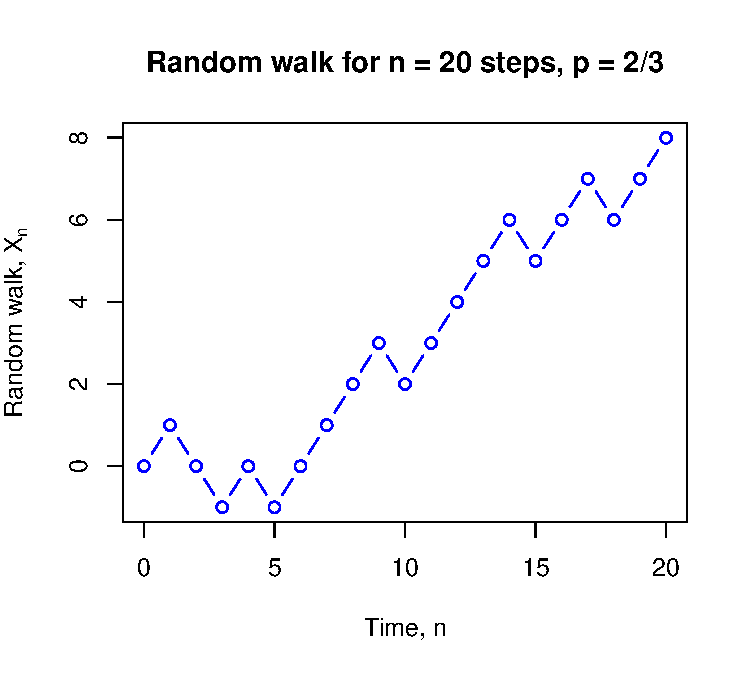
\includegraphics[width=0.5\linewidth]{math2750_files/figure-latex/rw-pics-1} 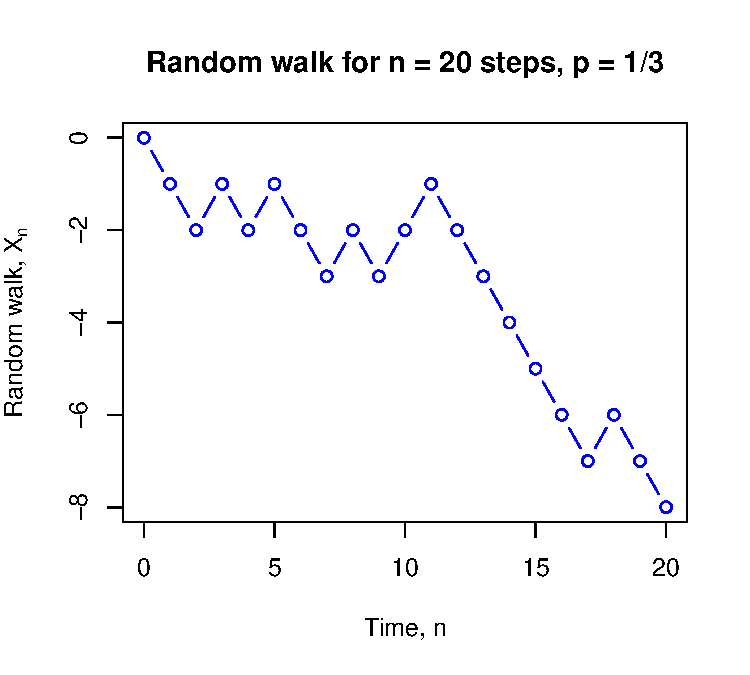
\includegraphics[width=0.5\linewidth]{math2750_files/figure-latex/rw-pics-2} \caption{Two simulations of random walks.}\label{fig:rw-pics}
\end{figure}

We can write this as a stochastic process \((X_n)\) with discrete time \(n = \{0,1,2,\dots\} = \mathbb Z_+\) and discrete state space \(\mathcal S = \mathbb Z\), where \(X_0 = 0\) and, for \(n \geq 0\), we have
\[ X_{n+1} = \begin{cases} X_n + 1 & \text{with probability $p$,} \\
                             X_n - 1 & \text{with probability $q$.} \end{cases} \]

It's clear from this definition that \(X_{n+1}\) (the future) depends on \(X_n\) (the present), but, given \(X_n\), does not depend on \(X_{n-1}, \dots, X_1, X_0\) (the past). Thus the Markov property holds, and the simple random walk is a \textbf{discrete time Markov process} or \textbf{Markov chain}.

\begin{example}
\protect\hypertarget{exm:rw1}{}\label{exm:rw1}

\emph{What is the probability that after two steps a simple random walk has reached \(X_2 = 2\)?}

To achieve this, the walk must go upwards in both time steps, so \(\mathbb P(X_2 = 2) = pp = p^2\).

\end{example}

\begin{example}
\protect\hypertarget{exm:rw2}{}\label{exm:rw2}

\emph{What is the probability that after three steps a simple random walk has reached \(X_3 = -1\)?}

There are three ways to reach \(-1\) after three steps: up--down--down, down--up--down, or down--down--up. So
\[ \mathbb P(X_3 = -1) = pqq+qpq+qqp = 3pq^2 . \]

\end{example}

\hypertarget{general-random-walks}{%
\subsection{General random walks}\label{general-random-walks}}

An alternative way to write the simple random walk is to put
\begin{equation}
    X_n = X_0 + \sum_{i=1}^n Z_i ,  \label{eq:rw}
  \end{equation}
where the starting point is \(X_0 = 0\) and the \textbf{increments} \(Z_1, Z_2, \dots\) are independent and identically distributed (IID) random variables with distribution given by \(\mathbb P(Z_i = 1) = p\) and \(\mathbb P(Z_i = -1) = q\). You can check that \eqref{eq:rw} means that \(X_{n+1} = X_n + Z_{n+1}\), and that this property defines the simple random walk.

Any stochastic process with the form \eqref{eq:rw} for some \(X_0\) and some distribution for the IID \(Z_i\)s is called a \textbf{random walk} (without the word ``simple'').

Random walks often have state space \(\mathcal S = \mathbb Z\), like the simple random walk, but they could be defined on other state spaces. We could look at higher dimensional simple random walks: in \(\mathbb Z^2\), for example, we could step up, down, left or right each with probability \(\frac14\). We could even have a continuous state space like \(\mathbb R\), if, for example, the \(Z_i\)s had a normal distribution.

We can use this structure to calculate the expectation or variance of any random walk (including the simple random walk).

Let's start with the expectation. For a random walk \((X_n)\) we have
\[ \mathbb E X_n = \mathbb E \left(X_0 + \sum_{i=1}^n Z_i\right) = \mathbb E X_0 + \sum_{i=1}^n \mathbb E Z_i = \mathbb EX_0 + n \mathbb E Z_1 , \]
where we've used the linearity of expectation, and that the \(Z_i\)s are identically distributed.

In the case of the simple random walk, we have \(\mathbb E X_0 = 0\), since we start from \(0\) with certainty, and
\[ \mathbb E Z_1 = \sum_{z \in \mathbb Z} z \mathbb P(Z_1 = z) = 1\times p + (-1)\times q = p-q .\]
Hence, for the simple random walk, \(\mathbb EX_n = n(p-q)\).

If \(p > \frac12\), then \(p > q\), so \(\mathbb E X_n\) grows ever bigger over time, while if \(p < \frac12\), then \(\mathbb E X_n\) grows ever smaller (that is, negative with larger absolute value) over time. If \(p = \frac12 = q\), which is the case of the simple symmetric random walk, then then the expectation \(\mathbb E X_n = 0\) is zero for all time.

Now the variance of a random walk. We have
\[ \operatorname{Var}(X_n) = \operatorname{Var}\left(X_0 + \sum_{i=1}^n Z_i\right) = \operatorname{Var}X_0 + \sum_{i=1}^n \operatorname{Var}Z_i = \operatorname{Var}X_0 + n \operatorname{Var}Z_1 , \]
where it was crucial that \(X_0\) and all the \(Z_i\)s were independent (so we had no covariance terms).

For the simple random walk we have \(\operatorname{Var}X_0 = 0\), since we always start from \(0\) with certainty. To calculate the variance of the increments, we write
\begin{align*}
  \operatorname{Var}(Z_1) &= \mathbb E (Z_1 - \mathbb EZ_1)^2 \\
            &= p\big(1 - (p-q)\big)^2 + q \big( {-1} - (p-q)\big)^2\\
            &= p(2q)^2 + q(-2p)^2\\
            &= 4pq^2 + 4p^2q \\
            &= 4pq(p+q) \\
            &= 4pq .
  \end{align*}
Here we've used that \(1-p = q\), \(1-q=p\), and \(p+q = 1\); you should take a few moments to check you've followed the algebra here. Hence the variance of the simple random walk is \(4pqn\). We see that (unless \(p\) is \(0\) or \(1\)) the variance grows over time, so it becomes harder and harder to predict where the random walk will be.

The variance of the simple symmetric random walk is \(4 \frac12 \frac12 n = n\).

For large \(n\), we can use a normal approximation for a random walk. Suppose the increments process \((Z_n)\) has mean \(\mu\) and variance \(\sigma^2\), and that the walk starts from \(X_0 = 0\). Then we have \(\mathbb E X_n = \mu n\) and \(\operatorname{Var}(X_n) = \sigma^2 n\), so for large \(n\) we can use the normal approximation \(X_n \approx \mathrm{N}(\mu n, \sigma^2 n)\). (Remember, of course, that the \(X_n\) are not independent.) To be more formal, the central limit theorem tells us that, as \(n \to \infty\), we have
\[ \frac{X_n - n\mu}{\sigma \sqrt{n}} \to \mathrm{N}(0,1) . \]

\hypertarget{exact-distribution}{%
\subsection{Exact distribution of the simple random walk}\label{exact-distribution}}

In the case of the simple random walk, we can in fact give the exact distribution by writing down an exact formula for \(\mathbb P(X_n = i)\) for any time \(n\) and any state \(i\).

Recall that, at each of the first \(n\) times, we independently take an upward step with probability \(p\), and otherwise take a downward step. So if we let \(Y_n\) be the number of upward steps over the first \(n\) time periods, we see that \(Y_n\) has a binomial distribution \(Y_n \sim \text{Bin}(n,p)\).

Recall that the binomial distribution has probability
\[  \mathbb P(Y_n = k)  = \binom nk p^k (1-p)^{n-k} = \binom nk p^k q^{n-k} , \]
for \(k = 0,1,\dots, n\), where \(\binom{n}{k}\) is the binomial coefficient ``\(n\) choose \(k\)''.

If \(Y_n = k\), that means we've taken \(k\) upward steps and \(n-k\) downward steps, leaving us at position \(k - (n-k) = 2k - n\). Thus we have that
\begin{equation}
  \mathbb P(X_n = 2k - n) = \mathbb P(Y_n = k) = \binom nk p^k q^{n-k} .  \label{eq:bin}
  \end{equation}

Note that after an odd number of time steps \(n\) we're always at an odd-numbered state, since \(2k - \text{odd} = \text{odd}\), while after an even number of time steps \(n\) we're always at an even-numbered state, since \(2k - \text{even} = \text{even}\).

Writing \(i = 2k - n\) gives \(k = (n+i)/2\) and \(n-k = (n-i)/2\). So we can rearrange \eqref{eq:bin} to see that the distribution for the simple random walk is
\[ \mathbb P(X_n = i) =  \binom{n}{(n+i)/2} p^{(n+i)/2} q^{(n-i)/2} , \]
when \(n\) and \(i\) have the same parity with \(-n \leq i \leq n\), and is \(0\) otherwise.

In the special case of the simple symmetric random walk, we have
\[ \mathbb P(X_n = i) = \binom{n}{(n+i)/2} \left(\frac12\right)^{(n+i)/2} \left(\frac12\right)^{(n-i)/2} = \binom{n}{(n+i)/2} 2^{-n} . \]

\textbf{In the next section}, we look at a gambling problem based on the simple random walk.

\hypertarget{P01}{%
\section*{Problem Sheet 1}\label{P01}}
\addcontentsline{toc}{section}{Problem Sheet 1}

You should attempt all these questions and write up your solutions in advance of your workshop in week 2 (Monday 1 or Tuesday 2 February) where the answers will be discussed.

\textbf{1.} When designing a model for a quantity that changes over time, one has many decisions to make:

\begin{itemize}
\tightlist
\item
  Discrete or continuous state space?
\item
  Discrete or continuous index set for time?
\item
  Deterministic or stochastic model?
\item
  If a stochastic model is chosen, is it reasonable to assume that the Markov property holds?
\end{itemize}

What would you decide for the following scenarios:

\textbf{(a)} The percentage of US voters with a positive opinion of Donald Trump in the Gallup weekly tracking poll.

\textbf{(b)} The number of points won by a football league club throughout the season.

\textbf{(c)} The temperature of a bowl of water placed in an oven.

\textbf{(d)} The number of people inside the Chemistry building.

\begin{myanswers}

\emph{Suggestions.} This question is meant to inspire discussion, so there are not necessarily right and wrong answers. If I were designing the models, however, my choices might be these:

\textbf{(a)} Discrete space if percentages are given to nearest 1\%, otherwise continuous; discrete time (weekly); stochastic; the Markov property might be appropriate, perhaps using some sort of random walk.

\textbf{(b)} Discrete space (number of points); discrete time (update after each game); stochastic; the Markov property might be appropriate, depending on if you think teams can have non-Markovian ``winning streaks'' (or losing streaks) that don't reflect underlying performance.

\textbf{(c)} Continuous space (temperature); continuous time; if the oven is reliable and the experiment carried out carefully, a deterministic model might be sufficient.

\textbf{(d)} Discrete space (number of people); continuous time; stochastic; Markov property might not be appropriate due to `bursts' of people leaving during fire drills or lectures finishing early.

\end{myanswers}

\textbf{2.} A fair six-sided dice is rolled twice, resulting in the
values \(X_1, X_2 \in \{1, 2, \ldots, 6\}\). Let \(Y = X_1 + X_2\) be the total score.
Calculate:

\textbf{(a)} the probability \(\mathbb P(Y = 10)\);

\begin{myanswers}

\emph{Solution.} The following table illustrates the possible outcomes \(Y\) of the experiment. Each cell of the table is an equally probable outcome.

\begin{center}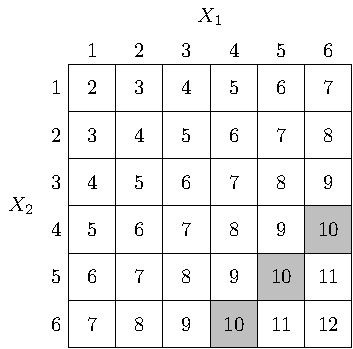
\includegraphics{math2750_files/figure-latex/dice-1} \end{center}

There are 3 possible ways to get \(Y=10\) (the grey cells in the table) out of the \(36\) possible outcomes, so we have \(\mathbb P(Y = 10) = 3/36 = 1/12\).

\end{myanswers}

\textbf{(b)} the conditional probability \(\mathbb P(Y=10 \mid X_1=x)\) for \(x=1, 2, \ldots, 6\);

\begin{myanswers}

\emph{Solution.} Conditioning on \(X_1 = x\) means restricting our attention only to column \(x\) of the table. Each column has \(6\) equally probably cells. For \(x=1,2,3\), none of the entries equal \(10\), so \(\mathbb P(Y=10 \mid X_1=x) = 0/6 = 0\). For each of \(x=4,5,6\), one of the entries equals \(10\), so \(\mathbb P(Y=10 \mid X_1=x) = 1/6\).

\end{myanswers}

\textbf{(c)} the conditional probability \(\mathbb P(X_1=x \mid Y=10)\) for \(x=1, 2, \ldots, 6\).

\begin{myanswers}

\emph{Solution.} Conditioning on \(Y =10\) means restricting our attention only to the \(3\) shaded cells, which are each equally likely. For \(x=1,2,3\), none of the shaded cells are in column \(x\), so \(\mathbb P(X_1=x \mid Y=10) = 0/3 = 0\). For each of \(x=4,5,6\), one of the shaded cells is in column \(x\), so \(\mathbb P(X_1=x \mid Y=10) = 1/3\).

\end{myanswers}

\textbf{3.} Let \((X_n)\) be a simple random walk starting from \(X_0 = 0\) and that at each step goes up one with probability \(p\) or down one with probability \(q = 1-p\). What are:

\textbf{(a)} \(\mathbb P(X_5 = 3)\),

\begin{myanswers}

\emph{Solution.} To get \(X_5 = 3\), we must take \(4\) steps up and \(1\) step down. The down step can be at any of the \(5\) time steps. Therefore we have \(\mathbb P(X_5 = 3) = 5p^4q\).

\end{myanswers}

\textbf{(b)} \(\mathbb P(X_5 = 3 \mid X_2 = 2)\),

\begin{myanswers}

\emph{Solution.} Once we're at \(X_2 = 2\), we must take \(2\) steps up and \(1\) step down over the next \(3\) time steps. So \(\mathbb P(X_5 = 3 \mid X_2 = 2) = 3p^2q\).

\end{myanswers}

\textbf{(c)} \(\mathbb P(X_n = n-2)\),

\begin{myanswers}

\emph{Solution.} This requires \(n-1\) steps up and \(1\) step down, and the down step can be at any of the \(n\) time steps. So \(\mathbb P(X_n = n-2) = np^{n-1}q\).

\end{myanswers}

\textbf{(d)} \(\mathbb E X_4\),

\begin{myanswers}

\emph{Solution.} The increments \(Z_n = X_n - X_{n-1}\) have expectation \(1p + (-1)q = p - q\), so \(\mathbb E X_4 = 4(p-q)\).

\end{myanswers}

\textbf{(e)} \(\mathbb E(X_6 \mid X_4 = 2)\),

\begin{myanswers}

\emph{Solution.} We are already at 2, then another two increments will take us up \(2(p-q)\) on average. Therefore \(\mathbb E(X_6 \mid X_4 = 2) = 2 + 2(p-q)\).

\end{myanswers}

\textbf{4.} The price \(X_n\) of a stock at the close of day \(n\) is modelled as a Gaussian random walk, where the increments \((Z_n)\) have a normal distribution \(Z_n \sim \text{N}(\mu, \sigma^2)\). The model assumes a drift of \(\mu = 0.7\) and a volatility of \(\sigma = 2.2\). The initial price is \(X_0 = 42.3\).

\textbf{(a)} Calculate the mean and variance of the price of the stock at the close of day \(5\).

\begin{myanswers}

\emph{Solution.} The mean and variance are
\begin{gather*}
  \mathbb EX_5 = \mathbb E X_0 + n \mathbb E Z_1 = 42.3 + 5 \cdot 0.7 = 45.8 , \\
  \operatorname{Var}X_5 = \operatorname{Var}X_0 + n \operatorname{Var}Z_1 = 0 + 5 (2.2)^2 = 24.2 .
  \end{gather*}

\end{myanswers}

\textbf{(b)} Give a 95\% prediction interval for the price at the close of day 5. (You might find it useful to recall that, if \(W \sim \text{N}(0,1)\) is a standard normal random variable, then \(\mathbb P(W \leq 1.96) = 0.975\).)

\begin{myanswers}

\emph{Solution.} Note that \(X_5\) itself is normally distributed, so \(X_5 \sim \text{N}(45.8,24.2)\). The 95\% prediction interval for a normal distribution \(\text{N}(\mu, \sigma^2)\) is \((\mu - 1.96\sigma, \mu + 1.96\sigma)\), so the prediction interval for \(X_5\) is
\[ \big(45.8 - 1.96\sqrt{24.2},  45.8 + 1.96\sqrt{24.2}\big) = (36.16, 55.44) . \]

\end{myanswers}

\textbf{(c)} After day 4, the prices at the end of each of the first four days have been recorded as \(X_1 = 44.4, X_2 = 44.0, X_3 = 47.1, X_4 = 47.8\). Update your prediction interval for the price at the close of day 5, and comment on how it differs from the earlier prediction interval.

\begin{myanswers}

\emph{Solution.} By the Markov property, \(X_5\) depends on \(X_4\), but given \(X_4\) does not depend on the other values, which we can therefore ignore. Since \(X_5 = X_4 + Z_5\), we have
\begin{gather*}
  \mathbb E(X_5 \mid X_4) = X_4 + \mathbb E Z_5 = 47.8 + 0.7 = 48.5 \\
  \operatorname{Var}(X_5 \mid X_4) = 0 + \operatorname{Var}Z_5 = 0 + (2.2)^2 = 4.84.
  \end{gather*}
The desired prediction interval is
\[ \big(48.5 - 1.96\sqrt{4.84},  48.5+ 1.96\sqrt{4.84}\big) = (44.19, 52.81) . \]
Compared to before, the centre of the prediction interval is slightly higher, because the stock has outperformed expectations so far, and the interval is much narrower, because as we get closer to day 5 we become less uncertain.

\end{myanswers}

\textbf{5.} A gambler decides to model her total winnings as a simple random walk starting from \(X_0 = 0\) that at each time goes up one with probability \(p\) and down one with probability \(1-p\), but where \(p\) is unknown. The first \(10\) recordings, \(X_1\) to \(X_{10}\), are
\[ (1, 2, 1, 2, 3, 4, 5, 6, 5, 6) . \]

\textbf{(a)} What would you guess for the value of \(p\), given this data?

\begin{myanswers}

\emph{Solution.} In \(10\) time steps, the process went up \(k = 8\) times and down \(n - k = 2\) times. So it seems reasonable to guess that \(p\) has the value \(\hat p = 8/10 = 0.8\).

\end{myanswers}

\textbf{(b)} More generally, how would you estimate \(p\) from the data \(X_0 = 0, X_1 = x_1, X_2 = x_2, \dots, X_n = x_n\)?

\begin{myanswers}

\emph{Solution.} We will estimate \(\hat p = k/n\), where \(k\) is the number of upward steps. We saw in lectures that \(k = (n + x_n)/2\), so our estimate is
\[ \hat p = \frac{n + x_n}{2n} = \frac12\ + \frac{x_n}{2n} . \]

\end{myanswers}

\textbf{(c)} Show that your estimate is in fact the maximum likelihood estimate of \(p\).

\begin{myanswers}

\emph{Solution.} You could answer this question by using what you know about maximum likelihood estimation for the binomial distribution from MATH1712, but we'll reason from first principles here.

If we let \(k\) be the number of upward steps, then the likelihood is
\[ f(\mathbf x; p) = p^{k}(1-p)^{n-k} , \]
making the the log-likelihood
\[ \ell(\mathbf x; p) = \ln f(\mathbf x; p) = k \ln p + (n-k)\ln(1-p) .\]
We maximise this by differentiating and setting equal to \(0\). The derivative is
\[ \frac{\text{d}}{\text{d}p} \ell(\mathbf x; p) = \frac kp - \frac{n-k}{1-p} ,\]
so the maximum likelihood estimate \(\hat p\) satisfies
\[ 0 = \frac k{\hat p} - \frac{n-k}{1-\hat p} . \]
Solving this by clearing denominators we get
\[ 0 = (k - k\hat p) - (n\hat p - k\hat p) = k - n \hat p , \]
and rearranging gives \(\hat p = k/n\) as desired.

\end{myanswers}

\hypertarget{S03-gamblers-ruin}{%
\section{Gambler's ruin}\label{S03-gamblers-ruin}}

\begin{itemize}
\tightlist
\item
  The gambler's ruin Markov chain
\item
  Equations for probability of ruin and expected duration of the game by conditioning on the first step
\end{itemize}

\hypertarget{ruin-chain}{%
\subsection{Gambler's ruin Markov chain}\label{ruin-chain}}

Consider the following gambling problem. Alice is gambling against Bob. Alice starts with £\(a\) and Bob starts with £\(b\). It will be convenient to write \(m = a + b\) for the total amount of money, so Bob starts with £\((m-a)\). At each step of the game, both players bet £\(1\); Alice wins £\(1\) off Bob with probability \(p\), or Bob wins £\(1\) off Alice with probability \(q\). The game continues until one player is out of money (or is ``ruined'').

Let \(X_n\) denote how much money Alice has after \(n\) steps of the game. We can write this as a stochastic process with discrete time \(n \in \{0,1,2,\dots\} = \mathbb Z_+\) and discrete state space \(\mathcal S = \{0,1,\dots,m\}\). Then \(X_0 = a\), and, for \(n \geq 0\), we have
\[ X_{n+1} = \begin{cases} X_n + 1 & \text{with probability $p$ if $1\leq X_n \leq m-1$,} \\
                           X_n - 1 & \text{with probability $q$ if $1\leq X_n \leq m-1$,} \\
                           0       & \text{if $X_n = 0$,} \\
                           m       & \text{if $X_n = m$.} \end{cases} \]
So Alice's money goes up one with probability \(p\) or down one with probability \(q\), unless the game is already over with \(X_n = 0\) (Alice is ruined) or \(X_n = m\) (Alice has won all Bob's money, so Bob in ruined).

We see that the gambler's ruin process \((X_n)\) clearly satisfies the Markov property: the next step \(X_{n+1}\) depends on where we are now \(X_n\), but, given that, does not depend on how we got here.

The gambler's ruin process is exactly like a simple random walk started from \(X_0 = a\) except that we have \textbf{absorbing barriers} and \(0\) and \(m\), where the random walk stops because one of the players has ruined. (One could also consider random walks with \textbf{reflecting barriers}, that bounce the random walk back into the state space, or \textbf{mixed barriers} that are absorbing or reflecting at random.)

\hypertarget{ruin-probability}{%
\subsection{Probability of ruin}\label{ruin-probability}}

The gambling game continues until either Alice is ruined (\(X_n = 0\)) or Bob is ruined (\(X_n = m\)). A natural question to ask is: What is the probability that the game ends in Alice's ruin?

Let us write \(r_i\) for the probability Alice ends up ruined if she currently has £\(i\). Then the probability of ruin for the whole game is \(r_a\), since Alice initially starts with £\(a\). The probability Bob will end up ruined is \(1 - r_a\), since one of the players must lose.

What can we say about \(r_i\)? Clearly we have \(r_0 = 1\) and \(r_m = 0\), since this means Alice (\(i=0\)) or Bob (\(i=m\)) is already out of money and is ruined. What about for \(1 \leq i \leq m-1\)?

The key is to \emph{condition on the first step}. That is, we can write
\begin{align*}
\mathbb P(\text{ruin}) &= \mathbb P(\text{win first round}) \, \mathbb P(\text{ruin} \mid \text{win first round}) \\
&\qquad{}+ \mathbb P(\text{lose first round}) \, \mathbb P(\text{ruin} \mid \text{lose first round}) \\
&= p\,\mathbb P(\text{ruin} \mid \text{win first round}) + q \,\mathbb P(\text{ruin} \mid \text{lose first round}) .
\end{align*}
Here we have conditioned on whether Alice wins or loses the first round. More formally, we have used the \emph{law of total probability}, which says that if the disjoint events \(B_1, \dots, B_k\) cover the whole sample space, then
\[ \mathbb P(A) = \sum_{i=1}^k \mathbb P(A \cap B_i) = \sum_{i=1}^k \mathbb P(B_i) \, \mathbb P(A \mid B_i) . \]
Here, \(\{\text{Alice wins the first round}\}\) and \(\{\text{Alice loses the first round}\}\) are indeed disjoint events that cover the whole sample space. This idea of ``conditioning on the first step'' will be the most crucial tool throughout this whole module.

If Alice wins the first round from having £\(i\), she now has £\((i+1)\). Her probability of ruin is now \(r_{i+1}\), because, by the Markov property, it's as if the game were starting again with Alice having £\((i+1)\) to start with. The Markov property tells us that it doesn't matter \emph{how} Alice got to having £\((i+1)\), it only matters how much she has now. Similarly, if Alice loses the first round, she now has £\((i-1)\), and the ruin probability is \(r_{i-1}\). Hence we have
\[ r_i = pr_{i+1} + qr_{i-1}. \]

Rearranging, and including the ``boundary conditions'', we see that the equation we want to solve is
\[ pr_{i+1} - r_i + qr_{i-1} = 0 \qquad \text{subject to} \qquad r_0 = 1,\ r_m = 0. \]
This is a \textbf{linear difference equation} -- and, because the left-hand side is \(0\), we call it a \textbf{homogeneous} linear difference equation.

We will see how to solve this equation in the next lecture. We will see that, if we set \(\rho = q/p\), then the ruin probability is given by
\[ r_a = \begin{cases} \displaystyle\frac{\rho^a - \rho^m}{1 - \rho^m} & \text{if $\rho \neq 1$,} \\[0.35cm]
           1 - \displaystyle\frac{a}{m} & \text{if $\rho = 1$.} \end{cases} \]
Note that \(\rho = 1\) is the same as the symmetric condition \(p = q = \frac12\).

Imagine Alice is not playing against her opponent Bob, but rather is up against a large casino. In this case, the casino's capital £\((m-a)\) is typically much bigger than Alice's £\(a\). We can model this by keeping \(a\) fixed taking a limit \(m \to \infty\). Typically, the casino has ``an edge'', meaning they have a better than \(50:50\) chance of winning; this means that \(q > p\), so \(\rho > 1\). In this case, we see that the ruin probability is
\[ \lim_{m \to \infty} r_a = \lim_{m \to \infty} \frac{\rho^a - \rho^m}{1 - \rho^m} = \lim_{m \to \infty} \frac{\rho^a/\rho^m - 1}{1/\rho^m - 1} = \frac{0-1}{0-1} = 1, \]
so Alice will be ruined with certainty.

Even with a generous casino that offered an exactly fair game with \(p = q = \frac12\), so \(\rho = 1\), we would have
\[ \lim_{m \to \infty} r_a = \lim_{m \to \infty}\left( 1 - \frac{a}{m} \right) = 1-0 = 1 , \]
so, even with this fair game, Alice would still be ruined with certainty.

The official advice of the University of Leeds module MATH2750 is that you shouldn't gamble against a casino and expect to win.

\hypertarget{expected-duration}{%
\subsection{Expected duration of the game}\label{expected-duration}}

We could also ask for how long we expect the game to last.

We approach this like before. Let \(d_i\) be the expected duration of the game when Alice has £\(i\). Our boundary conditions are \(d_0 = d_m = 0\), because \(X_n = 0\) or \(X_n = m\) means that the game is over with Alice or Bob ruined. Again, we proceed by conditioning on the first step, so
\begin{align*}
\mathbb E(\text{duration}) &= \mathbb P(\text{win first round}) \, \mathbb E(\text{duration} \mid \text{win first round}) \\
&\qquad{}+ \mathbb P(\text{lose first round}) \, \mathbb E(\text{duration} \mid \text{lose first round}) \\
&= p\,\mathbb E(\text{duration} \mid \text{win first round}) + q \,\mathbb E(\text{duration} \mid \text{lose first round}) .
\end{align*}
More formally, we've used another version of the law of total probability,
\[ \mathbb E(X) = \sum_{i=1}^k \mathbb P(B_i) \, \mathbb E(X \mid B_i) , \]
or, alternatively, the \emph{tower law} for expectations
\[ \mathbb E(X) = \mathbb E_Y \mathbb E (X \mid Y) = \sum_{y} \mathbb P(Y= y)\, E(X \mid Y = y), \]
where, in our case, \(Y\) was the outcome of the first round.

Now, the expected duration given we win the first round is \(1 + d_{i+1}\). This is because the round itself takes \(1\) time step, and then, by the Markov property, it's as if we are starting again from \(i+1\). Similarly, the expected duration given we lose the first round is \(1 + d_{i-1}\). Thus we have
\[ d_i = p(1 + d_{i+1}) + q (1 + d_{i-1}) = 1 + pd_{i+1} + qd_{i-1} . \]
Don't forget the 1 that counts the current round!

Rearranging, and including the boundary conditions, we have another linear difference equation:
\[ pd_{i+1} - d_i + qd_{i-1} = -1 \qquad \text{subject to} \qquad d_0 = 0,\ d_m = 0. \]
Because the right-hand side, \(-1\), is nonzero, we call this an \textbf{inhomogeneous} linear difference equation.

Again, we'll see how to solve this in the next lecture, and will find that the solution is given by
\[ d_a = \begin{cases} {\displaystyle \frac{1}{q-p} \left(a - m\frac{1-\rho^a}{1- \rho^m} \right)} & \text{if $\rho \neq 1$,} \\
\displaystyle a(m-a) & \text{if $\rho = 1$.} \end{cases} \]

Thinking again of playing against the casino, with \(q > p\), \(\rho > 1\), and \(m \to \infty\), we see that the expected duration is
\[ \lim_{m\to\infty} d_a = \lim_{m\to\infty} \frac{1}{q-p} \left(a - m\frac{1-\rho^a}{1 - \rho^m} \right)  = \frac{1}{q-p} \left(a - 0 \right) = \frac{a}{q-p} , \]
since \(\rho^m\) grows much quicker than \(m\). So Alice ruins with certainty, and it will take time \(a/(q-p)\), on average.

In the case of the generous casino, though, with \(q = p\), so \(\rho = 1\), we have
\[ \lim_{m\to\infty} d_a =  \lim_{m\to\infty} a(m-a) = \infty .  \]
So here, Alice will ruin with certainty, but it may take a very long time until the ruin occurs, since the expected duration is infinite.

\textbf{In the next section}, we see how to solve linear difference equations, in order to find the ruin probability and expected duration of the gambler's ruin.

\hypertarget{S04-ldes}{%
\section{Linear difference equations}\label{S04-ldes}}

\begin{itemize}
\tightlist
\item
  How to solve homogeneous and inhomogeneous linear difference equations
\item
  Solving for probability of ruin and expected duration of the gambler's ruin
\end{itemize}

\textbf{Linear difference equations} are equations that look like
\begin{equation}
a_k x_{n+k} + a_{k-1} x_{n+k-1} + \cdots + a_1 x_{n+1} + a_0 x_n = f(n) \label{eq:lde} 
\end{equation}
for \(n = 0,1,\dots\), where the \(a_i\) are given constants, \(f(n)\) is a given function, and we want to solve for the sequence \((x_n)\). The equation normally comes with some extra conditions, such as the value of the first few \(x_n\)s.

When the right-hand side of \eqref{eq:lde} is zero, so \(f(n) = 0\), we say the equation is \textbf{homogeneous}; if the right-hand side is nonzero, it is \textbf{inhomogeneous}. The number \(k\), where there are \(k+1\) terms on the left-hand side, is called the \textbf{degree} of the equation; we are mostly interested in second-degree linear difference equations, which have three terms on the left-hand side.

\hypertarget{hom-ldes}{%
\subsection{Homogeneous linear difference equations}\label{hom-ldes}}

We start with the homogeneous case, which is simpler.

Consider a homogeneous linear difference equation. We shall use the second-degree example
\[ x_{n+2} - 5x_{n+1} + 6x_{n} = 0 \qquad \text{subject to } x_0 = 4, x_1 = 9 .  \]
Here, the conditions on \(x_0\) and \(x_1\) are \textbf{initial conditions}, because they tell us how the sequence \((x_n)\) starts.

For the moment, we shall put the initial conditions to the side and just worry about the equation
\[ x_{n+2} - 5x_{n+1} + 6x_{n} = 0 . \]
We start by guessing there might be a solution of the form \(x_n = \lambda^n\) for some constant \(\lambda\). We can find out if there is such a solution by substituting in \(x_n = \lambda^n\), and seeing if there's a \(\lambda\) that solves the equation. For our example, we get
\[ \lambda^{n+2} - 5 \lambda^{n+1} + 6\lambda^n = 0 . \]
After cancelling off a common factor of \(\lambda^n\), we get
\[ \lambda^2 - 5 \lambda + 6 = 0 . \]
This is called the \textbf{characteristic equation}. For a general homogeneous linear difference equation \eqref{eq:lde}, the characteristic equation is
\begin{equation}
  a_k \lambda^{k} + a_{k-1} \lambda^{k-1} + \cdots + a_1 \lambda + a_0 = 0 .  \label{eq:cheq} 
\end{equation}
When writing out answers to questions, you can jump straight to the characteristic equation.

We can now solve the characteristic equation for \(\lambda\). In our example, we can factor the left-hand side to get \((\lambda - 3)(\lambda - 2) = 0\), which has solutions \(\lambda = 2\) and \(\lambda = 3\). Thus \(x_n = 2^n\) and \(x_n = 3^n\) both solve our equation. In fact, since the right-hand side of the equation is \(0\), any linear combination of these two solutions is a solution also, thus we get the \textbf{general solution}
\[ x_n = A 2^n + B 3^n , \]
which is a solution for any values of the constants \(A\) and \(B\).

For a general characteristic equation with distinct roots \(\lambda_1, \lambda_2, \dots, \lambda_k\), the general solution is
\[ x_n = C_1 \lambda_1^n + C_2 \lambda_2^n + \cdots + C_k \lambda_k^n . \]
If we have a repeated root -- say, \(\lambda_1 = \lambda_2 = \cdots = \lambda_r\) is repeated \(r\) times -- than you can check that a solution is given by
\[ x_n = (D_0 + D_1 n + \cdots + D_{r-1} n^{r-1}) \lambda_1^n , \]
which should take its place in the general solution.

Once we have the general solution, we can use the extra conditions to find the values of the constants. In our example, we can use the initial conditions to find out the values of \(A\) and \(B\). We see that
\begin{gather*}
x_0 = A2^0 + B3^0 = A + B = 4 , \\
x_1 = A2^1 + B3^1 = 2A + 3B = 9 .
\end{gather*}
We can now solve this pair of simultaneous equations to solve for \(A\) and \(B\). By subtracting twice the first equation from the second we get \(B = 1\), and substituting this into the first equation we get \(A = 3\). Thus the solution is
\[ x_n = 3\cdot 2^n + 3^n . \]

In conclusion, the process here was:

\begin{enumerate}
\def\labelenumi{\arabic{enumi}.}
\tightlist
\item
  Find the general solution by writing down and solving the characteristic equation.
\item
  Use the extra conditions to find the values of the constants in the general solution.
\end{enumerate}

If you think you've got the hang of this, you should press on to \protect\hyperlink{S04-ruin-probability}{the next subsection}. But if you're still a bit unsure, here are two extra optional examples. (These also give an idea of how I would expect you to set out your answers to similar problems.)

\begin{example}
\protect\hypertarget{exm:lde1}{}\label{exm:lde1}

\emph{Solve the homogeneous linear difference equation}
\[ x_{n+2} - x_{n+1} - 6x_n = 0 \qquad \text{subject to} \quad x_0 = 3,\quad x_1 = 4 . \]

\emph{Step 1.} The characteristic equation is
\[ \lambda^2 - \lambda - 6 = 0 . \]
We can solve this by factorising it as \((\lambda - 3) (\lambda + 2) = 0\),
to find the solutions \(\lambda_1 = -2\) and \(\lambda_2 = 3\). Thus the general solution is
\[ x_n = A(-2)^n + B3^n . \]

\emph{Step 2.} Substituting the initial conditions into the general solution, we have
\begin{align*}
x_0 &= A(-2)^0 + B3^0 = A + B = 3 \\
x_1 &= A(-2)^1 + B3^1 = -2A + 3B = 4 .
\end{align*}
We can add twice the first equation from the second to get \(5B = 10\), so \(B=2\). We can substitute this into the first equation to get \(A = 1\).

The solution is therefore
\[ x_n = 1\cdot(-2)^n + 2 \cdot 3^n = (-2)^n + 2 \cdot 3^n . \]

\end{example}

\begin{example}
\protect\hypertarget{exm:lde2}{}\label{exm:lde2}

\emph{Solve the homogeneous linear difference equation}
\[ x_{n+2} + 4x_{n+1} +4x_n = 0 \qquad \text{subject to} \quad x_0 = 2,\quad x_1 = -6 . \]

\emph{Step 1.} The characteristic equation is
\[ \lambda^2 + 4\lambda + 4 = 0 . \]
We can solve this by factorising it as \((\lambda + 2)^2 = 0\), to find a repeated root \(\lambda_1 = \lambda_2 = -2\). Thus the general solution is
\[ x_n = (A + Bn) (-2)^n . \]

\emph{Step 2.} Substituting the initial conditions into the general solution, we have
\begin{align*}
x_0 &= (A + B0)(-2)^0 = A = 2 \\
x_1 &= (A + B1)(-2)^1 = -2A - 2B = -6 .
\end{align*}
The first immediately gives \(A = 2\), and substituting this into the second equation gives \(B = 1\).

The solution is therefore
\[ x_n = (2 + n)(-2)^n . \]

\end{example}

\hypertarget{ruin-probability-solve}{%
\subsection{Probability of ruin for the gambler's ruin}\label{ruin-probability-solve}}

In the last lecture we saw that probability of ruin for the gambler's ruin process is the solution to
\[ pr_{i+1} - r_i + qr_{i-1} = 0 \qquad \text{subject to} \qquad r_0 = 1,\ r_m = 0 , \]
where the extra conditions here are \textbf{boundary conditions}, because they tell us what happens at the boundaries of the state space.

The characteristic equation is
\[ p\lambda^2 - \lambda + q = 0 .\]
We can solve the characteristic equation by factorising it as \((p \lambda - q)(\lambda - 1) = 0\). (It might take a moment to check this really is a factorisation of the characteristic equation. Hint: we've used that \(p+q=1\).) So the characteristic equation has roots \(\lambda = q/p\), which we called \(\rho\) last time, and \(\lambda = 1\). Now, if \(\rho = 1\) (so \(p = q = \frac12\)) we have a repeated root, while if \(\rho \neq 1\) we have distinct roots, so we'll need to deal with the two cases separately.

First, the case \(\rho \neq 1\). Since the two roots are distinct, we have the general solution
\[ r_i = A\rho^i + B1^i = A\rho^i + B . \]

We can now use the boundary conditions to find \(A\) and \(B\). We have
\begin{gather*} r_0 = A \rho^0 + B = A+B = 1, \\
                r_m = A \rho^m + B = 0 . \end{gather*}
From the first we get \(B = 1-A\), which we substitute into the second to get
\[ A\rho^m + 1 - A = 0 \quad \Rightarrow \quad A = \frac{1}{1-\rho^m} , \]
and hence
\[ B = 1 - A = 1 - \frac{1}{1-\rho^m} = - \frac{\rho^m}{1 - \rho^m} . \]
Thus the solution is
\[ r_i = \frac{1}{1-\rho^m} \rho^i -  \frac{\rho^m}{1 - \rho^m} = \frac{\rho^i - \rho^m}{1 - \rho^m}  , \]
as we claimed last time.

Second, the case \(\rho = 1\). Now we have a repeated root \(\lambda = 1\), so the general solution is
\[ r_i = (A + Bi) 1^i = A+Bi . \]

Again, we use the boundary conditions, to get
\begin{gather*} r_0 = A + B\cdot 0 = A = 1, \\
r_m = A + Bm = 0 , \end{gather*}
and we immediately see that \(A = 1\) and \(B = -1/m\). Thus the solution is
\[ r_i = 1 - \frac{1}{m}i = 1 - \frac{i}{m} , \]
as claimed last time.

\hypertarget{inhom-ldes}{%
\subsection{Inhomogeneous linear difference equations}\label{inhom-ldes}}

Solving inhomogeneous linear difference equations requires three steps:

\begin{enumerate}
\def\labelenumi{\arabic{enumi}.}
\tightlist
\item
  Find the general solution to the \emph{homogeneous} equation by writing down and solving the characteristic equation.
\item
  Find any solution (a ``particular solution'') to the inhomogeneous equation. The general solution to the inhomogeneous equation is a particular solution plus the general solution to the homogeneous equation.
\item
  Use the extra conditions to find the values of the constants in the general solution.
\end{enumerate}

This idea works because adding a solution to the \emph{homogeneous} equation to the left-hand side adds zero to the right-hand side, so maintains a solution to the inhomogeneous equation.

Let's work through the example
\[ x_{n+2} - 5x_{n+1} + 6x_{n} = 2 \qquad \text{subject to } x_0 = 4, x_1 = 9 . \]

We already know from earlier that the general solution to the homogeneous equation \(x_{n+2} - 5x_{n+1} + 6x_{n} = 0\) (with a zero on the right-hand side) is
\[ x_n = A2^n + B3^n . \]

We now need to find a \textbf{particular solution} -- that is, any solution -- to our new inhomogeneous equation. A general hint here is to guess a solution with the same ``shape'' as the right-hand side. For example, if the right-hand side is a constant, try a constant for the particular solution. Here our right-hand side is the constant \(2\), so we should try a constant \(x_n = C\). Substituting this into the inhomogeneous equation gives us \(C - 5C + 6C = 2\), thus \(2C = 2\) and \(C = 1\), giving a particular solution \(x_n = 1\). The general solution to the inhomogeneous equation is therefore
\[ x_n = 1 + A2^n + B3^n , \]
the sum of the particular solution \(x_n = 1\) and the general solution to the homogeneous equation.

The right-hand side being a constant, so we guess a constant, is the main case we will deal with. Other cases you could come across include:

\begin{itemize}
\tightlist
\item
  If the right-hand side is a polynomial of degree \(d\), try a polynomial of degree \(d\).
\item
  If the right-hand side is \(\alpha^n\) for some \(\alpha\), try \(C\alpha^n\).
\item
  If the right-hand side is a constant, but a constant \(C\) doesn't work, try \(Cn\). If that still doesn't work, try \(Cn^2\), and so on. We discuss this case further in the next subsection.
\end{itemize}

Again, we use the initial conditions to get the constants \(A\) and \(B\). We have
\begin{gather*}
x_0 = 1 + A2^0 + B3^0 = 1+ A + B = 4 , \\
x_1 = 1 + A2^1 + B3^1 = 1+ 2A + 3B = 9 ,
\end{gather*}
and we can easily check this gives \(A = 1, B = 2\). Thus the solution is
\[ x_n = 1 + 1\cdot 2^n + 2 \cdot 3^n = 1 + 2^n + 2 \cdot 3^n . \]

Again, if you have the hang of this, \protect\hyperlink{duration-solve}{press on}, but we present an extra optional example if things are still unclear.

\begin{example}
\protect\hypertarget{exm:lde3}{}\label{exm:lde3}

\emph{Solve the inhomogeneous linear difference equation}
\[ 10 x_{n+2} - 7x_{n+1} + x_n = 8 \qquad \text{subject to} \quad x_0 = 0,\quad x_1 = \tfrac{13}{10} . \]

\emph{Step 1.} The characteristic equation is
\[ 10\lambda^2 - 7\lambda + 1 = 0 . \]
We can solve this by factorising it as
\[ (2\lambda - 1) (5\lambda - 1) = 0 , \]
to find the solutions \(\lambda_1 = \frac12\) and \(\lambda_2 = \frac15\). Thus the general solution of the homogeneous equation is
\[ x_n = A\left(\frac12\right)^n + B\left(\frac15\right)^n . \]

\emph{Step 2.} Since the right hand side of the inhomogeneous equation is a constant, we guess a constant particular solution with shape \(x_n = C\). Substituting in this guess, we get
\[ 10C - 7C + C = 4C = 8 \]
with solution \(C=2\). Thus a particular solution is \(x_n = 2\), and the general solution to the inhomogeneous equation is
\[ x_n = 2 + A\left(\frac12\right)^n + B\left(\frac15\right)^n . \]

\emph{Step 3.} Substituting the initial conditions into the general solution, we have
\begin{align*}
x_0 = 2 + A\left(\frac12\right)^0 + B\left(\frac15\right)^0 = 2 + A + B = 0 \quad &\Rightarrow \quad A + B = -2 \\
x_1 = 2 + A\left(\frac12\right)^1 + B\left(\frac15\right)^1 = 2 + A\frac12 + B\frac15 = \frac{13}{10} \quad &\Rightarrow \quad 5A + 2B = -7.
\end{align*}
We can subtract twice the first equation from the second to get \(3A = -3\), so \(A = -1\). We can substitute this into the second equation to get \(B = -1\).

The solution is therefore
\[ x_n = 2 - \left(\frac12\right)^n - \left(\frac15\right)^n . \]

\end{example}

\hypertarget{duration-solve}{%
\subsection{Expected duration for the gambler's ruin}\label{duration-solve}}

From last time, the expected duration of the gambler's ruin game solves
\[ pd_{i+1} - d_i + qd_{i-1} = -1 \qquad \text{subject to} \qquad d_0 = 0,\ d_m = 0. \]
As before, we divide cases based on whether or not \(\rho = 1\).

First, the case \(\rho \neq 1\). We already know that the general solution to the homogeneous equation is
\[ d_i =  A \rho^i + B . \]

Now we need a particular solution. It's tempting to guess a constant \(C\) for a particular solution, but we know that constants solve the homogeneous equation, since \(d_i = B\) is a solution -- so a constant will give right-hand side \(0\), not \(-1\). (You could try out \(x_i = C\); you should find that the equation for \(C\) doesn't have a solution.) The next best try is to go one degree up: let's guess \(x_i = Ci\) instead. This gives
\begin{align*}
  -1 &= pC(i+1) - Ci + qC(i-1)\\
     &= C(pi + p - i + qi - q) \\
     &= C\big((p+q-1)i + (p-q)\big) \\
     &= C(p-q) ,
  \end{align*}
since \(p + q - 1 = 1 - 1 = 0\). This \(C = -1/(p-q) = 1/(q-p)\). Finding a solution for \(C\) shows that our guess worked. The general solution to the inhomogeneous equation is
\[ d_i = \frac{i}{q-p} + A \rho^i + B .  \]

Then to find the constants, we have
\begin{gather*} d_0 = \frac{0}{q-p} + A \rho^0 + B = A+B = 0, \\
                  d_m = \frac{m}{q-p} + A \rho^m + B = 0 , \end{gather*}
which you can check gives
\[ A = -B = \frac{1}{q-p} \cdot \frac{m}{1 - \rho^m} . \]
Hence, the solution is
\[ d_i = \frac{i}{q-p} + \frac{1}{q-p} \cdot \frac{m}{1 - \rho^m} \rho^i - \frac{1}{q-p} \cdot \frac{m}{1 - \rho^m} =  \frac{1}{q-p} \left(i - m\frac{1-\rho^i}{1- \rho^m} \right) . \]

Second, the case \(\rho = 1\), so \(p = q = \frac12\). We already know that the general solution to the homogeneous equation is
\[ d_i =  A + Bi . \]

We need a particular solution. Since both constants \(x_i = A\) and linear \(x_i = Bi\) terms solve the homogeneous equation (or by checking that guessing \(x_i = C\) or \(x_i = Ci\) doesn't work), we'll have to go up another degree and try \(x_i = Ci^2\). This gives
\begin{align*}
    -1 &= \tfrac12 C(i+1)^2 - Ci^2 + \tfrac 12 C(i-1)^2 \\
       &= \tfrac12 C(i^2 + 2i + 1 - 2i^2 + i^2 - 2i + 1) \\
       &= \tfrac12 C\big((1-2+1)i^2 + (2-2)i + (1+1)\big) \\
       &=C ,
\end{align*}
so the general solution to the inhomogeneous equation is
\[ d_i = -i^2 + A + Bi .  \]

Then to find the constants, we have
\begin{gather*} d_0 = -0^2 + A + B\cdot0 = A = 0, \\
                  d_m = -m^2 + A + Bm = 0 , \end{gather*}
giving \(A = 0, B = m\). The solution is
\[ d_i = -i^2 + 0 + mi = i(m-i) .\]

\textbf{In the next section}, we move on to the general theory of discrete time Markov chains.

\hypertarget{P02}{%
\section*{Problem sheet 2}\label{P02}}
\addcontentsline{toc}{section}{Problem sheet 2}

\commfalse

You should attempt all these questions and write up your solutions in advance of your workshop in week 3 (Monday 8 or Tuesday 9 February) where the answers will be discussed.

\textbf{1.} Solve the following linear difference equations:

\textbf{(a)} \(x_{n+2} - 4x_{n+1} + 3x_{n} = 0\), subject to \(x_0 = 0\), \(x_1 = 2\).

\begin{myanswers}

\emph{Solution.} The characteristic equation is \(\lambda^2 - 4\lambda + 3 = 0\), which factorises as \((\lambda - 3)(\lambda - 1) = 0\), with solutions \(\lambda = 1,3\), so the general solution is \(x_n = A1^n + B3^n = A + B3^n\). The initial conditions give \(A+B = 0\) and \(A + 3B = 2\), meaning \(B = 1\) and \(A = -1\). Hence the solution is \(x_n = 3^n - 1\).

\end{myanswers}

\textbf{(b)} \(4x_{n+1} = 4x_n - x_{n-1}\), subject to \(x_0 = 1\), \(x_1 = 0\).

\begin{myanswers}

\emph{Solution.} First, we rearrange to \(4x_{n+1} - 4x_n + x_{n-1} = 0\). The characteristic equation is \(4\lambda^2 - 4\lambda + 1 = 0\), which factorises as \((2\lambda - 1)^2 = 0\), which has a repeated root \(\lambda = \frac12\), so the general solution is \(x_n = (A + Bn)(\frac12)^n\). The initial conditions give \(A=1\) and \((A + B)/2 = 0\), meaning \(B = -1\). Hence the solution is \(x_n = (1 - n)(\frac12)^n\).

\end{myanswers}

\textbf{(c)} \(x_n-5x_{n-1} + 6x_{n-2} = 1\), subject to \(x_0 = 1\), \(x_1 = 2\).

\begin{myanswers}

\emph{Solution.} The characteristic equation is \(\lambda^2 - 5\lambda + 6 = 0\), which factorises as \((\lambda - 2)(\lambda - 3) = 0\), with solutions \(\lambda = 2,3\), so the general solution to the homogeneous equation is \(A2^n + B3^n\). For a particular solution, we guess a solution of the form \(x_n = C\); substituting this into the inhomogeneous equation gives \(C - 5C + 6C = 1\), so \(C = \frac12\). So the general solution to the inhomogeneous equation is \(x_n = A2^n + B3^n + \frac12\). The initial conditions give \(A+B \frac12= 1\) and \(2A + 3B + \frac12= 2\), which is solved by \(B = \frac12\) and \(A = 0\). Hence the solution is \(x_n = \frac12 3^n + \frac12 = (3^n + 1)/2\).

\end{myanswers}

\textbf{(d)} \(x_{n+2} - 2x_{n+1} + x_n = -1\), subject to \(x_0 = 0\), \(x_1 = 2\).

\begin{myanswers}

\emph{Solution.} The characteristic equation is \(\lambda^2 - 2\lambda + 1 = 0\), which factorises as \((\lambda - 1)^2 = 0\), with a repeated root \(\lambda = 1\), so the general solution to the homogeneous equation is \((A + Bn)1^n = A + Bn\). For a particular solution, since constant and linear terms will equal \(0\), not \(-1\), we guess a solution of the form \(x_n = Cn^2\); substituting this into the inhomogeneous equation gives
\[ C(n+2)^2 - 2C(n+1)^2 + Cn^2 = 2C = -1  \]
so \(C = -\frac12\). So the general solution to the inhomogeneous equation is \(x_n = A + Bn - \frac12 n^2\). The initial conditions give \(A = 0\) and \(A + B - \frac12= 2\), so \(B = \frac52\). Hence the solution is \(x_n = \frac52n - \frac12n^2 = \frac n2(5-n)\).

\end{myanswers}

\textbf{2.} Consider a simple symmetric random walk on the state space \(\mathcal{S} = \{0,1,\ldots ,m\}\) with an absorbing barrier at \(0\) and a reflecting barrier at \(m\). In other words,
\[ \mathbb P(X_{n+1} = 0 \mid X_n = 0) = 1 \quad \text{and} \quad  \mathbb P(X_{n+1} = m-1 \mid X_n = m) = 1 . \]
Let \(\eta_i\) be the expected time until the the walk hits \(0\) when starting from \(i \in \mathcal S\).

\textbf{(a)} Explain why \((\eta_i)\) satisfies
\[ \eta_i = 1 + \tfrac12 \eta_{i+1} +\tfrac12 \eta_{i-1} \]
for \(i \in \{1,2,\dots,m-1\}\).

\begin{myanswers}

\emph{Solution.} We condition on the first step. The first step itself takes time 1. After that, with probability \(\frac12\) we are at state \(i+1\), with expected time remaining \(\eta_{i+1}\), while with probability \(\frac12\) we are at state \(i-1\), with expected time remaining \(\eta_{i-1}\).

\end{myanswers}

\textbf{(b)} Give a similar equation for \(\eta_m\), and state the value of \(\eta_0\).

\begin{myanswers}

\emph{Solution.} From \(m\), we move to \(m-1\) with certainty, so conditioning on the first step gives \(\eta_m = 1 + \eta_{m-1}\).

Clearly \(\eta_0 = 0\), as we stop immediately.

\end{myanswers}

\textbf{(c)} Hence, find the value of \(\eta_i\) for all \(i \in \mathcal S\).

\begin{myanswers}

\emph{Solution.} We rewrite the equation as \(\eta_{i+1} - 2 \eta_i + \eta_{i-1} = -2\). This has characteristic equation \(\lambda^2 - 2\lambda + 1 = 0\), which factorises as \((\lambda-1)^2\), with a repeated root of \(1\), so the general solution to the homogeneous equation is \(A + Bi\). By the same logic as before, we attempt a particular solution of the form \(\eta_i = Ci^2\), which gives
\[ C(i+1)^2 - 2Ci^2 + C(i-1)^2 = 2C = -2 ,   \]
so \(C = -1\). The general solution to the inhomogeneous equation is therefore \(\eta_i = A + Bi - i^2\). From the boundary condition \(k_0 = 0\) we have \(A = 0\). From the boundary condition \(k_m = 1 + k_{m-1}\) we have
\[ Bm - m^2 = 1 + B(m-1) - (m-1)^2 = Bm - B - m^2 +2m  , \]
giving \(B = 2m\). Therefore the solution is \(\eta_i = 2mi - i^2 = i(2m - i)\).

\end{myanswers}

\textbf{(d)} You should notice that your answer is the same as the expected duration of the gambler's ruin for \(p = \frac12\), except with \(m\) replaced by \(2m\). Can you explain why this might be?

\begin{myanswers}

\emph{Solution.} This is an example of the \textbf{reflection principle}. Let \((Y_n)\) be a gambler's ruin (simple random walk with two absorbing barriers) on \(\{0,1,\dots, 2m\}\). Then consider placing a mirror at \(m\), and viewing the Markov chain so that it remains in the first half \(\{0,1,\dots,m\}\); more formally, we consider \((X_n)\) where
\[ X_n = \begin{cases} Y_n & \text{if $Y_n \leq m$} \\
                      2m - Y_n & \text{if $Y_n > m$.} \end{cases}   \]
Then \((X_n)\) is the half-reflecting random walk we consider in this question. Further, \((X_n)\) is absorbed at \(0\) when \((Y_n)\) is absorbed at either \(0\) or \(2m\), which has the given expected time \(i(2m-i)\).

\end{myanswers}

\textbf{4.} Consider the gambler's ruin problem with draws: at each step, Alice wins £1 with probability \(p\), loses £1 with probability \(q\), and neither wins nor loses any money with probability \(s\), where \(p + q +s = 1\), and \(0 < p,q,s<1\). Alice starts with £\(a\) and Bob with £\((m-a)\).

\textbf{(a)} Let \(r_i\) be Alice's probability of ruin given that she has £\(i\).

\textbf{(i)} Write down a linear difference equation for \((r_i)\), remembering to include appropriate boundary conditions.

\begin{myanswers}

\emph{Solution.} By conditioning on the first step, we have
\[ r_i = pr_{i+1} + sr_i + qr_{i-1} , \]
which can be rearranged to
\[ pr_{i+1} - (1-s)r_i + qr_{i-1} = 0 . \]
The boundary conditions are \(r_0 = 1\) and \(r_m = 0\).

\end{myanswers}

\textbf{(ii)} Solve the linear difference equation, to find \(r_a\), Alice's probability of ruin. You may assume that \(p \neq q\).

\begin{myanswers}

\emph{Solution.} The characteristic equation is \(p\lambda^2 - (1-s)\lambda + q = 0\), which factorises as \((p\lambda - q)(\lambda - 1) = 0\), since \(p + q = 1-s\). The solutions are \(\lambda = q/p = \rho\) and \(\lambda = 1\). Since we assume \(p \neq q\), we have that \(\rho \neq 1\), so we have unique roots, and general solution
\(r_i = A + B \rho^i\). The boundary conditions give \(A + B = 1\) and \(A + B\rho^m = 0\), meaning that \(B = 1/(1-\rho^m)\) and \(A = -\rho^m/(1-\rho^m)\), so the solution is
\[ r_i = -\frac{\rho^m}{1-\rho^m} + \frac{1}{1-\rho^m}\rho^i = \frac{\rho^i - \rho^m}{1-\rho^m}.   \]

\end{myanswers}

\textbf{(b)} Let \(d_i\) be be the expected duration of the game from the point that Alice has £\(i\).

\textbf{(i)} Write down a linear difference equation for \((d_i)\), remembering to include appropriate boundary conditions.

\begin{myanswers}

\emph{Solution.} By conditioning on the first step, we have
\[ d_i = p(1 + d_{i+1}) + s(1 + d_i) + q(1 + d_{i-1}) ,  \]
which after rearranging gives
\[ pd_{i+1} - (1-s)d_i + qd_{i-1} = -1.  \]
The boundary conditions are \(d_0 = 0\) and \(d_m = 0\).

\end{myanswers}

\textbf{(ii)} Solve the linear difference equation, to find \(d_a\), the expected duration of the game. You may assume that \(p \neq q\).

\begin{myanswers}

\emph{Solution.} As before, the solution to the homogeneous equation is \(A + B\rho^i\). We try a particular solution of the for \(d_i = Ci\), and find that
\[ pC(i+1) -(1-s)Ci + qC(i-1) = C(p-q) = -1 ,\]
so \(C= 1/(q-p)\), and the general solution to the inhomogeneous equation is
\[ d_i = A + B\rho^i + \frac{i}{q-p} .  \]
The boundary conditions give \(A + B = 0\) and \(A + B \rho^m + m/(q-p) = 0\), meaning that
\[ B = -A = \frac{m}{q-p} \frac{1}{1-\rho^m} . \]
Hence the solution is
\[ d_i = \frac{1}{q-p} \left(i - m\frac{1-\rho^i}{1-\rho^m} \right) .   \]

\end{myanswers}

\textbf{(c)} Alice starts playing against Bob in a standard gambler's ruin game with probabilities \(p \neq q\) and \(s = 0\). A draw probability \(s > 0\) is then introduced in such a way that the ratio \(\rho = q/p\) remains constant. How does this change Alice's ruin probability and the expected duration of the game.

\begin{myanswers}

\emph{Solution.} The ruin probability does not change, as we see immediately. This is not surprising, as the win and lose probabilities for a round conditional on the round not being a draw have stayed the same.

The expected duration of the game increases. If \(\rho = q/p\) stays the same while introducing a draw probability \(s\), then the ``new'' \(q\) and \(p\) are \((1-s)q\) and \((1-s)p\), so \(q-p\) becomes\((1-s)q - (1-s)p = (1-s)(q-p)\). Hence expected duration goes up by a factor of \(1/(1-s)\). This makes sense, since number of rounds until a non-draw result is a geometric distribution with expectation \(1/(1-s)\), so each step takes \(1/(1-s)\) times as long on average.

\end{myanswers}

\textbf{5.} The Fibonacci numbers are 1, 1, 2, 3, 5, 8, 13, 21, 34, \ldots, where each number in the sequence is the sum of the two previous numbers. Show that the ratio of consecutive Fibonacci numbers tends to the ``golden ratio'' \(\phi = (1 + \sqrt{5})/2\).

\begin{myanswers}

\emph{Solution.} The Fibonacci numbers \((F_n)\) satisfy \(F_{n+1} = F_n + F_{n-1}\), which rearranges to \(F_{n+1} -F_n - F_{n-1} = 0\). The is a linear difference equation with characteristic equation \(\lambda^2 - \lambda - 1 = 0\). This has two solutions, which can be found using the quadratic formula. The solution with larger absolute value is \(\lambda_1 = (1+\sqrt{5})/2 = \phi\), the golden ratio, and the solution with smaller absolute value is \(\lambda_2 = (1-\sqrt{5})/2\). Hence, the general solution to the equation is \(F_n = A\phi^n + B\lambda_2^n\). We could use the initial conditions \(F_1 = 1\) and \(F_2 = 1\) to find \(A\) and \(B\), but there's no need to here.

The ratio of consecutive Fibonacci numbers is
\[ \frac{F_{n+1}}{F_n} = \frac{A\phi^{n+1} + B\lambda_2^{n+1}}{A\phi^n + B\lambda_2^n} = \frac{\phi + B\lambda_2^{n+1}/A\phi^n}{1 + B\lambda_2^n/A\phi^n} \to \frac{\phi + 0}{1 + 0} = \phi \]
as \(n \to \infty\), since \(|\lambda_2/\phi| < 1\) means that \(\lambda_2^n / \phi^n \to 0\).

\end{myanswers}

\hypertarget{A1}{%
\section*{Assessment 1}\label{A1}}
\addcontentsline{toc}{section}{Assessment 1}

Assessment 1

\hypertarget{S05-markov-chains}{%
\section{Discrete time Markov chains}\label{S05-markov-chains}}

\begin{itemize}
\tightlist
\item
  Definition of time homogeneous discrete time Markov chains
\item
  Calculating \(n\)-step transition properties
\item
  The Chapman--Kolomogorov equations
\end{itemize}

\hypertarget{thmc}{%
\subsection{Time homogeneous discrete time Markov chains}\label{thmc}}

So far we've seen a a few examples of stochastic processes in discrete time and discrete space with the Markov memoryless property. Now we will develop the theory more generally.

To define a so-called ``Markov chain'', we first need to say where we start from, and second what the probabilities of transitions from one state to another are.

In our examples of the simple random walk and gambler's ruin, we specified the start point \(X_0\) exactly, but we could pick the start point at random according to some distribution \(\lambda_i = \mathbb P(X_0 = i)\).

After that, we want to know the \textbf{transition probabilities} \(\mathbb P(X_{n+1} = j \mid X_n = i)\) for \(i,j \in \mathcal S\). Here, because of the Markov property, the transition probability only needs to condition on the state we're in now \(X_n = i\), and not on the whole history of the process.

In the case of the simple random walk, for example, we had initial distribution
\[ \lambda_i = \mathbb P(X_0 = i) = \begin{cases} 1 & \text{if $i = 0$} \\ 0 & \text{otherwise} \end{cases} \]
and transition probabilities
\[ \mathbb P(X_{n+1} = j \mid X_n = i) = \begin{cases} p & \text{if $j = i+1$} \\ q & \text{if $j = i-1$} \\ 0 & \text{otherwise.} \end{cases} \]

For the random walk (and also the gambler's ruin), the transition probabilities \(\mathbb P(X_{n+1} = j \mid X_n = i)\) don't depend on \(n\); in other words, the transition probabilities stay the same over time. A Markov process with this property is called \textbf{time homogeneous}. We will always consider time homogeneous processes from now on (unless we say otherwise).

Let's write \(p_{ij} = \mathbb P(X_{n+1} = j \mid X_n = i)\) for the transition probabilities, which are independent of \(n\).
We must have \(p_{ij} \geq 0\), since it is a probability, and we must also have \(\sum_j p_{ij} = 1\), as this is the sum of the probabilities of all the places you can move to from state \(i\).

\begin{definition}
\protect\hypertarget{def:def-thmc}{}\label{def:def-thmc}

Let \((\lambda_i)\) be a probability distribution on a sample space \(\mathcal S\). Let \(p_{ij}\), where \(i,j \in \mathcal S\), be such that \(p_{ij} > 0\) for all \(i,j\), and \(\sum_j p_{ij} = 1\) for all \(i\). Let the time index be \(n = 0,1,2,\dots\). Then the \textbf{time homogeneous discrete time Markov process} or \textbf{Markov chain} \((X_n)\) with initial distribution \((\lambda_i)\) and transition probabilities \((p_{ij})\) is defined by
\begin{gather*}
    \mathbb P(X_0 = i) = \lambda_i ,\\
    \mathbb P(X_{n+1} = j \mid X_n = i, X_{n-1} = x_{n-1}, \dots, X_0 = x_0) = \mathbb P(X_{n+1} = j \mid X_n = i) =  p_{ij}  . \end{gather*}

\end{definition}

When the state space is finite (and even sometimes when it's not), it's convenient to write the transition probabilities \((p_{ij})\) as a matrix \(\mathsf P\), called the \textbf{transition matrix}, whose \((i,j)\)th entry is \(p_{ij}\). Then the condition that \(\sum_j p_{ij} = 1\) is the condition that each of the rows of \(\mathsf P\) add up to \(1\).

From this, we can calculate, for example,
\[ \mathbb P(X_0 = i \text{ and } X_1 = j) = \lambda_i p_{ij} , \]
as we must start from \(i\) and then move to \(j\). Another example would be
\[ \mathbb P(X_{n+2} = j \text{ and } X_{n+1} = k \mid X_n = i) = p_{ik}p_{kj} , \]
as we must first move from \(i\) to \(k\), then from \(k\) to \(j\).

\hypertarget{S05-example}{%
\subsection{A two-state example}\label{S05-example}}

Consider a simple two-state Markov chain with state space \(\mathcal S = \{0,1\}\) and transition matrix
\[ \mathsf P = \begin{pmatrix} p_{00} & p_{01} \\ p_{10} & p_{11} \end{pmatrix} = \begin{pmatrix} 1-\alpha & \alpha \\ \beta & 1-\beta \end{pmatrix}  \]
for some \(0 < \alpha, \beta < 1\). Note that the rows of \(\mathsf P\) add up to \(1\), as they must.

We can illustrate \(\mathsf P\) by a \textbf{transition diagram}, where the blobs are the states and the arrows give the transition probabilities. (We don't draw the arrow if \(p_{ij} = 0\).) In this case, our transition diagram looks like this:

\begin{figure}

{\centering 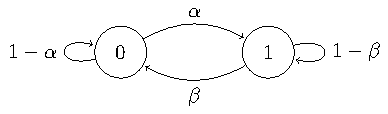
\includegraphics{math2750_files/figure-latex/twostate-1} 

}

\caption{Transition diagram for the two-state Markov chain}\label{fig:twostate}
\end{figure}

We can use this as a simple model of a broken printer, for example. If the printer is broken (state \(0\)) on one day, then with probability \(\alpha\) it will be fixed (state \(1\)) by the next day; while if it is working (state \(1\)), then with probability \(\beta\) it will have broken down (state \(0\)) by the next day.

\begin{example}
\protect\hypertarget{exm:printer}{}\label{exm:printer}

\emph{If the printer is working on Monday, what's the probability that it also is working on Wednesday?}

If we call Monday day \(n\), then Wednesday is day \(n+2\), and we want to find the two-step transition probability.
\[ p_{11}(2) = \mathbb P (X_{n+2} = 1 \mid X_n = 1) . \]
The key to calculating this is to condition on the first step again -- that is, on whether the printer is working on Tuesday. We have
\begin{align*}
  p_{11}(2) &= \mathbb P (X_{n+1} = 0 \mid X_n = 1)\,\mathbb P (X_{n+2} = 1 \mid X_{n+1} = 0) \\
  &\qquad{} + \mathbb P (X_{n+1} = 1 \mid X_n = 1)\,\mathbb P (X_{n+2} = 1 \mid X_{n+1} = 1) \\
  &= p_{10}p_{01} + p_{11}p_{11} \\
  &= \beta\alpha + (1-\beta)^2 .
\end{align*}

Another way to think of this as we summing the probabilities of all length-\(2\) paths from \(1\) to \(1\), which are \(1\to 0\to 1\) with probability \(\beta\alpha\) and \(1 \to 1 \to 1\) with probability \((1-\beta)^2\)

In the above, we used the Markov property to mean the conditional probabilities \(\mathbb P(X_{n+2} = 1 \mid X_{n+1} = k)\) did not have to depend on \(X_n\).

\end{example}

\hypertarget{n-step}{%
\subsection{\texorpdfstring{\emph{n}-step transition probabilities}{n-step transition probabilities}}\label{n-step}}

In the above example, we calculated a two-step transition probability \(p_{ij}(2) = \mathbb P (X_{n+2} = j \mid X_n = i)\) by conditioning on the first step. That is, by considering all the possible intermediate steps \(k\), we have
\[ p_{ij}(2) = \sum_{k\in\mathcal S} \mathbb P (X_{n+1} = k \mid X_n = i)\mathbb P (X_{n+2} = j \mid X_{n+1} = k) = \sum_{k\in\mathcal S} p_{ik}p_{kj} . \]

But this is exactly the formula for multiplying the matrix \(\mathsf P\) with itself! In other words, \(p_{ij}(2) = \sum_{k} p_{ik}p_{kj}\) is the \((i,j)\)th entry of the matrix \(\mathsf P^2 = \mathsf{PP}\). If we write \(\mathsf P(2) = (p_{ij}(2))\) for the matrix of two-step transition probabilities, we have \(\mathsf P(2) = \mathsf P^2\).

More generally, we see that this rule holds over multiple steps, provided we sum over all the possible paths \(i\to k_1 \to k_2 \to \cdots \to k_{n-1} \to j\) of length \(n\) from \(i\) to \(j\).

\begin{theorem}
\protect\hypertarget{thm:thm-n-step}{}\label{thm:thm-n-step}

Let \((X_n)\) be a Markov chain with state space \(\mathcal S\) and transition matrix \(\mathsf P = (p_{ij})\). For \(i,j \in \mathcal S\), write
\[ p_{ij}(n) = \mathbb P(X_n = j \mid X_0 = i) \]
for the \(n\)-step transition probability. Then
\[ p_{ij}(n) = \sum_{k_1, k_2, \dots, k_{n-1} \in \mathcal S} p_{ik_1} p_{k_1k_2} \cdots p_{k_{n-2}k_{n-1}} p_{k_{n-1}j} . \]
In particular, \(p_{ij}(n)\) is the \((i,j)\)th element of the matrix power \(\mathsf P^n\), and the matrix of \(n\)-step transition probabilities is given by \(\mathsf P(n) = \mathsf P^n\).

\end{theorem}

The so-called \textbf{Chapman--Kolmogorov equations} follow immediately from this.

\begin{theorem}[Chapman–Kolmogorov equations]
\protect\hypertarget{thm:c-k}{}\label{thm:c-k}

Let \((X_n)\) be a Markov chain with state space \(\mathcal S\) and transition matrix \(\mathsf P = (p_{ij})\). Then, for non-negative integers \(n,m\), we have
\[ p_{ij}(n+m) = \sum_{k \in \mathcal S} p_{ik}(n)p_{kj}(m) , \]
or, in matrix notation, \(\mathsf P(n+m) = \mathsf P(n)\mathsf P(m)\).

\end{theorem}

In other words, a trip of length \(n + m\) from \(i\) to \(j\) is a trip of length \(n\) from \(i\) to some other state \(k\), then a trip of length \(m\) from \(k\) back to \(j\), and this intermediate stop \(k\) can be any state, so we have to sum the probabilities.

Of course, once we know that \(\mathsf P(n) = \mathsf P^n\) is given by the matrix power, it's totally obvious that \(\mathsf P(n+m) = \mathsf P^{n+m} = \mathsf P^n \mathsf P^m = \mathsf P(n)\mathsf P(m)\).

\begin{example}
\protect\hypertarget{exm:printer2}{}\label{exm:printer2}

In our two-state broken printer example above, the matrix of two-state transition probabilities is given by
\begin{align*}
\mathsf P(2) = \mathsf P^2 &=  \begin{pmatrix} 1-\alpha & \alpha \\ \beta & 1-\beta \end{pmatrix}  \begin{pmatrix} 1-\alpha & \alpha \\ \beta & 1-\beta \end{pmatrix} \\
&=  \begin{pmatrix} (1-\alpha)^2 + \alpha\beta & (1-\alpha)\alpha + \alpha(1-\beta) \\ \beta(1-\alpha) + (1-\beta)\beta & \beta\alpha + (1-\beta)^2 \end{pmatrix} ,
\end{align*}
where the bottom right entry \(p_{11}(2)\) is what we calculated earlier.

\end{example}

One final comment. It's also convenient to consider the initial distribution \(\boldsymbol\lambda = (\lambda_i)\) as a \emph{row} vector. The first-step distribution is given by
\[ \mathbb P(X_1 = j) = \sum_{i \in \mathcal S} \lambda_i p_{ij} , \]
by conditioning on the start point.
This is exactly the \(j\)th element of the vector--matrix multiplication \(\boldsymbol\lambda \mathsf P\). More generally, the row vector of of probabilities after \(n\) steps is given by \(\boldsymbol\lambda \mathsf P^n\).

In the next section, we look at how to model some actuarial problems using Markov chains.

\hypertarget{S06-examples}{%
\section{Examples from actuarial science}\label{S06-examples}}

\begin{itemize}
\tightlist
\item
  Three Markov chain models for insurance problems
\end{itemize}

In this lecture we'll set up three simple models for an insurance company that can be analysed using ideas about Markov chains. The first example has a direct Markov chain model. For the second and third examples, we will have to be clever to find a Markov chain associated to the situation.

\hypertarget{S06-example1}{%
\subsection{A simple no-claims discount model}\label{S06-example1}}

A motor insurance company puts policy holders into three categories:

\begin{itemize}
\tightlist
\item
  no discount on premiums (state 1)
\item
  25\% discount on premiums (state 2)
\item
  50\% discount on premiums (state 3)
\end{itemize}

New policy holders start with no discount (state 1). Following a year with no insurance claims, policy holders move up one level of discount. If they start the year in state 3 and make no claim, they remain in state 3. Following a year with at least one claim, they move down one level of discount. If they start the year in state 1 and make at least one claim, they remain in state 1. The insurance company believes that probability that a motorist has a claim free year is \(\frac34\).

We can model this directly as a Markov chain:

\begin{itemize}
\tightlist
\item
  the state space \(\mathcal S = \{1,2,3\}\) is discrete, as is the time (each year);
\item
  the probability of being in a certain state at a future time is completely determined by the present state (the Markov property);
\item
  the one-step transition probabilities are not time dependent (time homogeneous).
\end{itemize}

The transition probability and transition diagram of the Markov chain are:
\[ \mathsf P = \begin{pmatrix} \frac14 & \frac34 & 0 \\ \frac14 & 0 & \frac34 \\ 0 & \frac14 & \frac34 \end{pmatrix} . \]

\begin{center}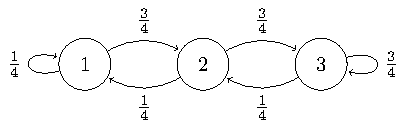
\includegraphics{math2750_files/figure-latex/example1-1} \end{center}

\begin{example}
\protect\hypertarget{exm:act1}{}\label{exm:act1}

\emph{What is the probability of having a 50\% reduction to your premium three years from now, given that you currently have no reduction on the premium?}

We want to find the three-step transition probability
\[
p_{13}(3) = \mathbb P(X_{3} = 3 \mid X_0=1) .
\]
We can find this by summing over all paths \(1 \to k_1 \to k_2 \to 3\). There are two such paths, \(1 \to 1 \to 2 \to 3\) and \(1 \to 2 \to 3 \to 3\). Thus
\[ p_{13}(3) = p_{11}p_{12}p_{23} + p_{12}p_{23}p_{33} = \frac14 \cdot\frac34 \cdot\frac34 + \frac34 \cdot\frac34 \cdot\frac34 = \frac{36}{64} = \frac{9}{16} . \]

Alternatively, we could directly calculate all the three-step transition probabilities by the matrix method, to get
\[ \mathsf P(3) = \mathsf P^3 = \mathsf{PPP} = \frac{1}{64} \begin{pmatrix} 7 & 21 & 36 \\ 7 & 12 & 45 \\ 4 & 15 & 45 \end{pmatrix} .\]
(You can check this yourself.) The desired \(p_{13}(3)\) is the top right entry \(36/64 = 9/16\).

\end{example}

\hypertarget{S06-example2}{%
\subsection{An accident model with memory}\label{S06-example2}}

According to a different model, a motorist's \(n\)th year of driving is either accident free, or has exactly one accident. (The model does not allow for more than one accident in a year.) Let \(Y_n\) be a random variable so that,
\[
Y_n=\begin{cases}
0&\text{ if the motorist has no accident in year $n$,}\\
1&\text{ if the motorist has one accident in year $n$.}
\end{cases}
\]
This defines a stochastic process \((Y_n)\) with finite state space \(\mathcal{S}=\{0,1\}\) and discrete time \(n = 1,2,3,\dots\).

The probability of an accident in year \(n+1\) is modelled as a function of the total number of previous accidents over a function of the number of years in the policy; that is,
\[
\mathbb P(Y_{n+1}= 1 \mid Y_n=y_{n},\dots ,Y_2=y_{2},Y_1=y_{1} )=\frac{f(y_1+y_2+\cdots +y_n)}{g(n)},
\]
and \(Y_{n+1} = 0\) otherwise,
where \(f\) and \(g\) are non-negative increasing functions with \(0\leq f(m)\leq g(m)\) for all \(m\).

Unfortunately \((Y_n)\) is \emph{not} a Markov chain -- it's clear that \(Y_{n+1}\) depends not only on \(Y_n\), the number accidents this year, but the entire history \(Y_1, Y_2, \dots, Y_n\).

However, we have a cunning work-around. Define \(X_n=\sum_{i=1}^n Y_i\) to be the total number of accidents up to year \(n\). Then \((X_n)\) \emph{is} a Markov chain. In fact, we have
\begin{align*}
    \mathbb P(X_{n+1}={}&{}x_{n}+1\mid X_n=x_n, \dots, X_2=x_2, X_1=x_1)\\
    &=\mathbb P(Y_{n+1}=1\mid Y_n=x_n - x_{n-1}, \dots Y_2=x_2-x_1, Y_1=x_1)\\
    &=\frac{f\big((x_n-x_{n-1}) +\cdots +(x_2-x_1) + x_1\big)}{g(n)}\\
    &=\frac{f(x_n)}{g(n)},
\end{align*}
and \(X_{n+1} = x_n\) otherwise. This clearly depends only on \(x_n\). Thus we can use Markov chain techniques on \((X_n)\) to lean about the non-Markov process \((Y_n)\)

Let's think about the conditions we placed on this model. First, the transition probabilities should lie in the range \([0,1]\). Since \(\sum_{i=1}^n y_i\leq n\), this is where we use \(0\leq f(m)\leq g(m)\). Second, the condition that \(f\) is increasing means that between drivers who have been driving the same number of years, we think the more accident-prone in the past is more likely to have an accident in the future. Third, the condition that \(g\) is increasing means that between drivers who have had the same number of accidents, we think the one who has spread those accidents over a longer period of time is less likely to have accidents in the future.

\hypertarget{S06-example3}{%
\subsection{A no-claims discount model with memory}\label{S06-example3}}

Sometimes, we are presented with a stochastic process which is not a Markov chain, but by altering the state space \(\mathcal{S}\) we can sometimes end up with a process which is a Markov chain. As such, it is important to think carefully about choice of state space. To see this we will return to the no-claims discount example.

Suppose now we have an model with four levels of discount:

\begin{itemize}
\tightlist
\item
  no discount (state 1)
\item
  20\% discount (state 2)
\item
  40\% discount (state 3)
\item
  60\% discount (state 4)
\end{itemize}

If a year is accident free, then the discount increases one level, to a maximum of 60\%. If the year has an accident, then the discount decreases, by one level if the year previous to that was accident free, but by two levels if the previous year had an accident also, to a minimum of no discount.
As before, the insurance company believes that probability that a motorist has a claim-free year is \(\frac34 = 0.75\).

We might consider the most natural example of a state space, where the states are discount levels; say, \(\mathcal{S}=\{1,2,3,4\}\). But this is not a Markov chain, since if a policy holder has an accident, we may need to know about the past in order to determine probabilities for future states, which violates the Markov property. In particular, if a motorist is in state 3 (40\% discount) and has an accident, they will either move down to level 2 (if they had not crashed the previous year, so had previously been in state 2) or to level 1 (if they had crashed the previous year, so had previously been in state 4), depending on their previous level. You can check this is the only violation of the Markov property.

However, we can be clever again, this time in the choice of our state space. Instead, we can split the 40\% level into two different states: state ``3a'' if there was an accident the previous year and state ``3b'' if there was no accident the previous year. Our states are now:

\begin{itemize}
\tightlist
\item
  no discount (state 1)
\item
  20\% discount (state 2)
\item
  40\% discount, no claim in previous year (state 3a)
\item
  40\% discount, claim in previous year (state 3b)
\item
  60\% discount (state 4)
\end{itemize}

Now this \emph{is} a Markov chain. Under the assumption of 25\% of drivers having an accident each year, the transition matrix is
\[
\mathsf P=\begin{pmatrix}
0.25 & 0.75 & 0 & 0 & 0\\
0.25 & 0 & 0.75 & 0 & 0\\
0 & 0.25 & 0 & 0 & 0.75\\
0.25 & 0 & 0 & 0 & 0.75\\
0 & 0 & 0 & 0.25 & 0.75\end{pmatrix}.
\]
The transition diagram is shown below. (Recall that we don't draw arrows with probability 0.)

\begin{center}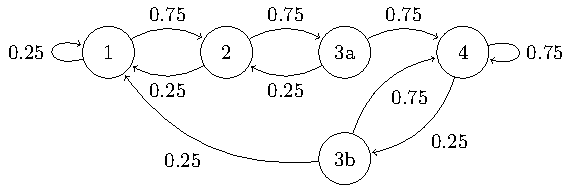
\includegraphics{math2750_files/figure-latex/example3-1} \end{center}

\textbf{In the next section}, we look at how to study large Markov chains by splitting them into smaller pieces called ``classes''.

\hypertarget{P03}{%
\section*{Problem sheet 3}\label{P03}}
\addcontentsline{toc}{section}{Problem sheet 3}

Problem Sheet 3

\hypertarget{S07-classes}{%
\section{Class structure}\label{S07-classes}}

\begin{itemize}
\tightlist
\item
  Communicating classes and irreducibility
\item
  Period of a state (and class)
\end{itemize}

\hypertarget{comm-classes}{%
\subsection{Communicating classes}\label{comm-classes}}

If we have a large complicated Markov chain, it can be useful to split the state space up into smaller pieces that can be studied separately. The idea is to split to states \(i\) and \(j\) into different pieces if we can't move from \(i\) to \(j\) and then back again after some number of steps.

\begin{definition}
\protect\hypertarget{def:comm}{}\label{def:comm}

Consider a Markov chain on a state space \(\mathcal S\) with transition matrix \(\mathsf P\). We say that state \(j\in\mathcal{S}\) is \textbf{accessible} from state \(i\in\mathcal{S}\) and write \(i \to j\) if, for some \(n\), \(p_{ij}(n)>0\).

If \(i \to j\) and \(j \to i\), we say that \(i\) \textbf{communicates with} \(j\) and write \(i \leftrightarrow j\).

\end{definition}

Here, the condition \(p_{ij}(n)>0\) means that, starting from \(i\), there's a positive chance that we'll get to \(j\) at some point in the future -- hence the term ``accessible''.

\begin{theorem}
\protect\hypertarget{thm:equiv-rel}{}\label{thm:equiv-rel}

Consider a Markov chain on a state space \(\mathcal S\) with transition matrix \(\mathsf P\). Then the ``communicates with'' relation \(\leftrightarrow\) is an \href{https://en.wikipedia.org/wiki/Equivalence_relation}{\textbf{equivalence relation}}; that is, it has the following properties:

\begin{itemize}
\tightlist
\item
  \textbf{reflexive}: \(i \leftrightarrow i\) for all \(i\);
\item
  \textbf{symmetric}: if \(i \leftrightarrow j\) then \(j \leftrightarrow i\);
\item
  \textbf{transitive}: if \(i \leftrightarrow j\) and \(j \leftrightarrow k\) then \(i \leftrightarrow k\).
\end{itemize}

\end{theorem}

\begin{proof}

\emph{Reflexivity}: Clearly \(p_{ii}(0) = 1 > 0\), because in ``zero steps'' we stay where we are. So \(i \leftrightarrow i\) for all \(i\).

\emph{Symmetry}: The definition of \(i \leftrightarrow j\) is symmetric under swapping \(i\) and \(j\).

\emph{Transitivity}. If we can get from \(i\) to \(j\) and we can get from \(j\) to \(k\), then we can get from \(i\) to \(k\) by going via \(j\). We just need to write that out formally.

Since \(i \to j\), we have \(p_{ij}(n) > 0\) for some \(n\), and since \(j \to k\), we also have \(p_{jk}(m) > 0\) for some \(m\). Then, by the Chapman--Kolmogorov equations, we have
\[ p_{ik}(n+m) = \sum_{l \in \mathcal S} p_{il}(n) p_{lk}(m) \geq p_{ij}(n) p_{jk}(m) > 0 , \]
from just picking out the \(l=j\) term in the sum. So \(i \to k\) too.

The same argument with \(k\) and \(i\) swapped gives \(k \to i\) also, so \(i \leftrightarrow k\).

\end{proof}

A fact you may remember about equivalence relations is that an equivalence relation, like \(\leftrightarrow\), partitions the space \(\mathcal S\) into \href{https://en.wikipedia.org/wiki/Equivalence_class}{\textbf{equivalence classes}}. This means that each state \(i\) is in exactly one equivalence class, and that class is the set of states \(j\) such that \(i \leftrightarrow j\). In this context, we call these \textbf{communicating classes}.

\begin{example}
\protect\hypertarget{exm:rw-class}{}\label{exm:rw-class}

In the simple random walk, provided \(p\) is not \(0\) or \(1\), every state communicates with every other state, because from \(i\) when can get to \(j > i\) by going up \(j - i\) times, and we can get to \(j < i\) by going down \(i - j\) times.. Therefore the whole state space \(\mathcal S = \mathbb Z\) is one communicating class.

\end{example}

\begin{example}
\protect\hypertarget{exm:gamblers-class}{}\label{exm:gamblers-class}

Consider the gambler's ruin Markov chain on \(\{0,1,\dots,m\}\). There are three communicating classes: \(\{0\}\) and \(\{m\}\), which don't communicate with any other states, and \(\{1,2,\dots,m-1\}\), which is like the simple random walk.

\end{example}

\begin{example}
\protect\hypertarget{exm:hsd-class}{}\label{exm:hsd-class}

Consider the following simple model for an epidemic. We have three states: healthy (H), sick (S), and dead (D). This transition matrix is
\[ \mathsf P = \begin{pmatrix} p_{\mathrm{HH}} & p_{\mathrm{HS}} & 0 \\
p_{\mathrm{SH}} & p_{\mathrm{SS}} & p_{\mathrm{SD}} \\ 0 & 0 & 1 \end{pmatrix} ,    \]
and the transition diagram is:

\begin{center}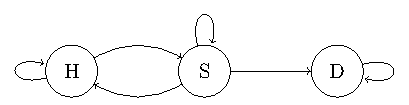
\includegraphics{math2750_files/figure-latex/HSD-1} \end{center}

Clearly H and S communicate with each other (you can become infected or recover), while D only communicates with itself (the dead do not recover). Hence, the state space \(\mathcal S = \{\mathrm{H},\mathrm{S},\mathrm{D}\}\) partitions into two communicating classes: \(\{\mathrm{H},\mathrm{S}\}\) and \(\{\mathrm{D}\}\).

\end{example}

A few more definitions that will be important later.

\begin{definition}
\protect\hypertarget{def:irreducible}{}\label{def:irreducible}

If the entire state space \(\mathcal S\) is one communicating class, we say that the Markov chain is \textbf{irreducible}.

We say that a communicating class is \textbf{closed} if no state outside the class is accessible from any state within the class. That is, class \(C \subset \mathcal S\) is closed if whenever there exist \(i \in C\) and \(j \in \mathcal S\) with \(i \to j\), then \(j \in C\) also. If a class is not closed, we say it is \textbf{open}.

If a state \(i\) is in a communicating class \(\{i\}\) by itself and that class is closed, then we say state \(i\) is \textbf{absorbing}.

\end{definition}

\begin{example}
\protect\hypertarget{exm:ex-irred}{}\label{exm:ex-irred}

Going back to the previous examples:

\begin{itemize}
\tightlist
\item
  In the simple random walk, the whole state space is one communicating class which must therefore be closed. The Markov chain has only one class, so is irreducible.
\item
  In the gambler's ruin, classes \(\{0\}\) and \(\{m\}\) are closed, because the Markov chain stays there forever, and because these closed classes consist of only one state each, \(0\) and \(m\) are absorbing states. The class \(\{1, 2, \dots, m-1\}\) is open, as we can escape the class by going to \(0\) or \(m\). The gambler's ruin chain has multiple classes, so is not irreducible.
\item
  In the ``healthy--sick--dead'' chain, the class \(\{D\}\) is closed, so D is an absorbing state, while the class \(\{H, S\}\) is open, as one can leave it by dying. The Markov chain is not irreducible.
\end{itemize}

\end{example}

\hypertarget{periodicity}{%
\subsection{Periodicity}\label{periodicity}}

When \protect\hyperlink{S02-exact-distribution}{we discussed the simple random walk, we noted} that it alternates between even-numbered and odd-numbered states. This ``periodic'' behaviour is important to understand if we want to know what will happen to the Markov chain in the future.

The idea is this: List the number of steps for all possible paths starting and ending in the state. Then the period is the \href{https://en.wikipedia.org/wiki/Greatest_common_divisor}{greatest common divisor} (or ``highest common factor'') of the integers in this list.

\begin{definition}
\protect\hypertarget{def:period}{}\label{def:period}

Consider a Markov chain with transition matrix \(\mathsf P\). We say that a state \(i\in\mathcal{S}\) has \textbf{period} \(d_i\), where
\[ d_i=\text{gcd}\big\{n\in\{1,2,\dots,\} : p_{ii}(n) > 0\big\} , \]
where gcd denotes the greatest common divisor.

If \(d_i>1\), then the state \(i\) is called \textbf{periodic}; if \(d_i = 1\), then \(i\) is called \textbf{aperiodic}.

\end{definition}

\begin{example}
\protect\hypertarget{exm:rw-period}{}\label{exm:rw-period}

Consider the simple random walk with \(p \neq 0,1\). We have \(p_{ii}(n) = 0\) for odd \(n\), since we swap from odd to even each step. But \(p_{ii}(2) = 2pq > 0\). Therefore, all states are periodic with period \(\text{gcd}\{2,4,6,\dots\} = 2\).

\end{example}

\begin{example}
\protect\hypertarget{exm:gamblers-period}{}\label{exm:gamblers-period}

For the gambler's ruin, states \(0\) and \(m\) are aperiodic (have period \(1\)), since they are absorbing states. The remaining states states \(1,2,\dots,m-1\) are periodic with period \(2\), because we swap between odd and even states, as in the simple random walk.

\end{example}

\begin{example}
\protect\hypertarget{exm:weird-period}{}\label{exm:weird-period}

Consider the Markov chain with transition diagram as shown:

\begin{center}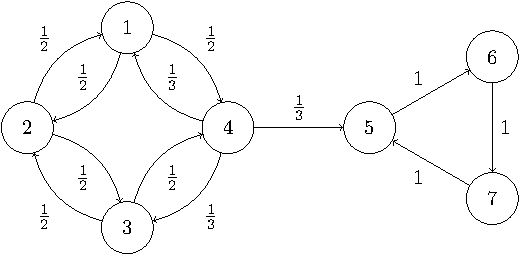
\includegraphics{math2750_files/figure-latex/periods-1} \end{center}

Importantly, we can't return from the triangle side back to the circle side. We thus see there are two communicating classes: \(\{1,2,3,4\}\), which is open, and \(\{5,6,7\}\), which is closed. The Markov chain is not irreducible, and there are no absorbing states.

The circle side swaps between odd and even states (until exiting from \(4\) to \(5\)), so states \(1\),\(2\), \(3\) and \(4\) all have period \(2\). The triangle side cycles around with certainty, meaning that states \(5\), \(6\), and \(7\) all have period \(3\).

\end{example}

You may have noticed in these examples that, within a communicating class, every state has the same period. In fact, it's always the case that states in the same class have the same period.

\begin{theorem}
\protect\hypertarget{thm:class-period}{}\label{thm:class-period}

All states in a communicating class have the same period.

Formally: Consider a Markov chain on a state space \(\mathcal S\) with transition matrix \(\mathsf P\). If \(i,j\in\mathcal S\) are such that \(i \leftrightarrow j\), then \(d_i = d_j\).

\end{theorem}

In particular, in an irreducible Markov chain, all states have the same period \(d\). We say that an irreducible Markov chain is \textbf{periodic} if \(d>1\) and \textbf{aperiodic} if \(d=1\).

\begin{proof}

Let \(i,j\) be such that \(i \leftrightarrow j\). We want to show that \(d_i = d_j\). First we'll show that \(d_i \leq d_j\), and then we'll show that \(d_j \leq d_i\), and thus conclude that they're equal.

Since \(i\leftrightarrow j\), there exist \(n,m\) such that \(p_{ij}(n)>0\) and \(p_{ji}(m)>0\). Then, by the Chapman--Kolmogorov equations,
\[ p_{ii}(n+m) =  \sum_{k \in \mathcal S} p_{ik}(n) p_{ki}(m) \geq p_{ij}(n) p_{ji}(m) > 0 .  \]
So \(d_i\) divides \(n+m\).

Let \(r\) be such that \(p_{jj}(r)>0\). Then, by the Chapman-Kolmogorov equations again,
\[
    p_{ii}(n+m+r)\geq  p_{ij}(n) p_{jj}(r) p_{ji}(m) > 0.
    \]
Hence \(d_i\) divides \(n+m+r\). But since \(d_i\) divides \(n+m\), it must be that \(d_i\) divides \(r\) also. So whenever \(p_{jj}(r)>0\), we have that \(d_i\) divides \(r\). Since \(d_i\) is a common divisor of all the \(r\)s with \(p_{jj}(r)>0\), it can't be any bigger that the \emph{greatest} common divisor of all those \(r\)s. But that greatest common divisor is by definition \(d_j\), the period of \(j\). So \(d_i \leq d_j\).

Repeating the same argument but with \(i\) and \(j\) swapped over, we get \(d_j\leq d_i\) too, and we're done.

\end{proof}

\textbf{In the next section}, we look at two problems to do with ``hitting times'': What is the probability we reach a certain state, and how long on average does it take us to get there?

\hypertarget{S08-hitting-times}{%
\section{Hitting times}\label{S08-hitting-times}}

\begin{itemize}
\tightlist
\item
  Definitions: Hitting probability, expected hitting time, return probability, expected return time
\item
  Finding these by conditioning on the first step
\item
  Return probability and expected return time for the simple random walk
\end{itemize}

\hypertarget{hitting-definitions}{%
\subsection{Hitting probability and expected hitting time}\label{hitting-definitions}}

In \protect\hyperlink{S03-gamblers-ruin}{Section 3} and \protect\hyperlink{S04-ldes}{Section 4}, we used conditioning on the first step to find the ruin probability and expected duration for the gambler's ruin problem. Here, we develop those ideas for general Markov chains.

\begin{definition}
\protect\hypertarget{def:hitting-defs}{}\label{def:hitting-defs}

Let \((X_n)\) be a Markov chain on state space \(\mathcal S\). Let \(H_{A}\) be a random variable representing the hitting time to hit a state in \(A \subset \mathcal S\), given by
\[ H_{A} = \min \{n \in \mathbb Z_+ : X_n \in A  \} . \]
The most common case we'll be interested in will be when \(A = \{j\}\) is just a single state, so
\[ H_{j} = \min \{n \in \mathbb Z_+ : X_n = j  \} . \]
(We use the convention that \(H_A = \infty\) if \(X_n \not\in A\) for all \(n\).)

The \textbf{hitting probability} \(h_{iA}\) of states \(A \subset \mathcal S\) starting from state \(i \in \mathcal S\) is
\[ h_{iA} = \mathbb P(X_n \in A \text{ for some $n \geq 0$} \mid X_0 = i) = \mathbb P(H_A < \infty \mid X_0 = i) .  \]
Again, the most common case of interest is \(h_{ij}\) the hitting probability of state \(j\) starting from state \(i\).

The \textbf{expected hitting time} \(\eta_{iA}\) of states \(A \subset \mathcal S\) starting from state \(i \in \mathcal S\) is
\[ \eta_{iA} = \mathbb E(H_A \mid X_0 = i) .  \]
Clearly \(\eta_{iA}\) can only be finite if \(h_{iA} = 1\).

\end{definition}

For the gambler's ruin problem, we found equations for hitting probabilities and expected hitting times by conditioning on the first step and solving the resulting equations. We do the same here for other Markov chains.

\begin{example}
\protect\hypertarget{exm:hitting1}{}\label{exm:hitting1}

\emph{Consider a Markov chain with transition matrix}
\[ \begin{pmatrix}
\frac15 & \frac15 & \frac15 & \frac25 \\[0.3ex]
0 & 1 & 0 & 0 \\[0.3ex]
0 & \frac12 & 0 & \frac12 \\[0.3ex]
0 & 0 & 0 & 1
\end{pmatrix} . \]
\emph{Calculate the probability that the chain is absorbed at state \(2\) when started from state \(1\).}

This is asking for the hitting probability \(h_{12}\). The key is to find simultaneous equations for all hitting probabilities \(h_{i2}\) to state 2. Clearly we have \(h_{22} = 1\), as we are already there. Also, \(h_{42} = 0\), since 4\$is an absorbing state.

For the other states, we find equations by conditioning on the first step, as we did in the gambler's ruin problem. We have
\[ h_{12} = \tfrac15 h_{12} + \tfrac15 h_{22} + \tfrac15 h_{32} + \tfrac25h_{42} \qquad \Rightarrow \qquad . \]
This is because, starting from 1, there's a \(\frac15\) probability of staying at 1; then by the Markov property it's like we're starting again from 1, so the hitting probability is still \(h_{12}\). Similarly, there's a \(\frac15\) probability of moving 2; then by the Markov property it's like we're starting again from 2, so the hitting probability is still \(h_{22}\). And so on.

We can make a similar equation for \(h_{32}\):
\[ h_{32} = \tfrac12 h_{22} + \tfrac12 h_{42} 
\]
We can simplify these two equations, using \(h_{22} = 1\) and \(h_{42} = 0\), and rearrange them, to give
\begin{align*}
\tfrac45 \tfrac45 h_{12} &= \tfrac15  + \tfrac15 h_{32}\\
h_{32} &= \tfrac12
\end{align*}
Substituting the second equation into the first, we get \(\frac45 h_{12} = \frac1{5} + \frac15\cdot\frac12 =\frac{3}{10}\), so \(h_{12} = \frac{5}{4}\,\frac{3}{10} = \frac{3}{8}\).

\end{example}

So the technique to find hitting probability \(h_{ij}\) from \(i\) to \(j\) is:

\begin{enumerate}
\def\labelenumi{\arabic{enumi}.}
\tightlist
\item
  Set up equations for all the hitting probabilities \(h_{kj}\) to \(j\) by conditioning on the first step.
\item
  Solve the resulting simultaneous equations.
\end{enumerate}

It is recommended to derive equations for hitting probabilities from first principles by conditioning on the first step. However, we can state what the general formula is: by the same conditioning method, we get
\[ h_{iA} = \begin{cases} \displaystyle\sum_{j \in \mathcal S} p_{ij} h_{jA} & \text{if $i \not\in A$} \\
1 & \text{if $i \in A$.} \end{cases} \]
It can be shown that, if these equations have multiple solutions, that the hitting probabilities are in fact the smallest non-negative solutions.

\begin{example}
\protect\hypertarget{exm:hitting2}{}\label{exm:hitting2}

\emph{Consider \protect\hyperlink{S06-example1}{the simple no-claims discount chain from Lecture 6}, which had transition matrix}
\[ \mathsf P =\begin{pmatrix}
    \tfrac14 &\tfrac34 & 0\\
    \tfrac14 &0 & \tfrac34\\
    0 &\tfrac14 & \tfrac34\\
    \end{pmatrix} .\]
\emph{Given we start in state 1 (no discount), find the expected amount of time until we reach state 3 (50\% discount).}

This question asks us to find \(\eta_{13}\). Again, we start by writing down equations for all the \(\eta_{i3}\)s. Clearly we have \(\eta_{33} = 0\).

By conditioning on the first step, we have
\begin{align*}
\eta_{13} = 1 + \tfrac14 \eta_{13} + \tfrac34 \eta_{23} \qquad &\Rightarrow \qquad \phantom{-}\tfrac34 \eta_{13} - \tfrac34\eta_{23} = 1 ,\\
\eta_{23} = 1 + \tfrac14 \eta_{13} + \tfrac34 \eta_{33} \qquad &\Rightarrow \qquad  - \tfrac14\eta_{13} + \phantom{\tfrac34}\eta_{23} = 1 .
\end{align*}
This is because the first step takes time \(1\), then we condition on what happens next.

The first equation plus three-quarters times the second gives
\[ \big(\tfrac34 - \tfrac34\tfrac14\big) \eta_{13} = \tfrac{9}{16}\eta_{13} = 1 + \tfrac34 = \tfrac 74 = \tfrac{28}{16} ,\]
which has solution \(\eta_{13} = \tfrac{28}{9} = 3.11\).

\end{example}

Similarly, if we need to, we can give a general formula
\[ \eta_{iA} = \begin{cases} 1 + \displaystyle\sum_{j \in \mathcal S} p_{ij} \eta_{jA} & \text{if $i \not\in A$} \\
0 & \text{if $i \in A$.} \end{cases} \]
Again, if we have multiple solutions, the expected hitting times are the smallest non-negative solutions.

\hypertarget{return-times}{%
\subsection{Return times}\label{return-times}}

Under the definitions above, the hitting probability and expected hitting time to a state from itself are always \(h_{ii} = 1\) and \(\eta_{ii} = 0\), as we're ``already there''.

In this case, it can be interesting to look instead at the random variable representing the \textbf{return time},
\[ M_i = \min \big\{n \in \{1,2,\dots\} : X_n = i  \big\} . \]
Note that this only considers times \(n = 1, 2, \dots\) not including \(n = 0\), so is the \emph{next} time we come back, after \(n = 0\).

We then have the \textbf{return probability} and \textbf{expected return time}
\begin{gather*} m_{i} = \mathbb P(X_n = i  \text{ for some $n \geq 1$} \mid X_0 = i) = \mathbb P(M_i < \infty \mid X_0 = i) ,  \\
 \mu_{i} = \mathbb E(M_i \mid X_0 = i) .  \end{gather*}

Just as before, we can find these by conditioning on the first step. The general equations are
\[
      m_i = \sum_{j \in \mathcal S} p_{ij}h_{ji} , \qquad
      \mu_i = 1 + \sum_{j \in \mathcal S} p_{ij}\eta_{ji},
  \]
where, if necessary, we take the minimal non-negative solution again.

\hypertarget{return-rw}{%
\subsection{Hitting and return times for the simple random walk}\label{return-rw}}

We now turn to hitting probabilities for the simple random walk, which goes up with probability \(p\) and down with probability \(q = 1-p\). This material is mandatory and is examinable, but is a bit technical; students who are struggling or have fallen behind might make a tactical decision to skip to the \protect\hyperlink{thm:rw-summary}{summary theorem at the end of the subsection} and come back to the details at a later date.

Without loss of generality, we look at \(h_{i0}\), the probability the random walk hits \(0\).
We will assume that \(i \geq 0\). For \(i < 0\), we can get the desired result by looking at the random walk in the mirror -- that is, by swapping the role of \(p\) and \(q\), and treating the positive value \(-i\).

For an initial condition, it's clear we have \(h_{00} = 1\).

For general \(i > 0\), we condition on the first step, to get
\[ h_{i0} = ph_{i+1\, 0} + qh_{i-1\, 0} .  \]
We recognise this equation from the gambler's ruin problem, and recall that we have to treat the cases \(p \neq \frac12\) and \(p = \frac12\) separately.

When \(p \neq \frac12\), the general solution is \(h_{i0} = A + B\rho^i\), where \(\rho = q/p \neq 0\), as before. The initial condition \(h_{00} = 1\) gives \(A = 1-B\), so we have a family of solutions
\[ h_{i0} = 1 + B(\rho^i - 1) . \]

In the gambler's ruin problem we had another boundary condition to find \(B\). Here we have no other conditions, but we can use the minimality condition that the hitting probabilities are the smallest non-negative solution to the equation.

When \(\rho > 1\), so \(p < \frac12\), the term \(\rho^i\) tends to infinity. Thus the minimal non-negative solution will have to take \(B = 0\), since taking \(B < 0\) would eventually give a negative solution, so \(B = 0\) gives the smallest non-negative solution. Hence the solution is \(h_{i0} = 1 + 0\rho^i = 0\), meaning we hit \(0\) with certainty. This makes sense, because for \(p < 1/2\) the random walk ``drifts'' to the left, and eventually gets back to \(0\).

When \(\rho < 1\), so \(p > \frac12\), we have that \(\rho^i - 1\) is negative and tends to \(-1\). So to get a small solution we want \(B\) as large as possible, but keeping the solution non-negative limits us to \(B \leq 1\); thus the minimality condition is achieved at \(B = 1\). The solution is \(h_{i0} = 1 + (\rho^i - 1) = \rho^i\). This is strictly less than \(1\), because for \(p > 1/2\), the random walk drifts to the right, so might drift further and further away from \(0\) and not come back.

For \(p = \frac12\), so \(\rho = 1\), we recall the general solution \(h_{i0} = A + Bi\), and the condition \(h_{00} = 1\) gives \(A = 1\). Because \(i\) is negative, to get the answer to be small we want \(B\) to be big, but non-negativity limits us to \(B \leq 0\). So the minimal non-negative solution takes \(B = 0\), so we have \(h_{i0} = 1\).

In conclusion, for \(i > 0\), the hitting probabilities are given by
\[ h_{i0} = \begin{cases} \left(\displaystyle\frac{q}{p}\right)^i & \text{if $p > \frac12$} \\ \ 1 & \text{if $p \leq \frac12$.} \end{cases} \]
(Remember that for \(i < 0\), we get the desired result by swapping the role of \(p\) and \(q\), and treating the positive value \(-i\).)

What about the return time to \(0\) (or, by symmetry, to any state \(i \in \mathbb Z\))? By conditioning on the first step, \(m_0 = ph_{1\,0} + qh_{-1\,0}\). We then have
\[ m_0 = \begin{cases} p\times 1 \hspace{0.4em}+ q\times 1 \hspace{0.4em}= 1 & \text{if $p = \frac12$} \\
p \times \displaystyle\frac qp + q\times 1 \hspace{0.4em}= 2q < 1 & \text{if $p > \frac12$} \\
p\times 1 \hspace{0.4em} + q \times \displaystyle\frac pq = 2p < 1 & \text{if $p < \frac12$.}\end{cases} \]
So for the simple symmetric random walk (\(p = \frac12\)) we have \(m_i = 1\) and are certain to return to \(0\) again and again, while for \(p \neq \frac12\), we have \(m_i < 1\) and we might never return.

One could also calculate expected hitting times \(\eta_{i0}\). For \(p \neq \frac12\), we have \(\eta_{i0} = \infty\), since \(m_0 < 1\) and we might never come back.

For \(p = \frac12\), conditioning on the first step gives the equation
\[ \eta_{i0} = 1 + \tfrac12\eta_{i+1\,0} + \tfrac12\eta_{i-1\,0} , \]
with initial condition \(\eta_{00} = 0\). This has the solution \(\eta_{i0} = -i^2 + Bi = i(B-i)\). Then non-negativity demands \(B = \infty\), as any other value would make the \(-i^2\) negative for big enough \(i\). This gives \(\eta_{i0} = \infty\), and \(\mu_0 = \infty\) also.
So for \(p = \frac12\), while the random walk always return to \(0\), it may take a very long time to do so.

In conclusion, this is what we found out:

\begin{theorem}
\protect\hypertarget{thm:rw-summary}{}\label{thm:rw-summary}

Consider the simple random walk with \(p \neq 0,1\). Then for all states \(i\) we have the following:

\begin{itemize}
\tightlist
\item
  For \(p \neq \frac12\), the return probability \(m_i\) is strictly less than 1.
\item
  For the simple symmetric random walk with \(p = \frac12\), the return probability \(m_i\) is equal to 1.
\item
  For all \(p\), the expected return time \(\mu_i\) is infinite.
\end{itemize}

\end{theorem}

\textbf{In the next section}, we look at how the return probabilities and expected return times characterise which states continue to be visited by a Markov chain in the long run.

\hypertarget{P04}{%
\section*{Problem sheet 4}\label{P04}}
\addcontentsline{toc}{section}{Problem sheet 4}

Problem Sheet 4

\hypertarget{S09-recurrence-transience}{%
\section{Recurrence and transience}\label{S09-recurrence-transience}}

\begin{itemize}
\tightlist
\item
  Definitions of recurrence and transience
\item
  Recurrence and transience as class properties
\item
  Positive and null recurrence
\end{itemize}

\hypertarget{rec-trans-def}{%
\subsection{Recurrence and transience of states}\label{rec-trans-def}}

When thinking about the long-run behaviour of Markov chains, we are interested two different types of states:

\begin{itemize}
\tightlist
\item
  \textbf{Recurrent states}, which we always keep returning to again and again;
\item
  \textbf{Transient states}, which we may return to a few times, but eventually we will leave and never come back.
\end{itemize}

The official definition is as follows; we will show that other properties follow from this.

\begin{definition}
\protect\hypertarget{def:unlabeled-div-3}{}\label{def:unlabeled-div-3}

Let \((X_n)\) be a Markov chain on a state space \(\mathcal S\). For \(i \in \mathcal S\), let \(m_i\) be the return probability
\[ m_i = \mathbb P(X_n = i \text{ for some $n \geq 1$} \mid X_0 = i) . \]
If \(m_i = 1\), we say that state \(i\) is \textbf{recurrent}; if \(m_i < 1\), we say that state \(i\) is \textbf{transient}.

\end{definition}

\begin{theorem}
\protect\hypertarget{thm:rectran}{}\label{thm:rectran}

Consider a Markov chain with transition matrix \(\mathsf P\) and state space \(\mathcal S\).

\begin{itemize}
\tightlist
\item
  If the state \(i\) is recurrent, then \(\sum_{n=1}^\infty p_{ii}(n) = \infty\), and we return to state \(i\) infinitely many times with probability \(1\).
\item
  If the state \(i\) is transient, then \(\sum_{n=1}^\infty p_{ii}(n) < \infty\), and we return to state \(i\) infinitely many times with probability \(0\).
\end{itemize}

\end{theorem}

Here \(\sum_{n=1}^\infty p_{ii}^{(n)}\) is the expected number of returns to \(i\) starting from \(i\).

We'll come to the proof in a moment, but first some examples.

\begin{example}
\protect\hypertarget{exm:rw-rec-trans}{}\label{exm:rw-rec-trans}

Consider the simple random walk. \protect\hyperlink{S08-return-rw}{In the last section} we saw that \(m_i = 1\) for the simple symmetric random walk with \(p = \frac12\), so the simple symmetric random walk is recurrent. But for \(p \neq \frac12\), we have \(m_i < 1\), so all the other simple random walks are transient.

\end{example}

\begin{example}
\protect\hypertarget{exm:rec}{}\label{exm:rec}

We saw \protect\hyperlink{periodicity}{this example in Lecture 7}:

\begin{center}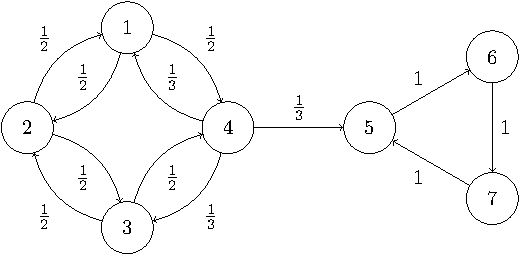
\includegraphics{math2750_files/figure-latex/periods-recap-1} \end{center}

For states 5, 6 and 7, it's clear that the return probability is 1, since the Markov chain cycles around the triangle, so these states are recurrent.

States 1, 2, 3 and 4 are recurrent. In a moment we'll see a very quick way to show this, but in the meantime we can prove it directly by getting our hands dirty.

From state 4, we might go straight to state 5, in which case we can't come back, so \(m_4 \leq 1 - p_{45} = \frac23\), and state 4 is transient. Similarly, \(m_1 \leq 1 - p_{14}p_{45} = \frac56\), because if we move from 1 to 4 to 5, we definitely won't come back to 1, so state 1 is transient. By the similar arguments, \(m_3 \leq 1 - p_{34}p_{45} = \frac56\), and \(m_2 \leq 1 - p_{21}p_{14}p_{45} = \frac{11}{12}\), so these states are both transient too.

\end{example}

Notice that the communicating class \(\{1,2,3,4\}\) is all transient, while the communicating class \(\{5,6,7\}\) is all recurrent. We shall return to this point shortly. But first, we've put off the proof for too long.

\begin{proof}[Proof of Theorem \ref{thm:rectran}]

Suppose state \(i\) is recurrent, so the probability we return to \(i\) is \(m_i = 1\). By the Markov property, we it's as if we restart the chain from \(i\), so the probability we return to \(i\) is again still \(m_i = 1\). Repeating this, we visit infinitely often with probability \(1\). In particular, the if number of visits to \(i\) starting from \(i\) is infinite, then its expectation is infinite too, and this expectation is \(\sum_{n=1}^\infty p_{ii}(n) = \infty\).

Suppose state \(i\) is transient, so the probability we return to \(i\) is \(m_i < 1\). Then the probability we return to \(i\) exactly \(r\) times before never coming back is
\[  \mathbb P \big((\text{number of returns to $i$}) = r\big) = m_i^r(1-m_i) , \]
since we must return on the first \(r\) occasions, but then fail to return any more. This is a geometric distribution \(\text{Geom}(1-m_i)\) (the version with support \(\{0,1,2,\dots\}\)). Since the expectation of a \(\text{Geom}(p)\) random variable is \((1 - p)/p\), the expected number of returns is
\[ \mathbb E(\text{number of returns to $i$}) = \sum_{n=1}^\infty p_{ii}(n)  = \frac{1 - (1 - m_i)}{1 - m_i} = \frac{m_i}{1 - m_i} . \]
This is finite, since \(m_i <1\). Since the expected number of returns is finite, the probability we return infinitely many times must be \(0\).

\end{proof}

\hypertarget{rec-tran-classes}{%
\subsection{Recurrence and transience of classes}\label{rec-tran-classes}}

We could find whether each state is transient or recurrent by calculating (or bounding) all the return probabilities \(m_i\), using the methods in \protect\hyperlink{S08-hitting-times}{the previous section}. But the following two theorems will give some highly convenient short-cuts.

\begin{theorem}
\protect\hypertarget{thm:unlabeled-div-5}{}\label{thm:unlabeled-div-5}

Within a communicating class, either every state is transient or every state is recurrent.

Formally: Let \(i, j \in \mathcal S\) be such that \(i \leftrightarrow j\). If \(i\) is recurrent, then \(j\) is recurrent also; while if \(i\) is transient, then \(j\) transient also.

\end{theorem}

For this reason, we can refer to a communicating class as a ``recurrent class'' or a ``transient class''. If a Markov chain is irreducible, we can refer to it as a ``recurrent Markov chain'' or a ``transient Markov chain''.

\begin{proof}

\emph{First part.} Suppose \(i \leftrightarrow j\) and \(i\) is recurrent. Then, for some \(m\), \(n\) we have \(p_{ij}^{(n)}\), \(p_{ji}^{(m)} > 0\). Then, by the Chapman--Kolmogorov equations,
\[ \sum_{r=1}^\infty p_{jj}^{(n+m+r)} \geq \sum_{r=1}^\infty p_{ji}^{(m)}p_{ii}^{(r)} p_{ij}^{(n)} = p_{ji}^{(m)} \left(\sum_{r=1}^\infty p_{ii}^{(r)} \right) p_{ij}^{(n)} .   \]
If \(i\) is recurrent, then \(\sum_r p_{ii}^{(r)} = \infty\). Then from the above equation, we also have \(\sum_r p_{jj}^{(n+m+r)} = \infty\), meaning \(\sum_s p_{jj}^{(s)} = \infty\), and \(j\) is recurrent.

\emph{Second part.} Suppose \(i\) is transient. Then \(j\) cannot be recurrent, because the previous argument with \(i\) and \(j\) swapped over would force \(i\) to in fact be recurrent also. So \(j\) must be transient.

\end{proof}

\begin{theorem}
\protect\hypertarget{thm:unlabeled-div-7}{}\label{thm:unlabeled-div-7}

~

\begin{itemize}
\tightlist
\item
  Every non-closed communicating class is transient.
\item
  Every finite closed communicating class is recurrent.
\end{itemize}

\end{theorem}

This theorem completely classifies the transience and recurrence of classes, with rare exception of infinite closed classes, which can require further examination.

\begin{proof}

\emph{First part.} Suppose \(i\) is in a non-closed communicating class, so for some \(j\) we have \(i \to j\), meaning \(p_{ij}^{(n)} > 0\) for some \(n\), but \(j \not\to i\), meaning that once we reach \(j\) we cannot return to \(i\). We need to show that \(i\) is transient.

The probability we return to \(i\) after time \(n\) is
\begin{align*}
\mathbb P(\text{return} & \text{ to } i \text{ after time $n$} \mid X_0 = i) \\
&= p_{ij}^{(n)}\,\mathbb P(\text{return to $i$ after time $n$} \mid X_n = j, X_0 = i) \\
&\qquad {}+ \big(1 - p_{ij}^{(n)}\big)\,\mathbb P(\text{return to $i$ after time $n$} \mid X_n \neq j, X_0 = i) \\
&\leq \mathbb P(\text{return to $i$ after time $n$} \mid X_n = j, X_0 = i) +  \big(1 - p_{ij}^{(n)}\big) \\
&\leq 0 + \big(1 - p_{ij}^{(n)}\big) \\
&< 1,
\end{align*}
since we can't get from \(j\) to \(i\), and since \(p_{ij}^{(n)} > 0\). If \(i\) were recurrent we would certainly return infinitely often, and in particular certainly return after time \(n\). So \(i\) must be transient instead.

\emph{Second part.} Suppose the class \(C\) is finite and closed. Then for some \(i \in C\), the probability that we return to \(i\) infinitely many times must be strictly positive, as we are going to stay in finitely many states of \(C\) for infinitely many time steps. Then that state \(i\) is not transient, so it must be recurrent, meaning the whole class is recurrent.

\end{proof}

Going back to the \protect\hyperlink{exm:rec}{earlier example}, we see that the class \(\{5,6,7\}\) is closed and finite, and therefore recurrent, while class \(\{1,2,3,4\}\) is not closed and therefore transient. This is much less effort than the previous method!

\hypertarget{S09-positive-null}{%
\subsection{Positive and null recurrence}\label{S09-positive-null}}

It can be useful to further divide recurrent classes, where the return probability \(m_i = 1\), by whether the expected return time \(\mu_i\) is finite or not.

\begin{definition}
\protect\hypertarget{def:unlabeled-div-9}{}\label{def:unlabeled-div-9}

Let \((X_n)\) be a Markov chain on a state space \(\mathcal S\). Let \(i \in \mathcal S\) be a recurrent state, and let \(\mu_i\) be the expected return time.
If \(\mu_i < \infty\), we say that state \(i\) is \textbf{positive recurrent}; if \(\mu_i = \infty\), we say that state \(i\) is \textbf{null recurrent}.

\end{definition}

The following facts are not difficult to prove, in a similar way to the previous results:

\begin{enumerate}
\def\labelenumi{\arabic{enumi}.}
\tightlist
\item
  In a recurrent class, either all states are positive recurrent or all states are null recurrent.
\item
  All finite closed classes are positive recurrent.
\end{enumerate}

The first result means we can refer to a ``positive recurrent class'' or a ``null recurrent class'', and an irreducible Markov chain can be a ``positive recurrent Markov chain'' or a ``null recurrent Markov chain''.

Putting everything so far together:

\begin{itemize}
\tightlist
\item
  non-closed classes are transient;
\item
  finite closed classes are positive recurrent;
\item
  infinite closed classes can be positive recurrent, null recurrent, or transient.
\end{itemize}

We know that the simple symmetric random walk is recurrent. We also saw in {[}the last section{]}((\#S08-return-rw) that \(\mu_i = \infty\), so it is null recurrent.

We can also consider the simple symmetric random walk in \(d\)-dimensions, on \(\mathbb Z^d\). At each step we pick one of the coordinates and increase or decrease it by one; each of the \(2d\) possibilities having probability \(1/(2d)\). We have seen that for \(d=1\) this is null recurrent. A famous result by the Hungarian mathematician George Pólya from 1921 states the simple symmetric random walk is null recurrent for \(d = 1\) and \(d = 2\), but is transient for \(d \geq 3\). (Perhaps this is why cars often crash into each other, but aeroplanes very rarely do?)

\hypertarget{S09-strong-markov}{%
\subsection{Strong Markov property}\label{S09-strong-markov}}

\emph{This subsection is optional and nonexaminable.}

There was a cheat somewhere in this section -- did you notice it? The last two times I lectured this course, I just hoped no one would notice -- and no one did. Still, it's a bit naughty, so in this optional and nonexaminable section, I'll come clean.

The Markov property says that, if at some fixed time \(n\) we have \(X_n = i\), then the Markov chain from that point on is just like starting all over again from the state \(i\). When we applied this in the proof of Theorem \ref{thm:rectran}, we were using as \(n\) the first return to state \(i\). But that's not a fixed time -- it's a random time. Have we messed up?

Actually we're fine. The reason is that the first return to \(i\) isn't just any old random time, it's a ``stopping time'', and the Markov property applies to stopping times too.

A stopping time is a random time where ``you know when you get there''.

\begin{definition}
\protect\hypertarget{def:stopping}{}\label{def:stopping}

Let \((X_n)\) be a stochastic process in discrete time, and let \(T\) be a random time. Then \(T\) is a \textbf{stopping time} if for all \(n\) the event \(\{T = n\}\) is determined by the random variables \(X_0, X_1, \dots, X_n\).

\end{definition}

So, for example:

\begin{itemize}
\tightlist
\item
  ``The first visit to state \(i\)'' is stopping time, because as soon as we return, we know the value of \(T\).
\item
  ``Three time-steps after the second visit to \(j\)'' is a stopping time, because after our second visit we count on three more steps and have \(T\).
\item
  ``The time-step before the first visit to \(i\)'' is not a stopping time, because we need to go one step further on to know whether or not we had just been at time \(T\).
\item
  ``The final visit to \(j\)'' is not a stopping time, because at the time of the visit we don't yet know whether we'll come back again or not.
\end{itemize}

There are lots of places in probability theory and finance when something that is true about a fixed time is also true about a random stopping time. When we use the Markov property with a stopping time, we call it the ``strong Markov property''.

\begin{theorem}[Strong Markov property]
\protect\hypertarget{thm:strong-markov}{}\label{thm:strong-markov}

Let \((X_n)\) be a Markov chain on a state space \(\mathcal S\), and let \(T\) be a stopping time that is finite with probability 1. Then all states \(x_0, \dots,x_{T-1}, i, j \in \mathcal S\) we have
\[  \mathbb P(X_{T+1}=j \mid X_T=i, X_{T-1} = x_{T-1} \dots, X_0 = x_0) = \mathbb p_{ij} . \]

\end{theorem}

\begin{proof}

We have
\begin{align*}
&\mathbb P(X_{T+1}={}x_j \mid X_T=i, X_{T-1} = x_{T-1} \dots, X_0 = x_0) \\
&\qquad{}= \sum_{n=0}^\infty \mathbb P(T = n) \mathbb P(X_{n+1}=j \mid X_n=i, X_{n-1} = x_{n-1} \dots, X_0 = x_0, T = n) \\
&\qquad{}= \sum_{n=0}^\infty \mathbb P(T = n) \mathbb P(X_{n+1}=j \mid X_n=i, X_{n-1} = x_{n-1} \dots, X_0 = x_0) \\
&\qquad{}= \sum_{n=0}^\infty \mathbb P(T = n) \mathbb P(X_{n+1}=j \mid X_n=i) \\
&\qquad{}= \sum_{n=0}^\infty \mathbb P(T = n) p_{ij}\\
&\qquad{}= p_{ij} \sum_{n=0}^\infty \mathbb P(T = n) \\
&\qquad{}= p_{ij} ,
\end{align*}
as desired. The second line was by conditioning on the value of \(T\); in the third line we deleted the superfluous conditioning \(T = n\), because \(T\) is a stopping time, so the event \(T = n\) is entirely decided by \(X_n, X_{n-1}, \dots, X_0\); the fourth line used the (usual non-strong) Markov property; the fifth line is just the definition of \(p_{ij}\); the sixth line took \(p_{ij}\) out of the sum; and the seventh line is because \(T\) is finite with probability 1, so \(\mathbb P(T = n)\) sums to 1.

\end{proof}

\hypertarget{S09-lemma}{%
\subsection{A useful lemma}\label{S09-lemma}}

\emph{This subsection is optional and nonexaminable.}

The following lemma will be used in some later optional and nonexaminable proofs.

\begin{lemma}
\protect\hypertarget{lem:lemma}{}\label{lem:lemma}

Let \((X_n)\) be an irreducible and recurrent Markov chain. Then for any initial distribution and any state \(j\), we will certainly hit \(j\), so the hitting time \(H_j\) is finite with probability 1.

\end{lemma}

\begin{proof}

It suffices to prove the lemma when the initial distribution is ``start at \(i\)''. (We can repeat for all \(i\), then build any initial distribution from a weighted sum of ``start at \(i\)''s.)

Since the chain is irreducible, we know we can get from \(i\) to \(j\), so pick \(m\) with \(p_{ji}(m) > 0\). Since the chain is recurrent, we know the return probability from \(j\) to \(j\) is 1, and we return infinitely many times with probability 1. We just need to glue these two facts together.

We have
\begin{align*}
1 &= \mathbb P(X_n = j \text{ for infinitely many $n$} \mid X_0 = j) \\
&= \mathbb P(X_n = j \text{ for some $n > m$} \mid X_0 = j) \\
&= \sum_k \mathbb P(X_m = k \mid X_0 = j) \,\mathbb P(X_n = j \text{ for some $n > m$} \mid X_m = k, X_0 = j) \\
&= \sum_k p_{jk}(m) \,\mathbb P(H_j < \infty \mid X_0 = k) ,
\end{align*}
where the last line used the Markov property to treat the chain as starting over again when it reaches some state \(k\) at time \(m\). Note that \(\sum_k p_{jk}(m) = 1\), since that's the sum of the probabilities of going anywhere in \(m\) steps. This means we must have \(\mathbb P(H_j < \infty \mid X_0 = k)\) whenever \(p_{jk}(m) > 0\), to ensure the final line does indeed sum to 1. But we stated earlier that \(p_{ji}(m) > 0\), so we indeed have \(\mathbb P(H_j < \infty \mid X_0 = i)\), as required.

\end{proof}

\textbf{In the next section}, we look at how positive recurrent Markov chains can settle into a stationary distribution and experience long-term stability.

\hypertarget{S10-stationary-distributions}{%
\section{Stationary distributions}\label{S10-stationary-distributions}}

\begin{itemize}
\tightlist
\item
  Stationary distributions and how to find them
\item
  Conditions for existence and uniqueness of the stationary distribution
\end{itemize}

\hypertarget{def-stationary-definition}{%
\subsection{Definition}\label{def-stationary-definition}}

Consider \protect\hyperlink{S05-example}{the two-state ``broken printer'' Markov chain from Lecture 5}.

\begin{center}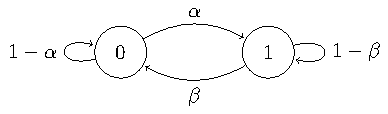
\includegraphics{math2750_files/figure-latex/twostate2-1} \end{center}

Suppose we start the chain from the initial distribution
\[ \lambda_0 = \mathbb P(X_0 = 0) = \frac{\beta}{\alpha+\beta} \qquad \lambda_1 = \mathbb P(X_0 = 1) = \frac{\alpha}{\alpha+\beta} . \]
(You may recognise this from \protect\hyperlink{P03}{Question 1 on Problem Sheet 3}.) What's the distribution after step 1? By conditioning on the initial state, we have
\begin{align*}
  \mathbb P(X_1 = 0) &= \lambda_0 p_{00} + \lambda_1 p_{10} = \frac{\beta}{\alpha+\beta}(1-\alpha) + \frac{\alpha}{\alpha+\beta}\beta = \frac{\beta}{\alpha+\beta} ,\\
  \mathbb P(X_1 = 1) &= \lambda_0 p_{01} + \lambda_1 p_{11} = \frac{\beta}{\alpha+\beta}\alpha + \frac{\alpha}{\alpha+\beta}(1-\beta) = \frac{\alpha}{\alpha+\beta} .
\end{align*}
So we're still in the same distribution we started in. By repeating the same calculation, we're still going to be in this distribution after step 2, and step 3, and forever.

More generally, if we start from a state given by a distribution \(\boldsymbol \pi = (\pi_i)\), then after step 1 the probability we're in state \(j\) is \(\sum_i \pi_i p_{ij}\). So if \(\pi_j = \sum_i \pi_i p_{ij}\), we stay in this distribution forever. In matrix form, this is \(\boldsymbol \pi = \boldsymbol \pi\mathsf P\). (Remember that \(\boldsymbol \pi\) is a \emph{row} vector.) We call such a distribution a stationary distribution.

\begin{definition}
\protect\hypertarget{def:unlabeled-div-12}{}\label{def:unlabeled-div-12}

Let \((X_n)\) be a Markov chain on a state space \(\mathcal S\) with transition matrix \(\mathsf P\).
Let \(\boldsymbol \pi = (\pi_i)\) be a distribution on \(\mathcal S\), in that \(\pi_i \geq 0\) for all \(i \in \mathcal S\) and \(\sum_{i \in \mathcal S} \pi_i = 1\). We call \(\boldsymbol \pi\) a \textbf{stationary distribution} if
\[ \pi_j = \sum_{i\in \mathcal S} \pi_i p_{ij} \quad \text{for all $j \in \mathcal S$,} \]
or, equivalently, if \(\boldsymbol \pi = \boldsymbol \pi\mathsf P\).

\end{definition}

Note that we're saying the \emph{distribution} \(\mathbb P(X_n = i)\) stays the same; the Markov chain \((X_n)\) itself will keep moving. One way to think is that if we started off a thousand Markov chains, choosing each starting position to be \(i\) with probability \(\pi_i\), then (roughly) \(1000 \pi_j\) of them would be in state \(j\) at any time in the future -- but not necessarily the same ones each time.

\hypertarget{find-stationary}{%
\subsection{Finding a stationary distribution}\label{find-stationary}}

Let's try an example. Consider \protect\hyperlink{S06-example1}{the no-claims discount Markov chain from Lecture 6} with state space \(\mathcal S=\{1,2,3\}\) and transition matrix
\[ \mathsf P =\begin{pmatrix}
    \tfrac14 &\tfrac34 & 0\\
    \tfrac14 &0 & \tfrac34\\
    0 &\tfrac14 & \tfrac34\\
    \end{pmatrix} .\]

We want to find a stationary distribution \(\boldsymbol \pi\), which must solve the equation \(\boldsymbol \pi =\boldsymbol \pi\mathsf P\), which is
\[ \begin{pmatrix} \pi_1 & \pi_2 & \pi_3 \end{pmatrix}  = \begin{pmatrix} \pi_1 & \pi_2 & \pi_3 \end{pmatrix}  \begin{pmatrix}
    \tfrac14 &\tfrac34 & 0\\
    \tfrac14 &0 & \tfrac34\\
    0 &\tfrac14 & \tfrac34\\
    \end{pmatrix} .\]

Writing out the equations coordinate at a time, we have
\begin{align*}
    \pi_1 &= \tfrac14\pi_1+\tfrac14\pi_2 , \\
    \pi_2 &= \tfrac34\pi_1+\tfrac14\pi_3 , \\
    \pi_3 &= \tfrac34\pi_2+\tfrac34\pi_3 . 
    \end{align*}
Since \(\boldsymbol\pi\) must be a distribution, we also have the ``normalising condition''
\[ \pi_1+\pi_2+\pi_3=1 . \]

The way to solve these equations is first to solve for all the variables \(\pi_i\) in terms of a convenient \(\pi_{j}\) (called the ``working variable'') and then substitute all of these expressions into the normalising condition to find a value for \(\pi_{j}\).

Let's choose \(\pi_2\) as our working variable. It turns out that \(\boldsymbol\pi = \boldsymbol\pi \mathsf{P}\) always gives one more equation than we actually need, so we can discard one of them for free. Let's get rid of the second equation, and the solve the first and third equations in terms of our working variable \(\pi_2\), to get
\begin{equation}
\pi_1=\tfrac13\pi_2 \qquad \pi_3=3\pi_2 . \label{eq:statt}
\end{equation}

Now let's turn to the normalising condition. That gives
\[ \pi_1+\pi_2+\pi_3 = \tfrac13\pi_2+\pi_2+3\pi_2 = \tfrac{13}{3} \pi_2 = 1 .\]
So the working variable is solved to be \(\pi_2 = \frac{3}{13}\). Substituting this back into \eqref{eq:statt}, we have \(\pi_1=\tfrac13\pi_2 = \frac{1}{13}\) and \(\pi_3=3\pi_2 = \frac{9}{13}\). So the full solution is
\[ \boldsymbol \pi = (\pi_1\quad \pi_2\quad \pi_3) = \left(\tfrac{1}{13}\quad \tfrac{3}{13}\quad\tfrac{9}{13}\right). \]

The method we used here can be summarised as follows:

\begin{enumerate}
\def\labelenumi{\arabic{enumi}.}
\tightlist
\item
  Write out \(\boldsymbol \pi = \boldsymbol \pi\mathsf P\) coordinate by coordinate. Discard one of the equations.
\item
  Select one of the \(\pi_i\) as a working variable and treat it as a parameter. Solve the equations in terms of the working variable.
\item
  Substitute the solution into the normalising condition to find the working variable, and hence the full solution.
\end{enumerate}

It can be good practice to use the equation discarded earlier to check that the calculated solution is indeed correct.

One extra example for further practice and to show how you should present your solutions to such problems:

\begin{example}
\protect\hypertarget{exm:stationary-1}{}\label{exm:stationary-1}

\emph{Consider a Markov chain on state space \(\mathcal S = \{1,2,3\}\) with transition matrix}
\[ \mathsf P = \begin{pmatrix} \tfrac12 & \tfrac14& \frac14 \\
                   \tfrac14& \frac12& \frac14 \\
                   0       & \frac14 & \frac34 \end{pmatrix} . \]
\emph{Find a stationary distribution for this Markov chain.}

\emph{Step 1.} Writing out \(\boldsymbol \pi = \boldsymbol \pi\mathsf P\) coordinate-wise, we have
\begin{align*}
\pi_1 &= \tfrac12 \pi_1 + \tfrac14\pi_2 \\
\pi_2 &= \tfrac14\pi_1 + \tfrac12\pi_2 + \tfrac14\pi_3 \\
\pi_3 &= \tfrac14\pi_1 + \tfrac14\pi_2 + \tfrac34\pi_3 .
\end{align*}
We choose to discard the third equation.

\emph{Step 2.} We choose \(\pi_1\) as our working variable. From the first equation we get \(\pi_2 = 2\pi_1\). From the second equation we get \(\pi_3 = 2\pi_2 - \pi_1\), and substituting the previous \(\pi_2 = 2\pi_1\) into this, we get \(\pi_3 = 3\pi_1\).

\emph{Step 3.} The normalising condition is
\[ \pi_1 + \pi_2 + \pi_3 = \pi_1 + 2\pi_1 + 3\pi_1 = 6\pi_1 = 1 . \]
Therefore \(\pi_1 = \frac16\). Substituting this into our previous expressions, we get \(\pi_2 = 2\pi_1 = \frac13\) and \(\pi_3 = 3\pi_1 = \frac12\).
Thus the solution is
\[ \boldsymbol\pi = \left( \tfrac16 \quad \tfrac13 \quad \tfrac12 \right) . \]

We can check our answer with the discarded third equation, just to make sure we didn't make any mistakes. We get
\[ \pi_3 = \tfrac14\pi_1 + \tfrac14\pi_2 + \tfrac34\pi_3 = \tfrac14\tfrac16 + \tfrac14\tfrac13+\tfrac34\tfrac12 = \tfrac1{24} + \tfrac2{24} + \tfrac{9}{24} = \tfrac{1}{2} , \]
which is as it should be.

\end{example}

\hypertarget{exist-unique}{%
\subsection{Existence and uniqueness}\label{exist-unique}}

Given a Markov chain its natural to ask:

\begin{enumerate}
\def\labelenumi{\arabic{enumi}.}
\tightlist
\item
  Does a stationary distribution exist?
\item
  If a stationary distribution does exists, is there only one, or are there be many stationary distributions?
\end{enumerate}

The answer is given by the following very important theorem.

\begin{theorem}
\protect\hypertarget{thm:statex}{}\label{thm:statex}

Consider an irreducible Markov chain.

\begin{itemize}
\tightlist
\item
  If the Markov chain is positive recurrent, then a stationary distribution \(\boldsymbol \pi\) exists, is unique, and is given by \(\pi_i = 1/\mu_{i}\), where \(\mu_{i}\) is the expected return time to state \(i\).
\item
  If the Markov chain is null recurrent or transient, then no stationary distribution exists.
\end{itemize}

\end{theorem}

We give \protect\hyperlink{stat-proof}{an optional and nonexaminable proof to the first part below}.

In our no-claims discount example, the chain is irreducible and, like all finite state irreducible chains, it is positive recurrent. Thus the stationary distribution \(\boldsymbol\pi = (\tfrac{1}{13}, \tfrac{3}{13}, \tfrac{9}{13})\) we found is the unique stationary distribution for that chain.
Once we have the stationary distribution \(\boldsymbol\pi\), we get the expected return times \(\mu_i = 1/\pi_i\) for free: the expected return times are \(\mu_1 = 13\), \(\mu_2 = \frac{13}{3} = 4.33\), and \(\mu_3 = \frac{13}{9} = 1.44\).

Note the condition in Theorem \ref{thm:statex} that the Markov chain is irreducible. What if the Markov chain is not irreducible, so has more than one communicating class? We can work out what must happen from the theorem:

\begin{itemize}
\tightlist
\item
  If none of the classes are positive recurrent, then no stationary distribution exists.
\item
  If exactly one of the classes is positive recurrent (and therefore closed), then there exists a unique stationary distribution, supported only on that closed class.
\item
  If more the one of the classes are positive recurrent, then many stationary distributions will exist.
\end{itemize}

\begin{example}
\protect\hypertarget{exm:stat-rw}{}\label{exm:stat-rw}

Consider the simple random walk with \(p \neq 0,1\). This Markov chain is irreducible, and is null recurrent for \(p = \frac12\) and transient for \(p \neq \frac12\). Either way, the theorem tells us that no stationary distribution exists.

\end{example}

\begin{example}
\protect\hypertarget{exm:stat-two}{}\label{exm:stat-two}

Consider the Markov chain with transition matrix
\[ \mathsf P = \begin{pmatrix} \frac12 & \frac12 & 0 & 0 \\
\frac12 & \frac12 & 0 & 0 \\
0 & 0 & \frac14 & \frac34\\
0 & 0 & \frac12 & \frac12\end{pmatrix} . \]
This chain has two closed positive recurrent classes, \(\{1,2\}\) and \(\{3,4\}\).

Solving \(\boldsymbol\pi = \boldsymbol\pi\mathsf P\) gives
\begin{align*}
    \pi_1 = \tfrac12 \pi_1 + \tfrac12\pi_2 \qquad &\Rightarrow \qquad \phantom{3}\pi_1 = \pi_2 \\
    \pi_2 = \tfrac12 \pi_1 + \tfrac12\pi_2 \qquad &\Rightarrow \qquad \phantom{3}\pi_1 = \pi_2 \\
    \pi_3 = \tfrac14 \pi_3 + \tfrac12\pi_4 \qquad &\Rightarrow \qquad 3\pi_3 = 2\pi_4 \\
    \pi_4 = \tfrac34 \pi_3 + \tfrac12\pi_4 \qquad &\Rightarrow \qquad 3\pi_3 = 2\pi_4 , 
\end{align*}
giving us the same two constraints twice each. We also have the normalising condition \(\pi_1 + \pi_2+\pi_3+\pi_4 = 1\). If we let \(\pi_1 + \pi_2 = \alpha\) and \(\pi_3 + \pi_4 = 1-\alpha\), we see that
\[ \boldsymbol\pi = \left(\tfrac12\alpha\quad \tfrac12\alpha\quad \tfrac25(1-\alpha)\quad \tfrac35(1-\alpha)\right) \]
is a stationary distribution for any \(0 \leq \alpha \leq 1\), so we have infinitely many stationary distributions.

\end{example}

\hypertarget{stat-proof}{%
\subsection{Proof of existence and uniqueness}\label{stat-proof}}

\emph{This subsection is optional and nonexaminable.}

It's very important to be able to find the stationary distribution(s) of a Markov chain -- you can reasonably expect a question on this to turn up on the exam. You should also know the conditions for existence and uniqueness of the stationary distribution. Being able to \emph{prove} existence and uniqueness is less important, although for completeness we will do so here.

Theorem \ref{thm:statex} had two points. The more important point was that irreducible, positive recurrent Markov chains have a stationary distribution, that it is unique, and that it is given by \(\pi_i = 1/\mu_i\). We give a proof of that below, doing the existence and uniqueness parts separately.
The less important point was that null recurrent and transitive Markov chains do not have a stationary distribution, and this is more fiddly. You can find a proof (usually in multiple parts) in books such as Norris, \href{https://www.statslab.cam.ac.uk/~james/Markov/}{\emph{Markov Chains}}, Section 1.7.

\textbf{Existence:} \emph{Every positive recurrent Markov chain has a stationary distribution.}

Before we start, one last definition. Let us call a vector \(\boldsymbol\nu\) a \textbf{stationary vector} if \(\boldsymbol\nu \mathsf P = \boldsymbol\nu\). This is exactly like a stationary distribution, except without the normalisation condition that it has to sum to 1.

\begin{proof}

Suppose that \((X_n)\) is recurrent (either positive or null, for the moment).

Our first task will be to find a stationary vector. Fix an initial state \(k\), and let \(\nu_i\) be the expected number of visits to \(i\) before we return back to \(k\). That is,
\begin{align*}
\nu_i &= \mathbb E \# \{\text{visits to $i$ before returning to $k$}\} \\
      &= \mathbb E \sum_{n=1}^{M_k} \mathbb P(X_n = i \mid X_0 = k) \\
      &= \sum_{n=1}^\infty \mathbb P(X_n = i \text{ and } n \leq M_k \mid X_0 = k)  ,
\end{align*}
where \(M_k\) is \protect\hyperlink{S08-return-times}{the return time, as in Section 8}.
Let us note for later use that, under this definition, \(\nu_k = 1\), because the only visit to \(k\) is the return to \(k\) itself.

Since \(\boldsymbol\nu\) is counting the number of visits to different states in a certain (random) time, it seems plausible that \(\boldsymbol\nu\) suitably normalised could be a stationary distribution, meaning that \(\boldsymbol\nu\) itself could be a stationary vector. Let's check.

We want to show that \(\sum_i \nu_i p_{ij} = \nu_j\). Let's see what we have:
\begin{align*}
\sum_{i \in \mathcal S} \nu_i p_{ij} &= \sum_{i \in \mathcal S} \sum_{n=1}^\infty \mathbb P(X_n = i \text{ and } n \leq M_k \mid X_0 = k) \, p_{ij} \\
&= \sum_{n=1}^\infty \sum_{i \in \mathcal S} \mathbb P(X_n = i \text{ and } X_{n+1} = j \text{ and } n \leq M_k \mid X_0 = k) \\
&= \sum_{n=1}^\infty \mathbb P(X_{n+1} = j \text{ and } n \leq M_k \mid X_0 = k) .
\end{align*}
(Exchanging the order of the sums is legitimate, because recurrence of the chain means that \(M_k\) is finite with probability 1.)
We can now do a cheeky bit of monkeying around with the index \(n\), by swapping out the visit to \(k\) at time \(M_k\) with the visit to \(k\) at time \(0\). This means instead of counting the visits from \(1\) to \(M_k\), we can count the visits from \(0\) to \(M_k - 1\). Shuffling the index about, we get
\begin{align*}
\sum_{i \in \mathcal S} \nu_i p_{ij} &= \sum_{n=0}^\infty \mathbb P(X_{n+1} = j \text{ and } n \leq M_k-1 \mid X_0 = k) \\
&= \sum_{n+1=1}^\infty \mathbb P(X_{n+1} = j \text{ and } n+1 \leq M_k \mid X_0 = k) \\
&= \sum_{n=1}^\infty \mathbb P(X_{n} = j \text{ and } n \leq M_k \mid X_0 = k) \\
&= \nu_j .
\end{align*}
So \(\boldsymbol\nu\) is indeed a stationary vector.

We now want normalise \(\boldsymbol\nu\) into a stationary distribution by dividing through by \(\sum_i \nu_i\). We can do this if \(\sum_i \nu_i\) is finite. But \(\sum_i \nu_i\) is the expected total number of visits to all states before return to \(k\), which is precisely the expected return time \(\mu_k\). Now we use assume that \((X_n)\) is \emph{positive} recurrent. This means that \(\mu_k\) is finite, so \(\boldsymbol\pi = (1/\mu_k) \boldsymbol\nu\) is a stationary distribution.

\end{proof}

\textbf{Uniqueness:} \emph{For an irreducible, positive recurrent Markov chain, the stationary distribution is unique and is given by \(\pi_i = 1/\mu_i\).}

I read the following proof in Stirzaker, \href{https://leeds.primo.exlibrisgroup.com/permalink/44LEE_INST/13rlbcs/alma991013131349705181}{\emph{Elementary Probability}}, Section 9.5.

\begin{proof}

Suppose the Markov chain is irreducible and positive recurrent, and suppose \(\boldsymbol\pi\) is a stationary distribution. We want to show that \(\pi_i = 1/\mu_i\) for all \(i\).

The only equation we have for \(\mu_k\) is \protect\hyperlink{S08-return-times}{this one from Section 8}:
\begin{equation}
\mu_k = 1 + \sum_j p_{kj} \eta_{jk} . \label{eq:pf2}
\end{equation}
Since that involves the expected hitting times \(\eta_{ik}\), let's write down \protect\hyperlink{S08-return-times}{the equation for them} too:
\begin{equation}
\eta_{ik} = 1 + \sum_j p_{ij} \eta_{jk} \qquad \text{for all $i \neq k$.} \label{eq:pf1}
\end{equation}

In order to apply the fact that \(\boldsymbol\pi\) is a stationary distribution, we'd like to get these into an equation with \(\sum_i \pi_i p_{ij}\) in it. Here's a way we can do that:
Take \eqref{eq:pf1}, multiply it by \(\pi_i\) and sum over all \(i \neq k\), to get
\begin{equation}
\sum_{i} \pi_i \eta_{ik} = \sum_{i \neq k} \pi_i + \sum_j \sum_{i \neq k} \pi_i p_{ij} \eta_{jk} . \label{eq:pf3}
\end{equation}
(The sum on the left can be over all \(i\), since \(\eta_{kk} = 0\).)
Also, take \eqref{eq:pf2} and multiply it by \(\pi_k\) to get
\begin{equation}
\pi_k \mu_k = \pi_k + \sum_j \pi_k p_{kj} \eta_{jk} \label{eq:pf4}
\end{equation}
Now add \eqref{eq:pf3} and \eqref{eq:pf4} together to get
\[
\sum_{i} \pi_i \eta_{ik} + \pi_k \mu_k = \sum_i \pi_i + \sum_j \sum_i\pi_i p_{ij} \eta_{jk} .
\]

We can now use \(\sum_i\pi_i p_{ij} = \pi_j\), along with \(\sum_i \pi_i = 1\), to get
\[ \sum_{i} \pi_i \eta_{ik} + \pi_k \mu_k = 1 + \sum_j \pi_j \eta_{jk} . \]

But the first term on the left and the last term on the right are equal, and because the Markov chain is irreducible and positive recurrent, they are finite. (That was \protect\hyperlink{S09-lemma}{our lemma in the previous section}.) Thus we're allowed to subtract them, and we get \(\pi_k \mu_k = 1\), which is indeed \(\pi_k = 1/\mu_k\). We can repeat the argument for every choice of \(k\).

\end{proof}

\textbf{In the next section}, we see how the stationary distribution tells us very important things about the long-term behaviour of a Markov chain.

\hypertarget{P05}{%
\section*{Problem sheet 5}\label{P05}}
\addcontentsline{toc}{section}{Problem sheet 5}

Problem Sheet 5

\hypertarget{S11-long-term-chains}{%
\section{Long-term behaviour of Markov chains}\label{S11-long-term-chains}}

\begin{itemize}
\tightlist
\item
  The limit theorem: convergence to the stationary distribution for irreducible, aperiodic, positive recurrent Markov chains
\item
  The ergodic theorem for the long-run proportion of time spent in each state
\end{itemize}

\hypertarget{equilibrium}{%
\subsection{Convergence to equilibrium}\label{equilibrium}}

In this section we're interested in what happens to a Markov chain \((X_n)\) in the long-run -- that is, when \(n\) tends to infinity.

One thing that \emph{could} happen over time is that the distribution \(\boldsymbol\lambda \mathsf P^n\) of the Markov chain could gradually settle down towards some ``equilibrium distribution''. Further, perhaps that long-term equilibrium might not depend on the initial distribution, but the initial behaviour might eventually almost disappear, exhibiting a ``lack of memory'' of the start of the process.

Just in case that does happen, let's give it a name.

\begin{definition}
\protect\hypertarget{def:eq-dist}{}\label{def:eq-dist}

Let \((X_n)\) be a Markov chain on a state space \(\mathcal S\) with transition matrix \(\mathsf P\). Suppose there exists a distribution \(\mathbf p^* = (p_i^*)\) on \(\mathcal S\) (so \(p_i^* \geq 0\) and \(\sum_i p_i^* = 1\)) such that, whatever the initial distribution \(\boldsymbol\lambda = (\lambda_i)\), we have \(\mathbb P(X_n = j) \to p^*_j\) as \(n \to \infty\) for all \(j \in \mathcal S\). Then we say that \(\mathbf p^*\) is an \textbf{equilibrium distribution}.

\end{definition}

It's clear there can only be at most one equilibrium distribution -- but will there be one at all? The following is the most important result in this course. (Recall that an irreducible Markov chain is aperiodic if it has period \(1\).)

\begin{theorem}[Limit theorem]
\protect\hypertarget{thm:limit}{}\label{thm:limit}

Let \((X_n)\) be an irreducible and aperiodic Markov chain. Then for any initial distribution \(\boldsymbol\lambda\), we have that \(\mathbb P(X_n = j) \to 1/\mu_j\) as \(n \to \infty\), where \(\mu_j\) is the expected return time to state \(j\).

In particular:

\begin{itemize}
\tightlist
\item
  Suppose \((X_n)\) is positive recurrent. Then the unique stationary distribution \(\boldsymbol\pi\) given by \(\pi_j = 1/\mu_j\) is the equilibrium distribution, so \(\mathbb P(X_n = j) \to \pi_j\) for all \(j\).
\item
  Suppose \((X_n)\) is null recurrent or transient. Then \(\mathbb P(X_n = j) \to 0\) for all \(j\), and there is no equilibrium distribution.
\end{itemize}

\end{theorem}

I particularly like how this one theorem gathers together all the ideas from the course in one result (Markov chains, irreducibility, periodicity, recurrence/transience, positive/null recurrence, return times, stationary distributions\ldots).

Note the three conditions for convergence to an equilibrium distribution: irreducibility, aperiodicity, and positive recurrence.

Consider a irreducible, aperiodic, positive recurrent Markov chain. Taking the initial distribution to be starting in state \(i\) with certainty, the limit theorem tells us that \(p_{ij}(n) \to \pi_j\) for all \(i\) and \(j\). This means that the \(n\)-step transition matrix will have the limiting value
\[ \lim_{n \to \infty} \mathsf P(n) = \begin{pmatrix}
     \pi_1 & \pi_2 & \cdots & \pi_N \\
     \pi_1 & \pi_2 & \cdots & \pi_N \\
     \vdots & \vdots & \vdots & \vdots \\
     \pi_1 & \pi_2 & \cdots & \pi_N \end{pmatrix} , \]
where each row is identical.

We give an \protect\hyperlink{S11-proofs}{full proof of the limit theorem} below (optional and nonexaminable). However, this result gets part way there and is straightforward.

\begin{theorem}
\protect\hypertarget{thm:unlabeled-div-15}{}\label{thm:unlabeled-div-15}

If an equilibrium distribution \(\mathbf p^*\) does exist, then \(\mathbf p^*\) is a stationary distribution.

\end{theorem}

Given this result it's clear that an irreducible Markov chain cannot have an equilibrium distribution if it is null recurrent or transient, as it doesn't even have a stationary distribution. So the positive recurrent case is the hard (nonexaminable) one.

\begin{proof}

We need to verify that \(\mathbf p^* \mathsf P = \mathbf p^*\). We have
\[ \sum_i p_i^* p_{ij} = \sum_i \left(\lim_{n\to\infty} p_{ki}(n) \right) p_{ij} = \lim_{n\to\infty} \sum_i p_{ki}(n) p_{ij} = \lim_{n\to\infty} p_{kj}(n+1) = p^*_j , \]
as desired.

\end{proof}

(Strictly speaking, swapping the sum and the limit is only formally justified when the state space is finite, although the theorem is true universally.)

\hypertarget{convergence-examples}{%
\subsection{Examples of convergence and non-convergence}\label{convergence-examples}}

\begin{example}
\protect\hypertarget{exm:conv1}{}\label{exm:conv1}

\protect\hyperlink{S05-example}{The two-state ``broken printer'' Markov chain} is irreducible, aperiodic, and positive recurrent, so its stationary distribution is also the equilibrium distribution. We proved this from first principles in \protect\hyperlink{P03}{Question 1 on Problem Sheet 3}.

\end{example}

\begin{example}
\protect\hypertarget{exm:conv2}{}\label{exm:conv2}

Recall \protect\hyperlink{S06-example1}{the simple no-claims discount Markov chain from Lecture 6}, which is irreducible, aperiodic, and positive recurrent. We saw last time that is has the unique stationary distribution
\[ \boldsymbol\pi = \left(\tfrac1{13} \quad \tfrac{3}{13}\quad \tfrac9{13}\right) = (0.0769\quad 0.2308\quad 0.6923) . \]

From the limit theorem, we see that the \(n\)-step transition probability tends to a limit where every row is equal to \(\boldsymbol\pi\). We can check using a computer: for \(n = 12\), say,
\[ \mathsf P(12) = \mathsf P^{12} = \begin{pmatrix} 0.0770 & 0.2308 & 0.6923 \\ 0.0769 & 0.2308 & 0.6923 \\ 0.0769 & 0.2308 & 0.6923 \end{pmatrix}, \]
where \(p_{ij}(12)\) is equal to \(\pi_j\) up to at least 3 decimal places for all \(i,j\).

\end{example}

\begin{example}
\protect\hypertarget{exm:conv-rw}{}\label{exm:conv-rw}

The simple random walk is null recurrent for \(p = \frac12\) and transient otherwise. Either way, we have \(\mathbb P(X_n = i) \to 0\) for all states \(i\), and there is no equilibrium distribution.

\end{example}

\begin{example}
\protect\hypertarget{exm:conv4}{}\label{exm:conv4}

Consider a Markov chain \((X_n)\) on state space \(\mathcal S = \{0,1\}\) and transition matrix
\[ \mathsf P = \begin{pmatrix} 0 & 1 \\ 1 & 0 \end{pmatrix} . \]
So at each stage we swap from state \(0\) to state \(1\) and back again. This chain is irreducible and positive recurrent, so it has a unique stationary distribution, which is clearly \(\boldsymbol\pi = (\frac12\quad\frac12)\).

However, we don't have convergence to equilibrium. If we start from initial distribution \((\lambda_0, \lambda_1)\), then \(\mathbb P(X_n = 0) = \lambda_0\) for even \(n\) and \(\mathbb P(X_n = 0) = \lambda_1\) for odd \(n\). When \(\lambda_0 \neq \frac12\), this does not converge.

The point is that this chain is \emph{not} aperiodic: it has period \(2\), so the limit theorem does not apply.

\end{example}

\begin{example}
\protect\hypertarget{exm:conv5}{}\label{exm:conv5}

Consider a Markov chain with state space \(\mathcal S = \{1,2,3\}\) and transition diagram as shown below.

\begin{center}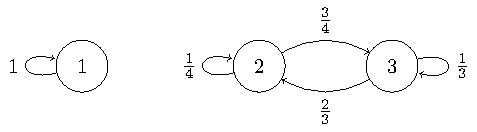
\includegraphics{math2750_files/figure-latex/stat-ex-1} \end{center}

This chain is not irreducible, but has two aperiodic and positive recurrent communicating classes. In particular, it has many stationary distributions including \((1, 0, 0)\) and \((0, \frac8{17}, \frac9{17})\) (optional exercise for the reader). If we start in state 1, then the limiting distribution is the former, while if we start in states 2 or 3, the limiting distribution is the latter.

In particular, as \(n \to \infty\), we have
\[ \mathsf P^{(n)} \to \begin{pmatrix} 1 & 0 & 0 \\ 0 & \frac8{17} & \frac9{17} \\ 0 & \frac8{17} & \frac9{17} \end{pmatrix}. \]

\end{example}

\hypertarget{S11-ergodic}{%
\subsection{Ergodic theorem}\label{S11-ergodic}}

The limit theorem looked at the limit of \(\mathbb P(X_n = j)\), the probability that the Markov chain is in state \(j\) at some specific point in time \(n\) a long time in the future. We could also look at the \emph{long-run amount of time} spent in state \(j\); that is, averaging the behaviour over a long time period. (The word ``ergodic'' is used in mathematics to refer to concepts to do with the long-term proportion of time.)

Let us write
\[ V_j(N) := \# \big\{ n < N : X_n = j \} \]
for the total number of visits to state \(j\) up to time \(N\). Then we can interpret \(V_j(n)/n\) as the proportion of time up to time \(n\) spent in state \(j\), and its limiting value (if it exists) to be the \textbf{long-run proportion of time} spent in state \(j\).

\begin{theorem}[Ergodic theorem]
\protect\hypertarget{thm:ergodic}{}\label{thm:ergodic}

Let \((X_n)\) be an irreducible Markov chain. Then for any initial distribution \(\boldsymbol\lambda\) we have that \(V_j(n)/n \to 1/\mu_j\) almost surely as \(n \to \infty\), where \(\mu_j\) is the expected return time to state \(j\).

In particular:

\begin{itemize}
\tightlist
\item
  Suppose \((X_n)\) is positive recurrent. Then there is a unique stationary distribution \(\boldsymbol\pi\) given by \(\pi_j = 1/\mu_j\), and \(V_j(n)/n \to \pi_j\) almost surely for all \(j\).
\item
  Suppose \((X_n)\) is null recurrent or transient. Then \(V_j(n)/n \to 0\) almost surely for all \(j\).
\end{itemize}

\end{theorem}

For completeness, we should note that ``almost sure'' convergence means that \(\mathbb P(V_j(n)/n \to 1/\mu_j) = 1\), although the precise definition is not important for us in this module.

Note that, because we are averaging over a long-time period, we no longer need the condition that the Markov chain is aperiodic. For converge of the long-term proportion of time to the stationary distribution we just need irreducibility and positive recurrence.

Again, we give an optional and nonexaminable proof \protect\hyperlink{S11-proofs}{below}.

\begin{example}
\protect\hypertarget{exm:ergodic-ex}{}\label{exm:ergodic-ex}

Recall \protect\hyperlink{S06-example1}{the simple no-claims discount Markov chain}. Since this chain is irreducible and positive recurrent, we now see that the long-term proportion of time spent in each state corresponds to the stationary distribution \(\boldsymbol\pi = (\frac1{13} \quad \frac{3}{13}\quad \frac9{13})\). Therefore, over the lifetime of an insurance policy held for a long period of time, the average discount is approximately
\[ \tfrac{1}{13}(0\%) + \tfrac{3}{13}(25\%) + \tfrac{9}{13}(50\%) = \tfrac{21}{52} = 40.4\% . \]

\end{example}

\begin{example}
\protect\hypertarget{exm:ergodic-ex2}{}\label{exm:ergodic-ex2}

The two-state ``swapping'' chain we saw earlier did have a unique stationary distribution \((\frac12, \frac12)\), but did not have an equilibrium distribution, because it was periodic. But it is true that \(V_0(n)/n \to \pi_0 = \frac12\) and \(V_1(n)/n \to \pi_! = \frac12\), due to the ergodic theorem. So although where we are at some specific point in the future depends on where started from, in the long run we always spend half our time in each state.

\end{example}

\hypertarget{S11-proofs}{%
\subsection{Proofs of the limit and ergodic theorems}\label{S11-proofs}}

\emph{This subsection is optional and nonexaminable.}

Again, it's important to be able to use the limit and ergodic theorems, but less important to be able to prove them.

First, the limit theorem. The only bit left is the first part: that for an irreducible, aperiodic, positive recurrent Markov chain, the stationary distribution \(\boldsymbol\pi\) is an equilibrium distribution.

This cunning proof uses a technique called ``coupling''. When looking at two different random objects \(X\) and \(Y\) (like random variables or stochastic processes), it seems natural to prefer \(X\) and \(Y\) to be independent. However, \textbf{coupling} is the idea that it can sometimes be beneficial to let \(X\) and \(Y\) actually be dependent on each other.

\begin{proof}[Proof of Theorem \ref{thm:limit}]

Let \((X_n)\) be our irreducible, aperiodic, positive recurrent Markov chain with transition matrix \(\mathsf P\) and initial distribution \(\boldsymbol\lambda\). Let \((Y_n)\) be a Markov chain also with transition matrix \(\mathsf P\) but ``in equilibrium'' -- that is, started from the stationary distribution \(\boldsymbol\pi\), and thus staying in that distribution for ever.

Pick a state \(s \in \mathcal S\), and let \(T\) be the first time the \(X_n = Y_n = s\) (or \(T = \infty\), if that never happens). Now here's the coupling: after \(T\), when \((X_n)\) and \((Y_n)\) collide at \(s\), then make \((X_n)\) stick to \((Y_n)\), so \(X_n = Y_n\) for \(n \geq T\). Since a Markov chain has no memory, \((X_{T+n}) = (Y_{T+n})\) is still just a Markov chain with the same transition probabilities from that point on. (Readers of \protect\hyperlink{S09-strong-markov}{a previous optional subsection} will recognise \(T\) as a stopping time and will notice we're using the strong Markov property.) Most importantly, thanks to the coupling, from the time \(T\) onwards, \((X_n)\) will also always have distribution \(\boldsymbol\pi\), a fact that will obviously be very useful in this proof.

It will be important that \(T\) is finite with probability 1. Define \((\mathbf Z_n)\) by \(\mathbf Z_n = (X_n, Y_n)\). So \((\mathbf Z_n)\) is a Markov chain on \(\mathcal S \times \mathcal S\), and \(T\) is the expected hitting time of \((\mathbf Z_n)\) to the state \((s, s) \in \mathcal S \times \mathcal S\). The transition probabilities for \((\mathbf Z_n)\) are \(\mathsf{\tilde P} = (\tilde p_{(i,k)(j,l)})\) where
\[ \tilde p_{(i,k)(j,l)} = p_{ij}p_{kl} . \]
This is the probability that the joint chain goes from \(\mathbf Z_n = (X_n, Y_n) = (i, k)\) to \(\mathbf Z_{n+1} = (X_{n+1}, Y_{n+1}) = (j, l)\).

Since the original Markov chain is irreducible and aperiodic, this means that \(p_{ij}(n), p_{kl}(n) > 0\) for all \(n\) sufficiently large, so \(\tilde p_{(i,k)(j,l)}(n) > 0\) for all \(n\) sufficiently large also, meaning that \((\mathbf Z_n)\) is irreducible (and, although this isn't required, aperiodic). Further, \((\mathbf Z_n)\) has a stationary distribution \(\mathbf{\tilde \pi} = (\tilde \pi_{(i,k)})\) where
\[ \tilde \pi_{(i,k)} = \pi_i \pi_k , \]
which means that \((\mathbf Z_n)\) is positive recurrent. Thus \(T\) is finite with probability 1.

So we can finally prove the limit theorem. We want to show that \(\mathbb P(X_n = i)\) tends to \(\pi_i\). The difference between them is
\begin{align*}
\big|\mathbb P(X_i = i) - \pi_i\big|
&= \mathbb P(n \leq T)\times\big|\mathbb P(X_i = i \mid n \leq T) - \pi_i\big|  + P(n > T) \times |\pi_i - \pi_i| \\
&= \mathbb P(n \leq T)\times\big|\mathbb P(X_i = i \mid n \leq T) \\
&\leq \mathbb P(n \leq T) .
\end{align*}
Here, the equality on the first line is because \((X_n)\) follows the stationary distribution exactly once it sticks to \((Y_n)\) after time \(T\), and the inequality on the third line is because the absolute difference between two probabilities is between 0 and 1. But we've already shown that \(T\) is finite with probability 1, so \(\mathbb P(n \leq T) = \mathbb P(T \geq n) \to 0\), and we're done.

\end{proof}

The proof of the ergodic theorem uses the law of large numbers. Recall that the law of large numbers states that if \(Y_1, Y_2, \dots\) are IID random variables with mean \(\mu\), then
\[ \frac{Y_1 + Y_2 + \cdots + Y_n}{n} \to \mu \qquad \text{as $n \to \infty$}. \]
This means it's also true that for any sequence \((a_n)\) with \(a_n \to \infty\), we also have
\[ \frac{Y_1 + Y_2 + \cdots + Y_{a_n}}{a_n} \to \mu \qquad \text{as $n \to \infty$}. \]

\begin{proof}[Proof of Theorem \ref{thm:ergodic}]

If \((X_n)\) is transient, then the number of visits to state \(i\) is finite with probability 1, so \(V_i(n)/n \to 0\), as required.

Suppose instead that \((X_n)\) is recurrent. By our \protect\hyperlink{S09-lemma}{useful lemma} we know we will hit \(i\) in finite time, so we can ignore that negligible ``burn-in'' period, and (by the strong Markov property) assume we start from \(i\). Let \(M_{i}^{(r)}\) be the time between the \(r\)th and \((r+1)\)th visits to \(i\). Note that the \(M_{i}^{(r)}\) are IID with mean \(\mu_i\).

The time of the last visit to \(i\) before time \(n\) is
\[ M_{i}^{(1)} + M_{i}^{(2)} + \cdots + M_{i}^{(V_i(n)-1)} < n ,\]
and the time of the first visit to \(i\) after time \(n\) is
\[ M_{i}^{(1)} + M_{i}^{(2)} + \cdots + M_{i}^{(V_i(n))} \geq n .\]
Hence
\begin{equation}
\frac{M_{i}^{(1)} + M_{i}^{(2)} + \cdots + M_{i}^{(V_i(n)-1)}}{V_i(n)} < \frac{n}{V_i(n)} \leq \frac{M_{i}^{(1)} + M_{i}^{(2)} + \cdots + M_{i}^{(V_i(n))}}{V_i(n)} . \label{eq:erg}
\end{equation}

Because \((X_n)\) is recurrent, we keep returning to \(i\), so \(V_i(n) \to \infty\) with probability 1. Hence, by the law of large numbers, both the left- and right-hand sides of \eqref{eq:erg} tend to \(\mathbb E M_{i}^{(r)} = \mu_i\). So \(n/V_i(n)\) is sandwiched between them, and tends to \(\mu_i\) too. Finally \(n/V_i(n) \to \mu_i\) is equivalent to \(V_i(n)/n \to 1/\mu_i\), so we are done.

\end{proof}

This completes the material on discrete time Markov chains. \textbf{In the next section}, we recap what we have learned, and have a little time for some revision.

\hypertarget{S11-revision-i}{%
\section{Revision of Part 1: Discrete time Markov chains}\label{S11-revision-i}}

\begin{itemize}
\tightlist
\item
  No new material in this section, but a half-week break to catch up and revise what we've learned
\end{itemize}

\hypertarget{S12-revision}{%
\subsection{Things to do}\label{S12-revision}}

We've now finished the material of the Part 1 of the module, on discrete time Markov chains. So this is a good time to take stock, revise what we've learned, and make sure we're completely up to date before starting Part 2 of the module on continuous time processes.

Some things you may want to do in lieu of reading a section of notes:

\begin{itemize}
\tightlist
\item
  Make sure you've completed \textbf{Problem Sheets 1 to 6}, and go back to any questions that stumped you before.
\item
  Start working on \textbf{\protect\hyperlink{A2}{Assessment 2}} which is due on ?????? ??? (Week 8).
\item
  Start working on \textbf{\protect\hyperlink{computer}{Computer Practical 2}} (which doubles as Assessment 3). There are optional computer drop-in sessions in Week 7, and the work is due on ????? ???? (Week 9).
\item
  Re-read any sections of notes you struggled with earlier.
\item
  Take the opportunity to look at the optional non-examinable subsections if you opted out the first time around. (\protect\hyperlink{S09-strong-markov}{Section 9}, \protect\hyperlink{S10-proof}{Section 10}, \protect\hyperlink{S11-proofs}{Section 11})
\item
  \href{mailto:m.aldridge@leeds.ac.uk}{Let me know} if there's anything from this part of the course you'd like me to go through in next week's lecture.
\end{itemize}

\hypertarget{S12-summary-i}{%
\subsection{Summary of Part 1}\label{S12-summary-i}}

The following list is not exhaustive, but if you can do most of the things on the list, you're well placed for the exam.

\begin{itemize}
\item
  Define the simple random walk and other random walks.
\item
  Perform elementary calculations for the simple random walk, including by referring to the exact binomial distribution.
\item
  Calculate the expectation and variance of general random walks.
\item
  Define the gambler's ruin Markov chain.
\item
  Find the ruin probability and expected duration for the gambler's ruin by (i) setting up equations by conditioning on the first step and (ii) solving the resulting linear difference equation.
\item
  Draw a transition diagram of a Markov chain given the transition matrix
\item
  Calculate \(n\)-step transitions probabilities by (a) summing the probabilities over all relevant paths or (b) calculating the matrix power
\item
  Find the communicating classes in a Markov chain.
\item
  Calculate the period of communicating class,
\item
  Calculate hitting probabilities and expected hitting times by (i) setting up equations by conditioning on the first step and (ii) solving the resulting simultaneous equations
\item
  Define positive recurrence, null recurrence and transience, and explain their properties
\item
  Find the positive recurrence, null recurrence or transience of communicating classes
\item
  Find the stationary distribution of Markov chain
\item
  Give conditions for a stationary distribution to exist and be unique
\item
  Give conditions for convergence to an equilibrium distribution
\item
  Calculate long-term proportions of time using the ergodic theorem
\end{itemize}

\textbf{In the next section}, we begin our study of continuous time Markov processes by looking at the most important example: the Poisson process.

\hypertarget{part-part-ii-continuous-time-markov-jump-processes}{%
\part*{Part II: Continuous time Markov jump processes}\label{part-part-ii-continuous-time-markov-jump-processes}}
\addcontentsline{toc}{part}{Part II: Continuous time Markov jump processes}

\hypertarget{S13-poisson-poisson}{%
\section{Poisson process with Poisson increments}\label{S13-poisson-poisson}}

\begin{itemize}
\tightlist
\item
  Reminder: the Poisson distribution
\item
  The Poisson process has independent Poisson increments
\item
  Summed and marked Poisson processes
\end{itemize}

\newcommand{\Po}{\operatorname{Po}}
\newcommand{\ee}{\mathrm{e}}

\hypertarget{poisson-dist}{%
\subsection{Poisson distribution}\label{poisson-dist}}

In the next three sections we'll be considering the Poisson process, a continuous time discrete space process with the Markov property. Given its name, it's not surprising to hear the Poisson \emph{process} is related to the Poisson \emph{distribution}. Let's start with a reminder of that.

Recall that a discrete random variable \(X\) has a \textbf{Poisson distribution} with rate \(\lambda\), written \(X \sim \operatorname{Po}(\lambda)\), if its probability mass function is
\[ \mathbb P(X = n) = \mathrm{e}^{-\lambda} \frac{\lambda^n}{n!} \qquad n = 0,1,2,\dots. \]

The Poisson distribution is often used to model the number of ``arrivals'' in a fixed amount of time -- for example, the number of calls to a call centre in one hour, the number of claims to an insurance company in one year, or the number of particles decaying from a large amount of radioactive material in one second.

The Poisson distribution is named after the French mathematician and physicist Siméon Denis Poisson, who studied it in 1837, although it was used by another French mathematician, Abraham de Moivre, more than 100 years earlier.

Recall the following facts about of the Poisson distribution:

\begin{enumerate}
\def\labelenumi{\arabic{enumi}.}
\tightlist
\item
  Its expectation is \(\mathbb EX = \lambda\) and the variance is \(\operatorname{Var}(X) = \lambda\).
\item
  If \(X \sim \operatorname{Po}(\lambda)\) and \(Y \sim \operatorname{Po}(\mu)\) are independent, then \(X + Y \sim \operatorname{Po}(\lambda+\mu)\).
\item
  Let \(X \sim \operatorname{Po}(\lambda)\) represent some arrivals, and independently ``mark'' each arrival with probability \(p\). Then the number of marked arrivals \(Y\) has distribution \(Y = \operatorname{Po}(p\lambda)\), the number of unmarked arrivals \(Z\) has distribution \(Z \sim \operatorname{Po}((1-p)\lambda)\), and \(Y\) and \(Z\) are independent.
\end{enumerate}

(When mathematicians say ``recall'' usually they mean ``remember this well-known fact you've been taught before'', but sometimes they secretly mean ``I'm going to tell you something you probably haven't seen before, but I can't be bothered to prove it''. Fact number 3 might be more of the latter kind\ldots)

\hypertarget{poisson-def-poisson}{%
\subsection{Definition 1: Poisson increments}\label{poisson-def-poisson}}

Suppose that, instead of just modelling the number of arrivals in a \emph{fixed} amount of time, we want to continually model the total number of arrivals as it changes over time. This will be a stochastic process with discrete state space \(\mathcal S = \mathbb Z_+ = \{0,1,2,\dots\}\) and continuous time \(\mathbb R_+ = [0,\infty)\). In continuous time, we will normally write stochastic processes as \((X(t))\), with the time variable being a \(t\) in brackets, rather than a subscript \(n\) as we had in discrete time.

Suppose calls arrive at a call centre at a rate of \(\lambda = 100\) an hour. The following assumptions seem reasonable:

\begin{itemize}
\tightlist
\item
  We begin counting with \(X(0) = 0\) calls.
\item
  The number of calls in the first hour is \(X(1) \sim \operatorname{Po}(100)\). The number of calls in the second hour \(X(2) - X(1)\) will also be \(\operatorname{Po}(100)\), and will be independent of the number of calls in the first hour.
\item
  The number of calls in a two hour period will be \(X(t+2) - X(t) \sim \operatorname{Po}(200)\), while the number of calls in a half-hour period will be \(X(t+\frac12) - X(t) \sim \operatorname{Po}(50)\).
\end{itemize}

These properties will define the Poisson process.

\begin{definition}
\protect\hypertarget{def:poisson-def-1}{}\label{def:poisson-def-1}

The \textbf{Poisson process} with rate \(\lambda\) is defined as followed. It is a stochastic process \((X(t))\) with continuous time \(t \in [0,\infty)\) and discrete state space \(\mathcal S = \mathbb Z_+\) with the following properties:

\begin{enumerate}
\def\labelenumi{\arabic{enumi}.}
\tightlist
\item
  \(X(0) = 0\);
\item
  Poisson increments: \(X(t+s) - X(t) \sim \operatorname{Po}(\lambda s)\) for all \(s,t>0\);
\item
  independent increments: \(X(t_2) - X(t_1)\) and \(X(t_4) - X(t_3)\) are independent for all \(t_1 \leq t_2 \leq t_3 \leq t_4\).
\end{enumerate}

\end{definition}

Note that the condition \(t_1 \leq t_2 \leq t_3 \leq t_4\) means that the time interval from \(t_1\) to \(t_2\) and the time interval from \(t_3\) to \(t_4\) don't overlap. (Overlapping time intervals will not have independent increments, as arrivals in the overlap will count for both.)

The Poisson process was discovered in the first decade 20th century, and the process was named after the distribution. Many people were working on similar things, so it's difficult to say who discovered it first, but important work was done by the Swedish actuary and mathematician Filip Lundberg and the Danish engineer and mathematician AK Erlang,

\begin{example}
\protect\hypertarget{exm:poisson-ex-1}{}\label{exm:poisson-ex-1}

\emph{Claims arrive at insurance company at a rate of \(\lambda = 8\) per hour, modelled as a Poisson process. What is the probability there are no claims in a given \(15\) minute period?}

By property 2, the number of claims in \(15\) minutes is a Poisson distribution with mean \(\frac{15}{60}\lambda = 2\). The probability there are no claims is
\[ \mathrm{e}^{-2} \frac{2^0}{0!} = \mathrm{e}^{-2} = 0.135 . \]

\end{example}

\begin{example}
\protect\hypertarget{exm:poisson-ex-2}{}\label{exm:poisson-ex-2}

\emph{A professor receives visitors to her office at a rate of \(\lambda = 2.5\) per day, modelled as a Poisson process. What is the probability she gets at least one visitor every day this (5-day) week?}

The probability she gets at least one visitor on any given day is
\[ 1 - \mathrm{e}^{-2.5} \frac{2.5^0}{0!} = 1 - \mathrm{e}^{-2.5} = 0.918.   \]
By property 3, the numbers of visitors on different days are independent, so the probability of getting at least one visitor each day this week is
\(0.918^5 = 0.652\).

\end{example}

\hypertarget{summed-marked}{%
\subsection{Summed and marked Poisson processes}\label{summed-marked}}

The following theorem shows that the sum of two Poisson processes is itself a Poisson process.

\begin{theorem}
\protect\hypertarget{thm:summed}{}\label{thm:summed}

Let \((X(t))\) and \((Y(t))\) be independent Poisson processes with rates \(\lambda\) and \(\mu\) respectively. Then the process \((Z(t))\) given by \(Z(t) = X(t) + Y(t)\) is a Poisson process with rate \(\lambda+\mu\).

\end{theorem}

\begin{proof}

Given fact number 2, that the sum of a \(\operatorname{Po}(\lambda)\) and a \(\operatorname{Po}(\mu)\) is a \(\operatorname{Po}(\lambda+\mu)\), its easy to check the necessary properties.

\end{proof}

\begin{example}
\protect\hypertarget{exm:poisson-ex-3}{}\label{exm:poisson-ex-3}

\emph{A student receives email to her university mail address at a rate of \(\lambda = 4\) emails per hour, and to her personal email address at a rate of \(\mu = 2\) per hour. Using a Poisson process model, what is the probability the student receives 3 or fewer emails in a 30 minute period?}

The total number of emails is a sum of Poisson processes with rate \(\lambda + \mu = 6\). The total number of emails received in half an hour is Poisson with rate \((\lambda + \mu)/2 = 3\). Thus the probability that 3 or fewer emails are received is
\[ \mathrm{e}^{-3} \frac{3^0}{0!} + \mathrm{e}^{-3} \frac{3^1}{1!} + \mathrm{e}^{-3} \frac{3^2}{2!} + \mathrm{e}^{-3} \frac{3^3}{3!} = 13\mathrm{e}^{-3} = 0.647 . \]

\end{example}

We also have the \textbf{marked Poisson process}, which can be thought of as the opposite to the summed process: the summed process combines two processes together, while the marked process splits one process into two.

\begin{theorem}
\protect\hypertarget{thm:marked}{}\label{thm:marked}

Let \((X(t))\) be a Poisson process with rate \(\lambda\). Each arrival is independently marked with probability \(p\). Then the marked process \((Y(t))\) is a Poisson process with rate \(p\lambda\), the unmarked process \((Z(t))\) is a Poisson process with rate \((1-p)\lambda\), and \((Y(t))\) and \((Z(t))\) are independent.

\end{theorem}

\begin{proof}

Given the third fact that you were ``reminded'' of, it's easy to check the necessary properties.

\end{proof}

\begin{example}
\protect\hypertarget{exm:pois-ex-4}{}\label{exm:pois-ex-4}

\emph{In the 2017/18 English Premier League football season, an average of \(\lambda = 2.81\) goals were scored per game, with \(p = 0.56\) of them scored by the home team. If we model this as a Poisson process, what is the probability a game ends 1--1?}

The number of home goals scored is Poisson with rate \(p\lambda = 0.56\times 2.81 = 1.57\), and the number of away goals scored is Poisson with rate \((1-p)\lambda = 1.24\). Since these are independent, the probability the home and the away team both score \(1\) goal is
\[ \mathrm{e}^{-1.57} \frac{1.57^1}{1!} \times  \mathrm{e}^{-1.24} \frac{1.24^1}{1!} = 1.57\mathrm{e}^{-1.57} \times 1.24 \mathrm{e}^{-1.24} =  0.12, \]
or 12\%.

\end{example}

\textbf{In the next section}, we look at the Poisson process in a different way: the times in between arrivals have an exponential distribution.

\hypertarget{S14-poisson-exponential}{%
\section{Poisson process with exponential holding times}\label{S14-poisson-exponential}}

\begin{itemize}
\tightlist
\item
  Reminder: the exponential distribution
\item
  The Poisson process has exponential holding times
\item
  The Markov property in continuous time
\end{itemize}

\newcommand{\Exp}{\operatorname{Exp}}

\hypertarget{exponential}{%
\subsection{Exponential distribution}\label{exponential}}

Last time, we introduced the Poisson process by looking at the random number of arrivals in fixed time period, which follows a Poisson distribution. Another way of looking at the Poisson process is to look at the random amount of of time required for a fixed number of arrivals. For this, we'll need the exponential distribution.

We start by recalling the exponential distribution.
Recall that we say a continuous random variable \(T\) has the \textbf{exponential distribution} with rate \(\lambda\), and write \(T \sim \operatorname{Exp}(\lambda)\), if it has the probability distribution function \(f(t) = \lambda \mathrm{e}^{-\lambda t}\) for \(t \geq 0\).

You are reminded of the following facts about the exponential distribution:

\begin{itemize}
\tightlist
\item
  The cumulative distribution function is \(F(t) = \mathbb P(T \leq t) = 1 - \mathrm{e}^{-\lambda t}\); although it is usually more convenient to deal with the tail probability \(\mathbb P(T > t) = 1 - F(t) = \mathrm{e}^{-\lambda t}\).
\item
  The expectation is \(\mathbb E T = 1/\lambda\) and the variance is \(\operatorname{Var}(T) = 1/\lambda^2\).
\end{itemize}

The following memoryless property will of course be important in a course about memoryless Markov processes.

\begin{theorem}
\protect\hypertarget{thm:memoryless-thm}{}\label{thm:memoryless-thm}

Let \(T \sim \operatorname{Exp}(\lambda)\). Then, for any \(s,t\geq0\),
\[ \mathbb P(T > t + s \mid T > t) = \mathbb P(T > s) . \]

\end{theorem}

Suppose we are waiting an exponentially distributed time for an alarm to go off. No matter how long we've been waiting for, the remaining time to wait is still exponentially distributed, with the same parameter -- hence ``memoryless''.

\begin{proof}

By standard use of conditional probability, we have
\[ \mathbb P(T > t + s \mid T > t) = \frac{\mathbb P(T > t + s \text{ and } T > t)}{\mathbb P(T > t)} =  \frac{\mathbb P(T > t + s)}{\mathbb P(T > t)} = \frac{\mathrm{e}^{-\lambda(t+s)}}{\mathrm{e}^{-\lambda t}} = \mathrm{e}^{-\lambda s} , \]
which is still the tail probability of the exponential distribution.

\end{proof}

The following property will be important later on in the course.

\begin{theorem}
\protect\hypertarget{thm:exponential-thm}{}\label{thm:exponential-thm}

Let \(T_1 \sim \operatorname{Exp}(\lambda_1)\), \(T_2 \sim \operatorname{Exp}(\lambda_2)\), \(\dots\), \(T_n \sim \operatorname{Exp}(\lambda_n)\) be independent exponential distributions, and let \(T\) be the minimum of the \(T_i\)s, so \(T = \min\{T_1, T_2, \dots, T_n \}\). Then
\[ T \sim \operatorname{Exp}(\lambda_1 + \lambda_2 + \cdots + \lambda_n) . \]
Further, the probability that \(T_j\) is the smallest of all the \(T_i\)s is
\[ \mathbb P(T = T_j) = \frac{\lambda_j}{\lambda_1 + \lambda_2 + \cdots + \lambda_n} . \]

\end{theorem}

The proof of this is an exercise on \protect\hyperlink{P07}{Problem Sheet 7}.

\hypertarget{definition-2-exponential-holding-times}{%
\subsection{Definition 2: exponential holding times}\label{definition-2-exponential-holding-times}}

Exponential distributions are often used to model ``waiting times'' -- for example, the amount of time until a light bulb breaks, or the times between buses arriving. We often use the term `holding time' to refer to the time between consecutive arrivals.

When modelling a process \((X(t))\) counting many arrivals at rate \(\lambda\), we might model the process like this: after waiting an \(\operatorname{Exp}(\lambda)\) amount of time, an arrival appears. After another \(\operatorname{Exp}(\lambda)\) amount of time, another arrival appears. And so on.

\begin{itemize}
\tightlist
\item
  We start with \(X(0) = 0\).
\item
  Let \(T_1, T_2, \dots \sim \operatorname{Exp}(\lambda)\) be the holding times, all independent. Then
  \[ X(t) = \begin{cases} 0 & \text{for $0 \leq t < T_1$} \\
    1 & \text{for $T_1 \leq t < T_1 + T_2$} \\
    2 & \text{for $T_1+T_2 \leq t < T_1 + T_2 + T_3$} \\
    \text{and so on.} & \end{cases} \]
\end{itemize}

It turns out (as you've probably already guessed) that the process as described above is also the Poisson process!

\textbf{PICTURE PICTURE PICTURE}

\begin{theorem}
\protect\hypertarget{thm:pois-exp-equiv}{}\label{thm:pois-exp-equiv}

Let \((X(t))\) be a Poisson process with rate \(\lambda\), as defined by its independent Poisson increments (Definition \textbf{REF REF REF}). Then \((X(t))\) has the exponential holding times structure described above.

\end{theorem}

\begin{proof}

Let \((X(t))\) be a Poisson process with rate \(\lambda\). We seek the distribution of the first arrival time \(T_1\). We have
\[ \mathbb P(T_1 > t_1) = \mathbb P\big(X(t_1) - X(0) = 0\big) = \mathrm{e}^{-\lambda t_1} \frac{(\lambda t_1)^0}{0!} = \mathrm{e}^{-\lambda t_1} , \]
since the arrival comes after \(t_1\) if there are no arrivals in the interval \([0,t_1]\).
But this is precisely the tail probability of an exponential distribution with rate \(\lambda\).

Now consider the second holding time. We have
\[ \mathbb P(T_2 > t_2 \mid T_1 = t_1) = \mathbb P\big(X(t_1 + t_2) - X(t_1) = 0\big) = \mathrm{e}^{-\lambda ((t_1 + t_2) - t_1)}  =  \mathrm{e}^{-\lambda t_2} \]
by the same argument as before. This is the tail distribution for another \(\operatorname{Exp}(\lambda)\) distribution, independent of \(T_1\).

Repeating this argument for all \(n\) gives the desired exponential holding time structure.

\end{proof}

\begin{example}
\protect\hypertarget{exm:bookshop}{}\label{exm:bookshop}

\emph{Customers visit a second-hand bookshop at a rate of \(\lambda = 5\) per hour. Each customer a book with probability \(p = 0.4\). What is the expected time to make ten sales, and what is the standard deviation?}

The count of books sold marked Poisson process, which we saw last time is itself a Poisson process with rate \(p\lambda = 2\).

The expected time of the tenth sale is
\[ \mathbb E(T_1 + \dots + T_{10}) = 10\,\mathbb ET_1 = 10 \times \tfrac{1}{2} = 5 \text{ hours} .\]
The variance is
\[ \operatorname{Var}(T_1 + \dots + T_{10}) = 10\,\operatorname{Var}(T_1) = 10 \times \frac{1}{2^2} = 2.5 , \]
where we used that the holding times are independent, so the standard deviation is \(\sqrt{2.5} = 1.58\) hours.

\emph{What is the probability it takes more than an hour to sell the first book?}

This is the probability the first holding time is longer than an hour, which is
\[ \mathbb P(T_1 > 1) = \mathrm{e}^{-2\times 1} = \mathrm{e}^{-2} = 0.135. \]

An alternative way to solve this would be to say that the first book is is sold later than \(1\) hour in if \(X(1) = 0\). So using the Poisson increments definition from last time, we have
\[ \mathbb P\big(X(1) = 0\big) = \mathrm{e}^{-2\times 1} \frac{(2\times 1)^0}{0!}  = \mathrm{e}^{-2} = 0.135. \]
We get the same answer either way.

\end{example}

\hypertarget{cont-markov}{%
\subsection{Markov property in continuous time}\label{cont-markov}}

We previously saw the Markov ``memoryless'' property in discrete time. The equivalent definition in continuous time is the following.

\begin{definition}
\protect\hypertarget{def:pp}{}\label{def:pp}

Let \((X(t))\) be a stochastic process on a discrete state space \(\mathcal S\) and continuous time \(t \in [0,\infty)\). We say that \((X(t))\) has the \textbf{Markov property}
if
\begin{multline*}
\mathbb P\big( X(t_{n+1}) = x_{n+1} \mid X(t_n) = x_n, \dots, X(t_1) = x_1, X(t_0) = x_0 \big) \\
= \mathbb P\big( X(t_{n+1}) = x_{n+1} \mid X(t_n) = x_{n}\big)
\end{multline*}
for all times \(t_0 < t_1 < \cdots < t_n < t_{n+1}\) and all states \(x_0, x_1, \dots, x_n, x_{n+1} \in \mathcal S\).

\end{definition}

In other words, the state of the process at some point \(t_{n+1}\) in the future depends on where we are now \(t_n\), but, given that, does not depend on any collection of previous times \(t_0, t_1, \dots, t_{n-1}\).

The Poisson process does indeed have the Markov property, since, by the property of independent increments, we have that
\[ \mathbb P\big( X(t_{n+1}) = x_{n+1} \mid X(t_n) = x_n, \dots, X(t_0) = x_0 \big) = \mathbb P\big( X(t_{n+1}) -X(t_n) = x\big) , \]
where \(x = x_{n+1}-x_n\). By Poisson increments, this has probability
\[ \mathrm{e}^{-\lambda(t_{n+1}-t_n)} \frac{\big(\lambda(t_{n+1}-t_n)\big)^x}{x!} . \]

Alternatively, by the memoryless property of the exponential distribution, we see that we can restart the holding time from \(t_n\) and still have this and all future holding times exponentially distributed.

\textbf{In the next section}, we look at the Poisson process in a third way, by looking at what happens in a very small time period.

\hypertarget{S15-poisson-exponential}{%
\section{Poisson process in infinitesimal time periods}\label{S15-poisson-exponential}}

\begin{itemize}
\tightlist
\item
  Poisson process in terms of increments in infinitesimal time
\item
  Forward equations for the Poisson process
\end{itemize}

\hypertarget{infinitesimal}{%
\subsection{Definition 3: increments in infinitesimal time}\label{infinitesimal}}

We have seen two definitions of the Poisson process so far: one in terms of increments having a Poisson distribution, and one in therms of holding times having an exponential distribution. Here we will see another definition, by looking at what happens in a very small time period of length \(\tau\). Advantages of this approach include that does not require direct assumptions on the distributions involved, so may seem more ``natural'' or ``inevitable'' -- I consider this a conclusive argument that, if there are intelligent aliens out there, they have the Poisson process too! It also shows links between Markov processes and differential equations. A disadvantage is that it's normally easier to do calculations with the Poisson or exponential definitions.

Let \((X(t))\) be a stochastic processes counting some arrivals over time. Consider the number of arrivals in a very small time period \(\tau\), which is \(X(t+\tau) - X(t)\). The following (seemingly) weak assumptions seem justified:

\begin{itemize}
\tightlist
\item
  It's quite likely that there will be no arrivals in the very small time period.
\item
  It's possible there will be one arrival, and that probability will be proportional to the time period \(\tau\).
\item
  It's extremely unlikely there will be two or more arrivals in such a short time period.
\end{itemize}

To write this down formally in maths, we will consider \(\mathbb P(X(t+\tau) - X(t) = j)\) as the length of the time period \(\tau\) tends to zero.

It will be helpful to use ``little-\(o\)'' notation. Here \(o(\tau)\) means a term that is of ``lower order'' compared to \(\tau\). Specifically, \(o(\tau)\) stands for a function of \(\tau\) that tends to \(0\) as \(\tau \to 0\) even when divided by \(\tau\). That is,
\[ f(\tau) = o(\tau) \qquad \iff \qquad \frac{f(\tau)}{\tau} \to 0 \quad \text{as $\tau \to 0$.}  \]
Then our suggestions above translates to
\begin{equation} \mathbb P \big(X(t+\tau) - X(t) = j\big) = \begin{cases} 1 - \lambda \tau + o(\tau) & \text{if $j = 0$,} \\
\lambda\tau + o(\tau) & \text{if $j = 1$,} \\
o(\tau) & \text{if $j \geq 2$.} \end{cases} \label{eq:tau} \end{equation}
as \(\tau \to 0\).

It will not be surprising to learn that we have once again defined the Poisson process with rate \(\lambda\).

\begin{theorem}
\protect\hypertarget{thm:def-inf}{}\label{thm:def-inf}

Let \((X(t))\) be a stochastic process with the following properties:

\begin{enumerate}
\def\labelenumi{\arabic{enumi}.}
\tightlist
\item
  \(X(0) = 0\);
\item
  infinitesimal increments: \(X(t+\tau) - X(t)\) has the structure in \eqref{eq:tau} above, as \(\tau \to 0\);
\item
  independent increments: \(X(t_2) - X(t_1)\) and \(X(t_4) - X(t_3)\) are independent for all \(t_1 \leq t_2 \leq t_3 \leq t_4\).
\end{enumerate}

Then \((X(t))\) is a Poisson process with rate \(\lambda\).

\end{theorem}

We will prove this in a moment. First let's see an example of its use.

\hypertarget{sum2}{%
\subsection{Example: sum of two Poisson processes}\label{sum2}}

We \protect\hyperlink{summed-marked}{mentioned before the sum of two Poisson processes}: that if \((X(t))\) is a Poisson process with rate \(\lambda\) and \((Y(t))\) is an independent Poisson process with rate \(\mu\), then the sum \((Z(t))\) where \(Z(t) = X(t) + Y(t)\) is a Poisson process with rate \(\lambda + \mu\).

On \protect\hyperlink{P07}{Problem Sheet 7}, Question 3, you proved this from the Poisson increments definition. But it's perhaps easier using the infinitesimals.

We have
\begin{align*}\mathbb P\big( Z(t+\tau) - Z(t) = 0 \big) &= \mathbb P\big( X(t+\tau) - X(t) = 0 \big) \, \mathbb P\big( Y(t+\tau) - Y(t) = 0 \big) \\ &=\big(1 - \lambda \tau + o(\tau) \big)\big(1 - \mu \tau + o(\tau) \big) \\
&= 1 - (\lambda + \mu)\tau + o(\tau) , \end{align*}
since \(Z\) does not increase provided neither \(X\) nor \(Y\) increase. We also have
\begin{align*}\mathbb P\big( Z(t+{}&\tau) - Z(t) = 1 \big) \\
&= \mathbb P\big( X(t+\tau) - X(t) = 1 \big) \, \mathbb P\big( Y(t+\tau) - Y(t) = 0 \big) \\ &\qquad {}+ \mathbb P\big( X(t+\tau) - X(t) = 0 \big) \, \mathbb P\big( Y(t+\tau) - Y(t) = 1 \big) \\
&= \big(\lambda \tau + o(\tau) \big)\big(1 - \mu \tau + o(\tau) \big) + \big(1 - \lambda \tau + o(\tau) \big)\big(\mu \tau + o(\tau) \big) \\
&= (\lambda + \mu)\tau + o(\tau) , \end{align*}
since \(Z\) increases by 1 if either \(X\) increases by 1 and \(Y\) stays fixed or vice versa. We used here that the probability that both \(X\) and \(Y\) increase is of order \(\tau^2 = o(\tau)\). Finally, since probabilities must add up to 1, we must have
\[ \mathbb P\big( Z(t+\tau) - Z(t) \geq 2 \big) =  o(\tau) . \]

But what we have written down is precisely the infinitesimals definition of a Poisson process with rate \(\lambda + \mu\).

\hypertarget{forward}{%
\subsection{Forward equations and proof of equivalence}\label{forward}}

If we compare Theorem \ref{thm:def-inf} to the \protect\hyperlink{thm:ux5cux23poisson-def-1}{definition of the Poisson process in terms of Poisson increments}, we see that properties 1 and 3 are the same. We only need to check property 2, that \(X(t+s) - X(s)\) is a Poisson distribution with rate \(\lambda t\).

Since the increments as defined in \eqref{eq:tau} are time homogeneous, it will suffice to consider \(s = 0\). So we need to show that \(X(t) \sim \text{Po}(\lambda t)\).

Write \(p_j(t) = \mathbb P(X(t) = j)\). Then for \(j \geq 1\) we have
\[ p_j(t + \tau) = \big(1 - \lambda\tau + o(\tau)\big)p_j(t) + \big(\lambda\tau + o(\tau)\big) p_{j-1}(t) + o(\tau) , \]
since we get to \(j\) either by staying at \(j\) or moving up from \(j-1\), with all other highly unlikely possibilities being absorbed into the \(o(\tau)\). In order to deal with increments, it will be convenient to take a \(p_{j}(t)\) to the left-hand side and rearrange, to get the increment
\[ p_j(t + \tau) - p_j(t) = -\lambda\tau p_j(t) + \lambda\tau p_{j-1}(\tau) + o(\tau) , \]
where ``constant times \(o(\tau)\)'' is itself \(o(\tau)\).

The only way to deal with the \(o(\tau)\) term, given its definition, is to divide everything by \(\tau\) and send \(\tau \to 0\). Dividing by \(\tau\) gives
\[ \frac{p_j(t + \tau) - p_j(t)}{\tau} = -\lambda p_j(t) + \lambda p_{j-1}(t) + \frac{o(\tau)}{\tau} . \]
Sending \(\tau\) to 0, the term \(o(\tau)/\tau\) tends to 0 and vanishes, while we recognise the limit of the left-hand side as being the derivative \(\mathrm d p_j(t) / \mathrm d t = p'_j(t)\).
This leaves us with the differential equation
\[ p'_j(t) = -\lambda p_j(t) + \lambda p_{j-1}(t) . \]
We also have the initial condition \(p_j(0) = 0\) for \(j \geq 1\), since we start at 0, not at any \(j \geq 1\).

We have to deal with the case \(j = 0\) separately. This is similar but a bit easier. We have
\[ p_0(t + \tau) = \big(1 - \lambda\tau + o(\tau)\big)p_0(t) , \]
since we must previously been at 0, then seen no arrivals.
After rearranging to get an increment and sending \(\tau \to 0\), as before, we get the differential equation
\[ p'_0(t) = -\lambda p_0(t) \]
with the initial condition \(p_0(0) = 1\), since we always start at 0.

In summary, we have derived the following equations:
\begin{align*}
   p'_0(t) &= -\lambda p_0(t) & \hspace{-1.5cm} p_0(0) & = 1 ,\\
   p'_j(t) &= -\lambda p_j(t) + \lambda p_{j-1}(t) & \hspace{-1.5cm} p_j(0) &= 0 \quad \text{for $j \geq 1$} .
\end{align*}
These are called the \textbf{Kolmogorov forward equations}.

We claim that the solution to these equations is the Poisson distribution
\[ p_j(t) = \mathrm{e}^{-\lambda t} \frac{(\lambda t)^j}{j!} . \]
This would prove the theorem.

We must check that the claim holds. For \(j = 0\), the Poisson probability is
\[ p_0(t) = \mathrm{e}^{-\lambda t} \frac{(\lambda t)^0}{0!} = \mathrm{e}^{-\lambda t} . \]
This has
\[ p'_0(t) = -\lambda \mathrm{e}^{-\lambda t} = -\lambda p_0(t) , \]
as desired, and we also have the correct initial condition \(p_0(0) = \mathrm{e}^{0} = 1\).

For \(j \geq 1\), the left-hand side is
\begin{align*}
p'_j(t) &= \frac{\mathrm d}{\mathrm d t} \mathrm{e}^{-\lambda t} \frac{(\lambda t)^j}{j!} \\
& = \frac{1}{j!} \left(-\lambda \mathrm{e}^{-\lambda t}(\lambda t)^j + \mathrm{e}^{-\lambda t} \lambda j(\lambda t)^{j-1} \right) \\
&= - \lambda \mathrm{e}^{-\lambda t} \frac{(\lambda t)^j}{j!} + \lambda \mathrm{e}^{-\lambda t} \frac{(\lambda t)^{j-1}}{(j-1)!} \\
&= -\lambda p_j(t) + \lambda p_{j-1}(t)
\end{align*}
as desired. We also have the initial condition \(p_j(0) = \mathrm{e}^{0} 0^j/j! = 0\).
The claim is proven, and we are (finally) done.

\textbf{In the next section}, we two new types of process that are similar to the Poisson process.

\end{document}
